%% GABARIT POUR THÈSE PAR ARTICLES
%%
%% Consulter la documentation de la classe ulthese pour une
%% description détaillée de la classe, de ce gabarit et des options
%% disponibles.
%%
%% [Ne pas hésiter à supprimer les commentaires après les avoir lus.]
%%
%% Déclaration de la classe avec le type de grade
%%   [l'un de LLD, DMus, DPsy, DThP, PhD]
%% et les langues les plus courantes. Le français sera la langue par
%% défaut du document. L'option 'bibsection' permet de créer des
%% bibliographies par chapitre présentées sous forme de section
%% numérotée.
  
% \documentclass[PhD,english,french]{ulthese}
\documentclass[PhD,english,french,nonatbib]{ulthese} % nonatbib car pas compatible avec author-year citation
% \documentclass[PhD,bibsection,english,french,nonatbib]{ulthese}

  %% Encodage utilisé pour les caractères accentués dans les fichiers
  %% source du document. Les gabarits sont encodés en UTF-8. Inutile
  %% avec XeLaTeX, qui gère Unicode nativement.
  \ifxetex\else \usepackage[utf8]{inputenc} \fi

  %% Charger ici les autres paquetages nécessaires pour le document.
  %% Quelques exemples; décommenter au besoin.
  %\usepackage{amsmath}       % recommandé pour les mathématiques
  %\usepackage{ncccomma}      % gestion de la virgule dans les nombres
  %% 
  %%\usepackage[toc]{glossaries}      % gestion du glossaire
  %%\makeglossaries

  %% Utilisation d'une autre police de caractères pour le document.
  %% - Sous LaTeX
  %\usepackage{mathpazo}      % texte et mathématiques en Palatino
  %\usepackage{mathptmx}      % texte et mathématiques en Times
  \usepackage[scaled]{helvet} % texte en Helvetica
  \renewcommand\familydefault{\sfdefault} 
  %% - Sous XeLaTeX
  %\setmainfont{TeX Gyre Pagella}      % texte en Pagella (Palatino)
  %\setmathfont{TeX Gyre Pagella Math} % mathématiques en Pagella (Palatino)
  %\setmainfont{TeX Gyre Termes}       % texte en Termes (Times)
  %\setmathfont{TeX Gyre Termes Math}  % mathématiques en Termes (Times)

  %% Packages ajoutés par moi
  \usepackage{todonotes}            % Notes de TODO avec \todo
  \usepackage{multirow}             % Tables avec lignes fusionnées
  
  \usepackage{alphabeta}            % Lettres grecques hors mode maths
  \usepackage{amsfonts}             % Lettres pour les ensembles en maths (entiers, réels, etc.)
  \usepackage[acronym]{glossaries}  % Glossaire
  \makeglossaries
  \usepackage{appendix}             % Test : Annexes formatées comme voulu
  \usepackage{textgreek}            % Lettres grecques hors formules de maths
  \usepackage{graphicx}             % Affichage d'image
  \usepackage{lscape}               % Rotation en paysage d'un environnement de feuille
  \usepackage[export]{adjustbox}    % Adaptation d'image à une div
%   \usepackage{adjustbox}    % Adaptation d'image à une div
%   \usepackage{listings}
%   \usepackage{xcolor}
  \usepackage{rotating}             % Tourne les figures
  \usepackage{longtable}            % Table sur plusieurs pages
  \usepackage{svg}
  \usepackage{booktabs}             % Tables plus propres avec pre-formatage
  \usepackage{colortbl}             % Couleur dans des tables
  \usepackage{enumitem}             % Circled numbers
  \usepackage{float}                % Positionnement des figures tables plus "facilement" ?
  \usepackage{silence}              % Permet de virer les warnings indésirables
  \WarningFilter{latex}{Label}      % Warnings sur ref multiples mais c'est voulu
  \WarningFilter{glossaries}{Overriding \printglossary}  % Warnings sur le glossaire
  \WarningFilter{glossaries}{overriding `theglossary'}
  
  \usepackage[font=footnotesize]{caption} % Change la taille des textes de caption
%   \usepackage[font=scriptsize]{caption} % Change la taille des textes de caption
  
  \usepackage{titlesec}             % Permet d'utiliser /chapter sans * pour avoir la bonne numérotation
   \titleformat{\chapter}[display]
    {\normalfont\bfseries}{}{0pt}{\Huge}
    
  \usepackage[resetlabels]{multibib}             % Permet de faire des bibliographie par chapitre
  \newcites{A,B}{References,Références}          % Défini une biblio A et B pour le chapitre 1 et 2
  \renewcommand{\bibsection}{\section{\bibname}} % Passe les biblio en tant que section
    
  %% /!\ S'assurer que hyperref est le dernier paquetage chargé.
  \usepackage{hyperref}             % Gestion des hyperliens dans le document
  \hypersetup{colorlinks,allcolors=ULlinkcolor}
  \urlstyle{same}



  
   %%% Personal helper functions
   
   %% Own command to make notes with ref inside text and not into footnote
   % USE :
   %   This is a test to which a note is added\note{test1}{mycounter}
   %   \ref{note:mycounter:test1} Explanation linked to the note
  \newcommand\note[2]{\getid{#1}\label{note:#1:#2}\textsuperscript{\ref{note:#1:#2}}}
  \makeatletter
  \newcommand{\getid}[1]{%
      \@ifundefined{c@#1}
      {% the counter doesn't exist
        \newcounter{#1}\setcounter{#1}{1}%
      }
      {% the counter exists
        \stepcounter{#1}%
      }%
      \def\@currentlabel{\arabic{#1}}
  }
  \makeatother

  
  
  

  %% Options de mise en forme du mode français de babel. Consulter la
  %% documentation du paquetage babel pour les options disponibles.https://vpn1.ulaval.ca/+CSCOE+/logon.html
  %% Désactiver (effacer ou mettre en commentaire) si l'option
  %% 'nobabel' est spécifiée au chargement de la classe.
  \frenchbsetup{%
    StandardItemizeEnv=true,       % format standard des listes
    ThinSpaceInFrenchNumbers=true, % espace fine dans les nombres
    og=«, fg=»                     % caractères « et » sont les guillemets
  }

  %% Suppression du numéro de section de la bibliographie. Utilisation
  %% de \extrasfrench parce que c'est la dernière langue déclarée dans
  %% \documentclass, ci-dessus.
%   \addto\extrasfrench{%
%     \renewcommand{\bibsection}{\section*{\bibname}\prebibhook}}


  %% Packages ajoutés par moi
  

  %% Déclarations des pages de titre. Remplacer les éléments entre < >.
  %% Supprimer les caractères < >. Couper un long titre ou un long
  %% sous-titre manuellement avec \\.
  \titre{Développement de méthodes et outils d'analyse transcriptomique par réseaux de co-expression de gènes pour la détection de gènes candidats dans le vieillissement de différents tissus humain}
  % \titre{Ceci est un exemple de long titre \\
  %   avec saut de ligne manuel}
  % \soustitre{Sous-titre le cas échéant}
  % \soustitre{Ceci est un exemple de long sous-titre \\
  %   avec saut de ligne manuel}
  \auteur{Gwenaëlle Lemoine}
  \annee{2021}
  \direction{Arnaud Droit, directeur de recherche}
  % \codirection{<Prénom Nom>, <codirecteur ou codirectrice> de recherche}
  % \codirection{<Prénom Nom>, <codirecteur ou codirectrice> de recherche \\
  %              <Prénom Nom>, <codirecteur ou codirectrice> de recherche}

\begin{document}

\frontmatter                    % pages liminaires

\pagestitre                     % production des pages de titre

\chapter*{Résumé}                      % ne pas numéroter
\phantomsection\addcontentsline{toc}{chapter}{Résumé} % inclure dans TdM

\begin{otherlanguage*}{french}
L'analyse par réseau de co-expression de gènes est un outil entré il y a 15 ans dans l'ensemble des outils disponibles pour l'analyse transcriptomique. En étudiant la variation de synchronisation de l'expression des gènes, cet outil permet de révéler de nouveaux gènes impliqués dans des maladies ou phénotypes dont l'expression seule n'est pas significativement différente. Il est également capable de détecter des groupes de gènes, ou modules, interagissant préférentiellement et sur lesquels il est possible d'effectuer une exploration étendue. Il est ainsi possible d'utiliser des méthodes avec injection de connaissance préalable comme l'enrichissement de gènes ou l'association phénotypique, ou des méthodes guidées par les données comme l'analyse topologique ou la co-expression différentielle. Pourtant, ce type d'analyse reste sous exploitée actuellement par rapport à son potentiel, et notamment dans certaines maladies ou phénotypes où l'altération est une désorganisation du système comme le vieillissement. 

Afin de faciliter à tout chercheur l'emploi de cette méthode, un progiciel R disponible sur Bioconductor et nommé GWENA a été développé. Organisé comme un pipeline d'analyse simplifié et allant de la construction du réseau jusqu'à l'aide à l'interprétation des modules entre différentes conditions, c'est également le seul pipeline actuel à intégrer la co-expression différentielle. Pour assister l'utilisateur, il comprend de nombreux avertissements sur l'intégrité des données rentrées et sur la plausibilité des résultats. Afin de limiter le recours à d'autres logiciels, il contient également un système de visualisation des réseaux. Enfin, GWENA est un outil dont l'architecture modulaire lui permettra d'évoluer avec le temps.

L'efficacité de GWENA a été démontrée dans une première étude du vieillissement du muscle squelettique humain où un sous ensemble de gènes a été priorisé pour l'étude de la sarcopénie. Il a également permis de préciser une topologie du réseau spécifique du vieillissement et observée auparavant : la perte de connectivité du réseau, ou déconnexion. En effet, parallèlement à la déconnexion, il a été constaté grâce à GWENA une reconnexion locale située au niveau des gènes pivots. Pour étudier cette topologie à large échelle, l'analyse a été répétée sur un ensemble élargi de tissus humains. Par un recoupement des modules différentiellement exprimés, des phénomènes communs du vieillissement entre tissus sont apparus ainsi que des phénomènes spécifiques à certains tissus. L'analyse topologique, notamment de la déconnexion, des gènes inclus dans ces recoupements pour deux exemples, un phénomène commun et un phénomène spécifique, a à son tour permis la priorisation de gènes encore mal étudiés ou inconnus dans ces phénomènes.

En finalité, les travaux présentés au cours de cette thèse auront amené à la création d'un outil utile à la communauté de biologistes comme bio-informaticiens pour faciliter l'accès à une analyse à a haut potentiel dans l'analyse du vieillissement et toute autre condition, notamment celles axées sur la dérégulation de l'expression systémique.

\textbf{Mots-clefs :} co-expression, réseau, vieillissement, transcriptomique, progiciel R, Bioconductor, co-expression différentielle.
\end{otherlanguage*}
                % résumé français
\chapter*{Abstract}                      % ne pas numéroter
\phantomsection\addcontentsline{toc}{chapter}{Abstract} % inclure dans TdM

\begin{otherlanguage*}{english}
  Text of English abstract.
\end{otherlanguage*}
              % résumé anglais
\cleardoublepage

% \setcounter{secnumdepth}{3}
\setcounter{tocdepth}{2}
\tableofcontents                % production de la TdM
\cleardoublepage

\listoftables                   % production de la liste des tableaux
\cleardoublepage

\listoffigures                  % production de la liste des figures
\cleardoublepage

\chapter*{Acronymes}                      % ne pas numéroter
\phantomsection\addcontentsline{toc}{chapter}{Acronymes} % inclure dans TdM                             % acronymes

\dedicace{Dédicace si désiré}                   % dédicace
\cleardoublepage

% \epigraphe{La vie est absurde, après si t'aime ce genre d'humour c'est plus facile à vivre.}{Isabelle Stévant}

% \epigraphe{It's easier to ask forgiveness than it is to get permission.}{Rear Admiral Grace Murray Hopper (9 December 1906 – 1 January 1992), développeuse d'un des premiers langages compilés.}

\hfill \vspace{4cm}

\begin{epigraphs}\setlength{\itemsep}{4cm}
\qitem{\textit{La vie est absurde, après si t'aime ce genre d'humour c'est plus facile à vivre.}}%
      {Isabelle Stévant, chercheuse en bio-informatique et collègue du blog bioinfo-fr.net}
\qitem{\textit{It's easier to ask forgiveness than it is to get permission.}}%
      {Rear Admiral Grace Murray Hopper (9 December 1906 – 1 January 1992), développeuse d'un des premiers langages compilés.}
\end{epigraphs}


\cleardoublepage

\chapter*{Remerciements}         % ne pas numéroter
\phantomsection\addcontentsline{toc}{chapter}{Remerciements} % inclure dans TdM

Je remercie mon directeur, le Dr. Arnaud Droit, pour m'avoir accueillie dans son laboratoire.

Merci également aux membres du jury, la Dre. Francine Durocher, le Dr. Simon Hardy, le Dr. Yoann Bossé, la Dre. Sarah Gagliano Taliun, pour avoir accepté de siéger et évaluer mes travaux.

Enfin, merci à tous mes proches qui m'ont accompagnée durant ces années.
                         % remerciements
\chapter*{Avant-propos}         % ne pas numéroter
\phantomsection\addcontentsline{toc}{chapter}{Avant-propos} % inclure dans TdM

% L’avant-propos contient les renseignements sur:
% - l’état de publication des articles intégrés (dates de soumission, d'acceptation ou de publication)
% - les modifications entre la version intégrée de l’article et sa version publiée, s’il y a lieu 
% - votre statut d’auteur (principal ou non)
% - votre rôle exact dans la préparation de chaque article
% - les coauteurs de chaque article

\section{Projets principaux}

Cette thèse est réalisée avec l'insertion d’articles écrits durant mon doctorat. Elle présente l’état de mes travaux dont le but principal était le développement d’outils et méthodes pour la détection de gènes candidats au vieillissement humain par l'utilisation de réseaux de co-expression de gènes. Chaque chapitre est donc constitué d'un article publié ou visant à l'être.

Les articles insérés sont les suivants :
\begin{itemize}
    \item \textit{GWENA: gene co-expression networks analysis and extended modules characterization in a single Bioconductor package}, publié dans la revue \textit{BMC Bioinformatics} le 25 mai 2021.
    \item \textit{Analyse trans-tissus par réseau de co-expression de gènes pour la détection de fonctions physiologiques communes et spécifiques au vieillissement}, article à traduire et soumettre dans la revue PLoS One.
\end{itemize}


\section{Contribution à l'article "GWENA"}

Je suis responsable de la conception, développement et maintenance de l'outil GWENA ainsi que de l'écriture de l'article. D'un point de vue analyse pour le cas d'utilisation, je suis responsable du traitement des données ainsi que de leur analyse. Le choix de la méthodologie fut un travail conjoint de Marie Pier Scott-Boyer qui a également supervisé le projet. Elle a également avec Olivier Périn, Bathilde Ambroise et Arnaud Droit participé à la relecture de l'article. L'intégralité de l'article a été validé par tous les auteurs. Arnaud Droit s'est également chargé de la recherche de financement.


\section{Contribution à l'article d'analyse trans-tissus du vieillissement via GWENA}

Je suis responsable de la conception du projet, du traitement et de l'analyse des données, de l'interprétation des résultats, et de la rédaction de l'article. Marie Pier Scott-Boyer a assisté dans la consolidation de la méthodologie et sa validation. Arnaud Droit s'est chargé de la recherche de financement.


\section{Projets annexes}

Durant mon doctorat, j'ai également pu m'investir dans différents projets scientifiques :
\begin{itemize}
    \item \textit{Weighted gene co-expression network analysis identifies inflammaging biomarkers in aged skin of humans in vivo}. Projet de ré-analyse des données de transcriptomique de Kuehne et al. 2017 par le biais de GWENA. Il a permis de mettre en évidence des gènes impliqués dans le phénomène d'inflammation chronique de faible intensité dans des biopsies d'épiderme. Par respect envers la clause de confidentialité de la chaire de recherche et d'innovation L'Oréal en biologie numérique, ces travaux n'ont pas été soumis à publication.
    \item Étude à travers de multiples points temporels sur 28 jours de la reconstruction épidermique basée sur un modèle d'épiderme \textit{in vitro} provenant de biopsies de circoncisions. Travaux effectués pour la chaire de recherche et d'innovation L'Oréal en biologie numérique et confidentiels.
\end{itemize}


\todo[inline]{Si projets non doctoraux ajoutés en annexe (ACCEM, illustration scientifique, bioinfo-fr.net, mette cette phrase : D'autre travaux scientifiques non académiques ont également été réalisés et sont visibles en Annexe \\ref{}}


\section{Financements}

Les travaux présentés dans cette thèse ont étés soutenus par la Chaire de recherche et d'innovation L'Oréal en biologie numérique.

\section{Notes}

\begin{itemize}
    \item L'intégralité des figures a été réalisée par mes soins et est sous licence CC-BY-NC sauf mention contraire ou citation d'une figure d'une publication.
    \item L'article situé en Chapitre \ref{chapter:gwena} est publié dans BMC Bioinformatics sous la licence CC-BY
    \item Pour plus d'information sur les licences Creative Commons : \url{https://creativecommons.org/about/cclicenses/}
\end{itemize}                           % avant-propos

\mainmatter                                     % corps du document

%%%%%%%%%%%%%%%%%%
%% INTRODUCTION %%
%%%%%%%%%%%%%%%%%%

\setcounter{chapter}{1}         % permet de débuter l'intro à 1. au lieu de 0.
\chapter*{Introduction}         % enlève la numérotation
\phantomsection\addcontentsline{toc}{chapter}{Introduction} % inclus l'intro dans la table des matières
\graphicspath{ {./img/intro} }

%% ######################
%% GROSSE AIDE A LA BIBLIO https://www.connectedpapers.com
%% #####################




%%%%%%%%%%%%%%%%%% LA COMPLEXITÉ DU VIVANT %%%%%%%%%%%%%%%%%%

\section{La complexité du vivant}

\subsection{D'un code unique à un fonctionnement multiple}

Bien que toutes les cellules d'un organisme possèdent la même information génétique via un ADN identique, plusieurs types cellulaires de fonction différente cohabitent pour former des tissus variés. Ces différences provennant d'un contrôle de l'expression ou de la répréssion d'un gène sont le fruit d'un ensemble de mécanismes de régulation établis dès les premières différenciations cellulaire dans le développement d'un organisme. Différentes types de mécanismes vont alors impacter la qualité et la quantité d'ARN messager (ARNm) produit par les cellules :
\begin{itemize}
\item La régulation de l'initiation de la transcription : la fixation d'une protéine sur l'ADN entraine l'impossibilité de fixation de l'ARN polymérase ou à l'inverse favorise son recrutement pour la transcription d'un gène.
\item  La conformation de la chromatine : les repliements de l'ADN pour la condenser dans une cellule implique de rendre disponible certaines régions à la transcription et indisponible d'autres.
\item La modification post transciptionnelle : les ARNm nécessitent l'ajout d'une 7-methylguanosine sur l'extrémité 5' (coiffe 5'), un épissage alternatif, et une polyadenylation (queue poly A) sur l'extrémité 3' afin d'être traduits en protéine. En leur absence, ces ARNm sont détruits par la cellule.
\item  La méthylation : les îlots CpG situés sur l'ADN (notamment dans les promoteurs) peuvent subir l'ajout d'un groupement méthyl, empêchant alors la fixation de différents agents de la transcription.
\item La susceptibilité à la dégradation : afin de perdurer plus de quelques minutes dans la cellule [\^Yu\_2001], certains ARN contiennent ou évitent certains motifs de nucléotides (éléments riches en AU, codon stop prématuré, taille de queue poly-A) ou bien sont victimes d'ARN non codants (ARNmi et ARNip) qui vont favoriser leur dégradation
% \item [^Yu_2001]: Yu J, Russell JE. Structural and functional analysis of an mRNP complex that mediates the high stability of human beta-globin mRNA. Mol Cell Biol. 2001;21(17):5879-5888. doi:10.1128/mcb.21.17.5879-5888.2001 
\item La régulation de la traduction : le contrôle du recrutement des sous unités des ribosomes, leur altération, ou la compétition des ARN de transfert (ARNt) pour la terminaison sont des paramètres impactant la production finale d'une protéine sans erreur et ne sera donc pas dégradée.
\end{itemize}


Lors des perturbation (maladie, stress, âge, etc.) du fonctionnement cellulaire normal, sain, cette régulation de l'expression s'en retrouve pertubée. Le transcriptome (ensemble des ARN ou transcrits produits) est alors un témoin direct des fonctions mises en défaut. L'étude de la quantité de chacun donne ainsi un moyen direct direct de comprendre l'origine d'effets macroscopiques (irritation atopique, tumeur, nécrose, etc.) ou moléculaires (augmentation du taux de glucose, malabsorption de nutriments, augmentation du pH, etc.).

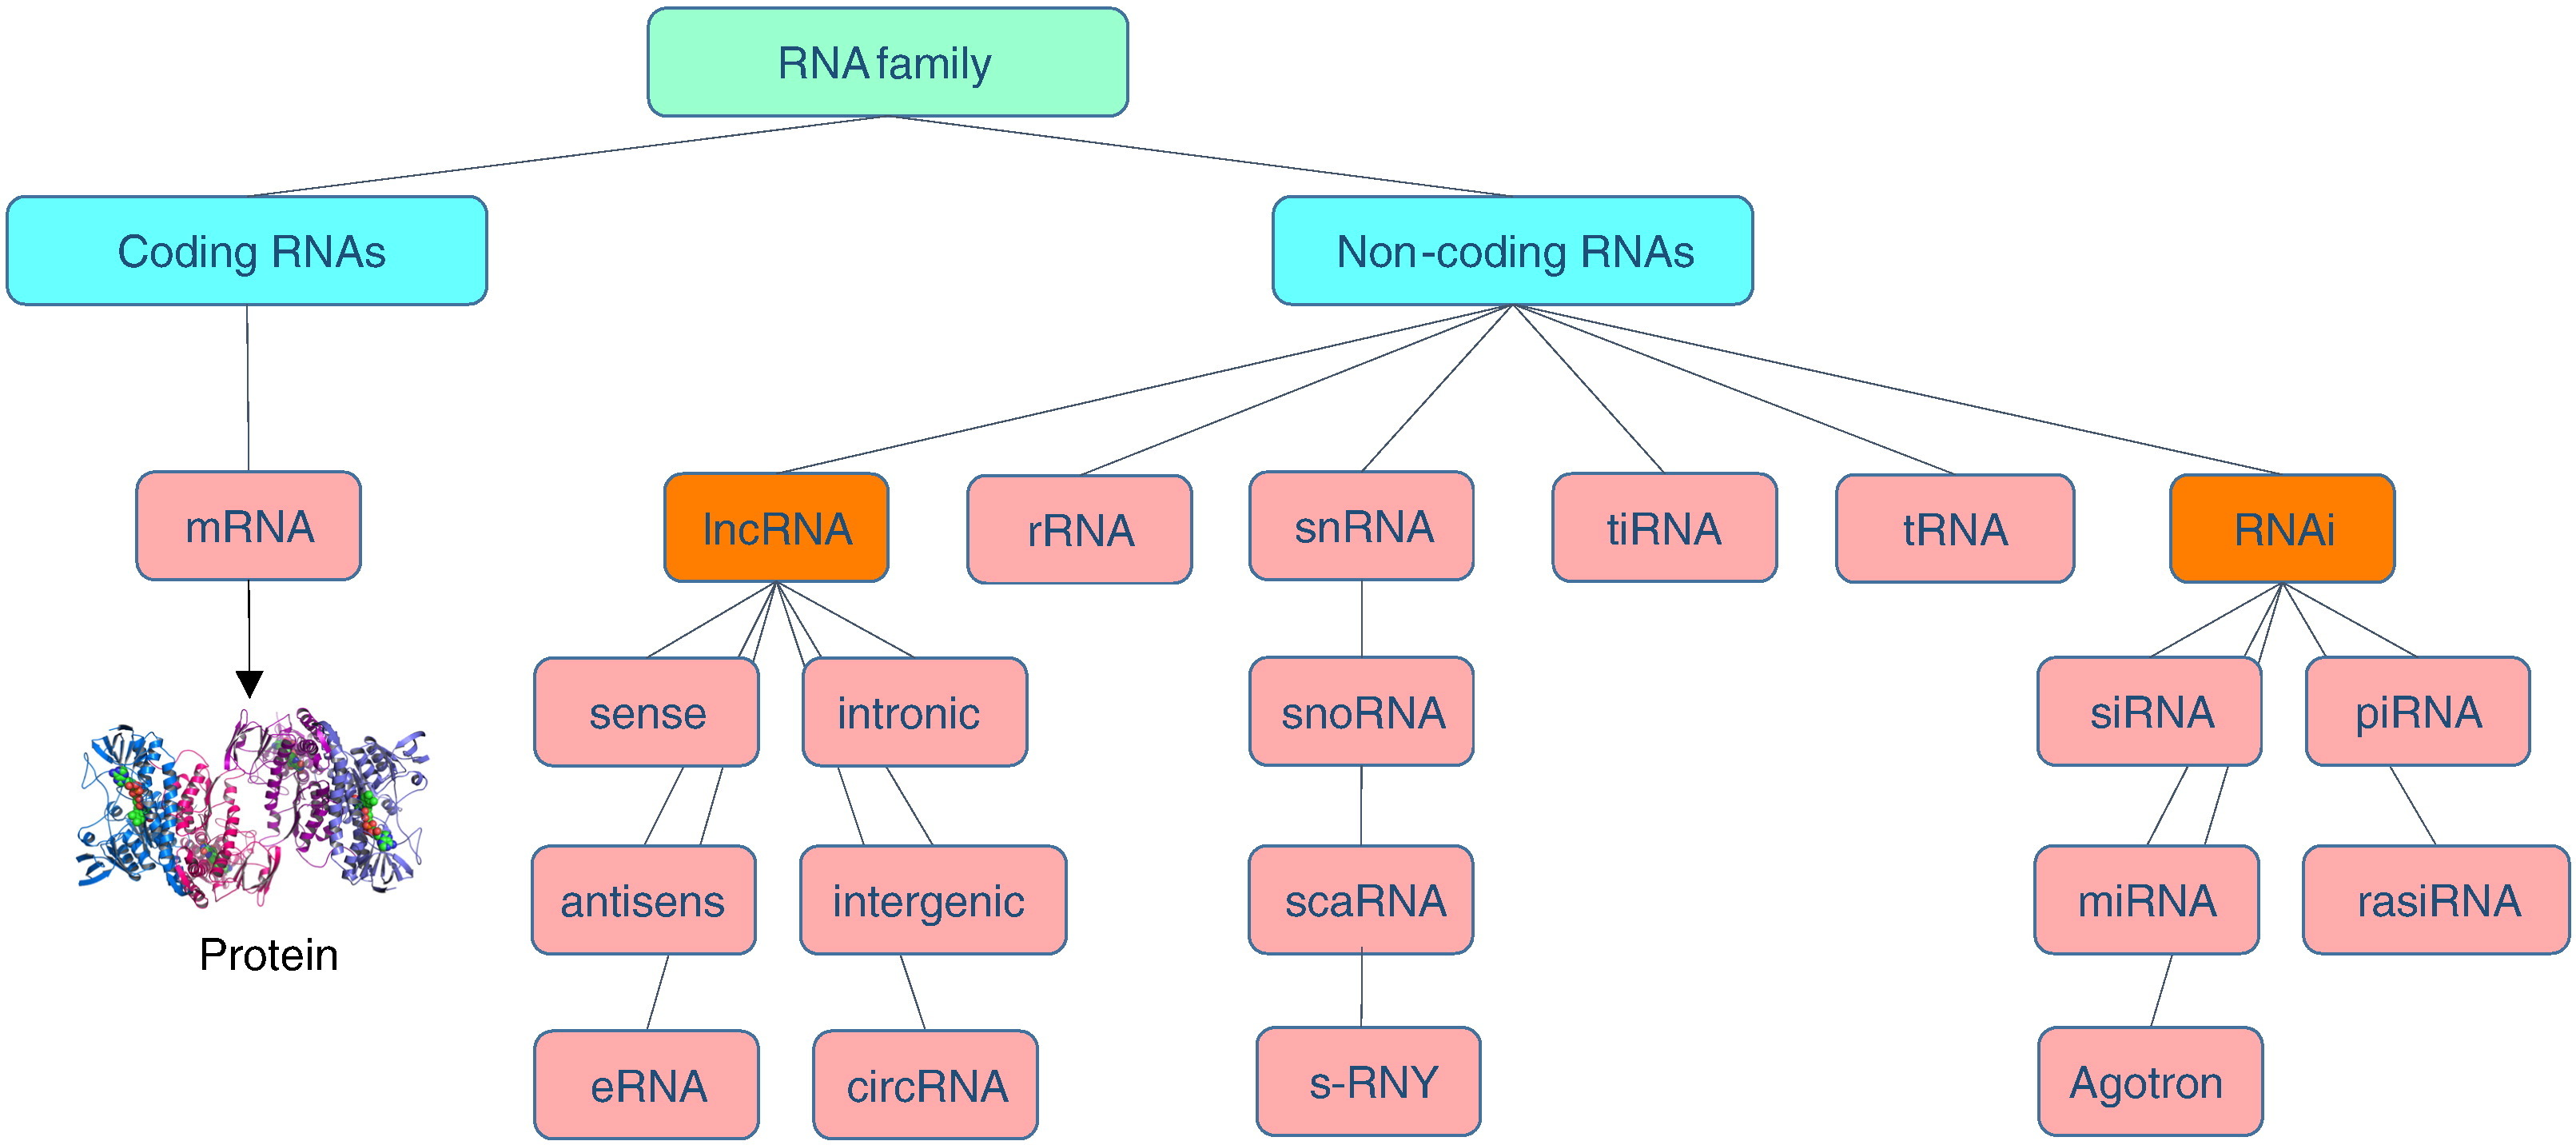
\includegraphics{img/intro/rna_familly_tree.jpg}

%% TRANSITION : parler des erreurs/variabilité biologique ? 

% \subsection{L'étude des perturbation du vivant pour la résolution de conditions cliniques}
\subsection{L'étude des perturbation de l'expression pour la résolution de conditions cliniques}

\section{Les technologies de séquençage de l'expression des gènes}
%% TODO : merge avec 1.1 partie d'avant

%% Nb publi pour le ration de microarray / RNA seq de jeux de données ?


%% historique des techno et qques specificités : https://journals.plos.org/ploscompbiol/article?id=10.1371/journal.pcbi.1005457
\begin{itemize}
\item Avant propos sur le développement des technologies de séquençage avec la quantification d'ARNm par rt-qPCR, le séquençage par gel, etc.
\item Transition vers les technologies de séquençage nouvelle génération
\end{itemize}

%% Un TRES bon site sur les technos de sequencage : http://education.knoweng.org/sequenceng/

\subsection{Microarray}
\begin{itemize}
\item Principe
\item Utilisation avec des exemple
\item Propriétés mathématiques et techniques
\begin{itemize}
    \item Distribution
    "Données continues, il est possible de construire des modèles d’analyse statistique ense basant sur des hypothèses de normalité des données (Smyth, 2004). Ces techniquesd’analyse, adaptées aux données gaussiennes ne peuvent pas être appliquées directementaux données RNA-seq qui sont des données de comptage, discrètes et positives" %% https://tel.archives-ouvertes.fr/tel-01424124/document
    \item Normalisation : Normalization is a process designed to identify and correct
technical biases. 2 types of norm : Between and within normalization (cf. formation marie laure meme si c'est pour le RNA-seq). Pourquoi normalisation log2 : le log pour passer à une échelle symétrique autour de 0, le 2 car c'est + facile à interpréter, chaque fois qu'on augmente le ratio Ti de 1, on double la up regulation  %%(https://www.researchgate.net/post/Why_do_we_usually_use_Log2_when_normalizing_the_expression_of_genes et https://www.nature.com/articles/ng1032z)
    \item Contrôle qualité
    \item Filtration
\end{itemize}
\item Explication du déclin mais avec contraste sur son utilité quand pas besoin de whole transcriptome
\end{itemize}

\subsection{RNA-Seq}
\begin{itemize}
\item Principe
\item Un mot sur le fait qu'on applique pas les mêmes méthodes de normalisation car la nature du signal n'est pas le même : une fluorescence pour le microarray (variable continue), et un comptage dans le cas du RNA-seq (variable discrète).
\item Explication de l'essor du RNA-seq (couts, precision, etc.)
\item Propriétés mathématiques : distribution(binomiale negative) %% Justification binomiale negative "Negative binomial (NB) distribution is the established gold standard, because of its ability to accurately model RNA-seq data with a low number of available replicates [7]." https://doi.org/10.1093/bib/bbx115
\item normalisations : %% cf. formation marie laure, il y a toutes les refs de publi a prendre
%% La raison du l'utilisation des pseudo counts et du log dans le RNA-seqyo : https://www.biorxiv.org/content/biorxiv/early/2020/05/19/2020.05.19.100214.full.pdf
\begin{itemize}
    \item Within sample
    \item Between samples
\end{itemize}
%% À classer entre within/between plus ahut selon ce qui est marqué dans la formation de marie laure : taille de librairie (= profondeur de sequencage), contenu en GC, taille des gènes, composition de la population d'ARN de chaque condition), contrôle qualité, filtration  (https://www.biostars.org/p/349881/)
\end{itemize}


%%%%%%%%%%%%%% LE TRAITEMENT STATISTIQUE DE L'INFORMATION BIOLOGIQUE %%%%%%%%%%%%%%


\section{Le traitement statistique de l'information biologique}
\subsection{L'expression différentielle : les acteurs majeurs}
\begin{itemize}
  \item Méthode de capture des acteurs majeurs
  \item Pas d'étude du système 
% \item Des statistiques descriptives à l'expression différentielle %% Bof, j'ai pas retrouvé de stade "stats explo" 
\end{itemize}

\subsection{La modélisation du vivant : des acteurs au système}
\begin{itemize}
\item De la régulation des gènes à son approximation par des modèles statistiques, en passant par la biologie des systemes qui est trop couteuse pour des organismes complexes %% mal formulé car dans le desordre (le dernier point devrait venir en 2e)
\item Transistion vers la modélisation par encodage de l'information dans des réseaux qui sont en fait des graph et qui sont moins couteux car probabilistes (ils ne sont pas la vérité mais une approximation)
\end{itemize}

\subsection{Les réseaux biologiques : le système vu via la théorie des graphes}
\begin{itemize}
\item Principe : les graphes sont une méthode de plus en plus utilisée dans la représentation du fonctionnement d'organismes puisqu'ils permettent d'avoir une vision à l'échelle du système tout entier.
%% Jolie intro à s'inspire : https://www.nature.com/articles/s41467-019-08746-5
\item Différences / ressemblance entre graphe et reseau ?
\item Les types de réseaux/graphes rencontrés en biologie et plus particulièrement en expression des gènes : small-world
\item Les problèmes de visualisation de grands réseaux %% section layout de ce livre https://sites.fas.harvard.edu/~airoldi/pub/books/BookDraft-CsardiNepuszAiroldi2016.pdf
\end{itemize}


%%%%%%%%%%%%%%%%%% LES RESEAUX DE CO-EXPRESSION %%%%%%%%%%%%%%%%%%


\section{Les réseaux de  co-expression}

%% GROOOOOSSSE PUBLI REVIEW sur la co-expression ET la comparaison de modules, aka co-expr differentielle https://doi.org/10.1109/TCBB.2019.2893170

\subsection{But}
"Gene co-expression networks seek to identify transcrip- tional patterns indicative of functional interactions and regulatory relationships between genes" %%https://genomebiology.biomedcentral.com/articles/10.1186/s13059-019-1700-9 + Barabási A-L, Gulbahce N, Loscalzo J. Network medicine: a network-based approach to human disease. Nat Rev Genet. 2011;12:56–68. + Furlong LI. Human diseases through the lens of network biology. Trends Genet. 2013;29:150–9.

\subsection{Principe}
%% Relire `van Dam, S., Võsa, U., van der Graaf, A., Franke, L. & de Magalhães, J. P. Gene co-expression analysis for functional classification and gene–disease predictions. Brief. Bioinform. bbw139 (2017). doi:10.1093/bib/bbw139`
\begin{itemize}
    \item Réseaux binaires (0 = pas de connexion, 1 = connexion). Pour et contres.
    \item Réseaux pondérés. Pourquoi c'est vers ça qu'on s'est orientés ? Car les connections entre gènes ne sont pas binaires, elles sont plutot multiples et très dépendantes temporellement. Une meme cellule échantillonnée à des temps différents aura un profil plus ou moins différent. On y retrouvera les grandes fonctions clefs mais les aspects plus variables auront peut etre changé. D'où aussi la nécessité d'un bon nombre d'échantillons pour assurer la validité des résultats. Sinon les correlations ne sont pas représentatives.
\end{itemize}
\subsection{Construction}
\begin{itemize}
\item Les différents scores de similarité : Pearson, Spearman, bicor, mutual information
\item La pondération des scores (adjacence et TOM) et la propriété d'invariance d'échelle (scale-free). Reparler de barbarasi et son celebre article (https://science.sciencemag.org/content/325/5939/412/tab-pdf) + Pourquoi elle est parfois encore discutée (https://www.nature.com/articles/s41467-019-08746-5) alors que tout de même pertinente en biologie. 
\end{itemize}
\subsection{Détection de modules}
\begin{itemize}
    \item Notion de communauté
    \item Définition du partitionnement (clustering) et des différentes techniques
\end{itemize}

\subsection{Exploitation des modules de gènes}

\subsubsection{Intégration biologique}
%% AKA knowledge driven
\begin{itemize}
    \item Enrichissement
    \item Test d'association
\end{itemize}

\subsubsection{Association phenotypique}
%% aussi knowledge driven

%%\subsection{Capitalisation sur l'information intrinsèque aux données}

\subsubsection{Étude topologique}
%% AKA data driven

%% Note : à voir si je présente aussi ici la comparaison de module vu que je vais ptet évoquer l'expression differentielle ici pour faire le parallele avec l'analyse transcripto classique. Sinon ça ira dans l'intro du chapitre avec l'article de GWENA.

\begin{itemize}
    \item Degré
    \item Définition de hub gene
    A trier / ordonner entre les différentes définitions, ce qu'elles visent, ce qu'elles appaortent et si possible une comparaison d'entre elles. On distinguera les mesure purement basées sur la theorie des graphs et celles impliquant des mesures statistique de significativité d'un gene comme hub (cf publi sur DHGA)
    \begin{itemize}
        \item Def 1 : Network theory : "A node is defined as hub node, if its connection degree is greater than average connection degree of the network" %% https://www.ncbi.nlm.nih.gov/pmc/articles/PMC5215982/
        \item Def 2 : Network hubs, the core elements in the network, can be defined using a range of different measures. These measures quantify distinct aspects of topological centrality, which can be defined as the capacity of a node to influence or be influenced by other nodes by virtue of its connection topology (Fornito et al., 2016).
    \end{itemize}
\end{itemize}
\subsubsection{Expression différentielle}
Pas sur de foutre ca là... Peut etre plutot en intro de la section complete en guise de "En analyse RNA classique, une méthode data driven est l'expression différentielle, mais en co-expression on a a disposition plus d'information extractable, et ce grace a la theorie des graphes" 

\subsubsection{Comparaison de modules}

Ou co-expression différentielle
%% "However, searching for differences in networks requires great sensitivity to the initial choice of data. For example, the absence of a shared link in mouse and human co-expression networks does not necessarily indicate divergent function. Instead, differences in the mouse and human co-expression networks may indicate differences in the technical platforms or the experimental conditions used to build the networks" http://doi.org/10.1371/journal.pgen.1000776

\subsection{Interprétation des résultats}

\subsubsection{Comparabilité des résultats issus de RNA-seq et de microarray}
\begin{itemize}
    \item Pas les meme hub genes %% "Microarray and RNA-seq-derived networks have different hub genes" https://academic.oup.com/bioinformatics/article/31/13/2123/196230
\end{itemize}


%%%%%%% L'INTÉRÊT DE l'ANALYSE PAR CO-EXPRESSION POUR L'ÉTUDE DU VIEILLISSEMENT %%%%%%%


\section{Le vieillissement, système hautement imbriqué}
%% Idée de début de paragraphe
S'il est une condition biologique où les réseaux de co-expression sont particulièrement bien adpatés, c'est bien le vieillissement. Source multi-factorielle de changements dans l'organisme, il est chez l'humain à l'origine d'une dégradation progressive des fonctions de base du corps.

\subsection{Définition biologique}
\begin{itemize}
    \item Facteurs : raccourcissement des télomères, phénomènes d'inflammation, réduction de la machinerie cellulaire
    \item Manifestation : Ralentissement de la division cellulaire, développement de cellules non-fonctionnelles / nocives (aka tumeurs), malfonctionnement des tissus/organes
\end{itemize}

\subsection{Enjeux}
Un enjeu de santé publique
\begin{itemize}
    \item Susceptibilité aux maladies opportunistes
    \item tdeetAutonomie patient
    \item Médicalisation précoce
\end{itemize}

\subsection{La capture de l'information liée au vieillissement par la transcriptomique}

\begin{itemize}
    \item La dérégulation de la transcription comme phénomène précédemment mentionné
    \item L'insuffisance de la capture de biomarqueurs pour un processus aussi compliqué que le vieillissement. Donc la nécessité d'une étude en réseau
    \item 
    
\end{itemize}
%% https://doi.org/10.1007/978-981-32-9005-1_3


\section*{Phrases utiles à retravailler et intégrer}

\begin{itemize}
\item "Studies have shown that each gene is estimated on average to interact with four to eight other genes1 and to be involved in 10 biological functions" [10.1038/s41598-017-18705-z]
\item "A very clear partition of different biological networks is provided by Christensen et al. [1], who separated these networks into five main categories as follows: [metabolic networks, signal transduction networks,transcriptional regulatory networks, protein-protein networks, functional gene networks]" [10.1093/bfgp/elt003]
%% Bouquin à la coloc de Clément à Sète, pas retrouvé sur le net jusque là 
\item "Le vieillissement est un continuum conduisant une personne en bonne santé à une réduction de sa réserve fonctionnelle, puis de sa capacité fonctionnelle et de sa qualité de vie. CEs différents aspects ne décrivent pas un chemin linéaire ou ordonné." [Patient agé : particularités de la consultation, Gilles Berrut]
\item "It has been reported that nearly one in four studies uses public data to address a biological problem without generating new raw data (Rung and Brazma, 2013)." [10.3389/fpls.2016.00444]
\end{itemize}


%% Points que je veux aborder :
%%  - Definition des reseau arrete / noeud
%%  - Definition des modules par l'effet de modularité
%%  - Ce à quoi ils peuvent servir : raccrochage de fonction a certains genes, detection de pathways, detection de reseaux de regulation



%%    • Weighted aspect [trop general, aura plutot sa place dans la thèse]
%% But because of the multi-functionality aspect of each gene, such GCN using only binary state between genes (1 = correlated, 0 = not correlated) lead to information loss\cite{Langfelder2008}. Therefore, a new class of GCN have been developed: weighted gene co-expression networks. One of the most famous implementation is the R package WGCNA\cite{Langfelder2008}, but one can also mention the recent wTO\cite{Gysi2018} package which consider both positive and negative correlation for GCN building. Instead of a simple pairwise correlation, these packages weight the similarity score by calculating a factor taking into account other properties of the network. In the case of WGCNA, it specifies an adjacency score which raise the similarity to a power, which will increase the strength of strong similarities while keeping low week ones. In the case of wTO, it determine an average accounting for all common neighbors of a node.

%%    • Topological aspect
%%    • Co-expression properties (Scale-free-network entre autres ?)



%% Infos sur la peau : these super interessante => https://dumas.ccsd.cnrs.fr/dumas-01599807/document% \end{itemize}

                          % introduction
% \setcounter{chapter}{2}
% \setcounter{section}{2}
\chapter{Chapitre 1 - GWENA: gene co-expression networks analysis and extended modules characterization in a single Bioconductor package}
\label{chapter:gwena}


\section{Résumé}

% 150 mots max, imposé par FESP
L'analyse de l'expression des gènes par le biais de réseaux de co-expression peut être utilisée pour étudier les relations modulaires entre des gènes remplissant différentes fonctions biologiques. À ce jour, aucun outil ne combine en un pipeline pérenne les analyses usuelles ainsi que la co-expression différentielle et la visualisation de réseau. Nous présentons ici GWENA, un nouveau progiciel R disponible sur Bioconductor qui répond à ce besoin. Pour démontrer ses performances, nous avons appliqué GWENA sur deux ensembles de données de muscle squelettique provenant de patients jeunes et âgés de l'étude GTEx. De façon remarquable, nous avons priorisé plusieurs gènes pour l'étude du vieillissement ainsi que précisé le phénomène connu de perte de connectivité. En effet, parallèlement à cette déconnexion se déroule une reconnexion de divers gènes sur les gènes pivots du réseau, gènes codant pour des mécanismes de compensation.


\section{Abstract}
\subsection{Background}
Network-based analysis of gene expression through co-expression networks can be used to investigate modular relationships occurring between genes performing different biological functions. An extended description of each of the network modules is therefore a critical step to understand the underlying processes contributing to a disease or a phenotype. Biological integration, topology study and conditions comparison (e.g. wild vs mutant) are the main methods to do so, but to date no tool combines them all into a single pipeline.

\subsection{Results}
Here we present GWENA, a new R package that integrates gene co-expression network construction and whole characterization of the detected modules through gene set enrichment, phenotypic association, hub genes detection, topological metric computation, and differential co-expression. To demonstrate its performance, we applied GWENA on two skeletal muscle datasets from young and old patients of GTEx study. Remarkably, we prioritized a gene whose involvement was unknown in the muscle development and growth. Moreover, new insights on the variations in patterns of co-expression were identified. The known phenomena of connectivity loss associated with aging was found coupled to a global reorganization of the relationships leading to expression of known aging related functions.

\subsection{Conclusion}
GWENA is an R package available through Bioconductor (\url{https://bioconductor.org/packages/release/bioc/html/GWENA.html}) that has been developed to perform extended analysis of gene co-expression networks. Thanks to biological and topological information as well as differential co-expression, the package helps to dissect the role of genes relationships in diseases conditions or targeted phenotypes. GWENA goes beyond existing packages that perform co-expression analysis by including new tools to fully characterize modules, such as differential co-expression, additional enrichment databases, and network visualization.

\subsection{Keywords}
co-expression network, differential co-expression, R package, pipeline, aging, skeletal muscle




%%%%%%%%%%%%%%%%%%%%%%%%%%%%%%%%%%%%%%%%%%%%%%%%%%%%%%%%%%%%%%%%%%%%%%%%%%%%%%%%%%%
%%   Background                                                                  %%
%%%%%%%%%%%%%%%%%%%%%%%%%%%%%%%%%%%%%%%%%%%%%%%%%%%%%%%%%%%%%%%%%%%%%%%%%%%%%%%%%%%

\section{Background}


The study of biological functions through discrete genes analysis methods has allowed the elucidation of numerous pathways and the understanding of gene-disease associations \citeA{Barabasi2004}. The full comprehension of the complex interactions taking place in cellular processes requires methods that are able to grasp the connections between the genes involved \citeA{Hartwell1999}. To address this issue, biological networks have been used as a framework to represent and study relationships between genes. In a gene network, a node represents a gene and an edge joining two nodes represents their relationship. Among the measures of relationship, weighted co-expression is one of the most widely used thanks to the popularity of the WGCNA R package \citeA{Langfelder2008} where the relationships are quantified (weight) instead of only a presence/absence information. The use of gene co-expression networks thus led to important discoveries such as the characterization of functional elements in \textit{Arabidopsis} \citeA{Mao2009}, help with prognosis in breast cancer \citeA{Tang2018}, and more generally identification and prioritization of disease candidate genes \citeA{Graaf2017}. 

When constructing gene co-expression networks, existing tools usually follow the same methodology. Using either microarray or RNA-seq gene expression, a co-expression score based on correlation is computed between each pair of genes in the samples. A clustering method is then selected to detect groups of strongly co-expressed genes called modules. The search for meaning in the co-expression relations classically involves the integration of biological information, as well as the study of topology \citeA{Graaf2017}. Biological integration usually involves two methods, namely gene set enrichment and phenotypic association \citeA{Graaf2017, Langfelder2008}. A phenotypic association is based on the correlation between the eigengene (a representative of gene expression profile) of the module and a phenotype measured on the samples. Despite typically having a low yet significant correlation \citeA{Zhang2013}, phenotypic associations are used as a surrogate to study the molecular changes related to a condition. By looking for the genes responsible for the correlation, this method serves as a means of causal genes discovery or a way to find the effect of the condition on the phenotype \citeA{Tseng2013}. As for the gene set enrichment, the most common enrichment test is based on the over-representation analysis (ORA) of a group of genes (in this case modules) compared to a reference of biological annotations such as Gene Ontology (GO) \citeA{Ashburner2000} or Reactome \citeA{Fabregat2016}. This approach, based on the guilt-by-association approach, allows the identification of new gene functions. The consideration of the scale-free topology property of gene co-expression networks also allow the use of graph theory metrics and methods to analyze the networks from a new perspective.
The highly-connected genes also known as hub genes are often relevant for the functionality of the module, either being a regulator \citeA{Pierson2015} or a gene coding for an essential function \citeA{Hahn2005}. Their detection and the investigation of the neighboring gene is therefore an opportunity to understand the mechanisms at work.

Like differential expression analysis, co-expression analysis can be used in a differential way to compare conditions (e.g.:wild vs. mutant). This method aims to isolate dissimilarities \citeA{Chowdhury2019} that would not be found by solely studying the GCN of a condition of interest (e.g. disease, phenotype). Variations in gene co-expression between multiple conditions can translate into appearance/disappearance of modules, changes in gene composition of a module, or rearrangement of genes within a module potentially leading to separation into several other modules \citeA{Graaf2017}. These modifications of patterns reveal insights on the biological alterations in modules of interest and can suggest possible regulatory events linked to the studied condition (e.g. : transcription factors, miRNA). Such concepts were used successfully in recent publications to  detect specific gene modules involved in ovarian or breast cancer \citeA{Gov2017, Bhuva2019} or in recovery from water stress in \textit{Cleistogenes} \citeA{Yan2019}.

To date, multiple tools exist that perform one or few of the functionalities described previously but none combine them all into a single pipeline. Moreover, no available tool includes differential co-expression, exploits the potential of other topological metrics such as connectivity, or enables analysis to be carried out with other R packages or software as easily. In order to meet all these needs, we developed an R package for Gene Whole co-Expression Network Analysis (GWENA) available on Bioconductor (\url{https://bioconductor.org/packages/release/bioc/html/GWENA.html}). Based on a modified version of WGCNA for the network construction and module detection, GWENA is a modular pipeline that provides ORA enrichment on 9 biological sources, phenotypic association, hub genes detection, and differential co-expression between multiple conditions. These come with a set of descriptive visualizations that help the user understand and interpret complex results of gene co-expression network analysis.

In order to demonstrate the capabilities of our tool, we applied it to investigate skeletal muscle aging using publicly available gene expression data from donors spanning different age ranges from the GTEx database (ref). Skeletal muscle aging is indeed a major source of mobility loss in the elderly, resulting in a high fall ratio, depression, and therefore an increased mortality \citeA{Bulut2017}. This decrease in the regenerative capacity of skeletal muscles and their progressive atrophy (sarcopenia) \citeA{Santilli2014} gradually leads to a reduction of the contractile force and thus a loss of autonomy of the individuals \citeA{Janssen2002}. Recent studies have made progress in finding factors associated to evolution of sarcopenia \citeA{Sakuma2017, Bulut2017}, such as body weight \citeA{Jiao2017}, but the understanding of their intricate molecular mechanisms is still lacking.

In this article, we will therefore provide details on the implementation of our new R package GWENA. A presentation of its application will be done with the study of gene co-expression in young muscle, and then in the context of skeletal muscle aging by comparing samples from younger and older donors.  Finally, a qualitative comparison will be made with other existing tools.


%%%%%%%%%%%%%%%%%%%%%%%%%%%%%%%%%%%%%%%%%%%%%%%%%%%%%%%%%%%%%%%%%%%%%%%%%%%%%%%%%%%
%%   Implementation                                                              %%
%%%%%%%%%%%%%%%%%%%%%%%%%%%%%%%%%%%%%%%%%%%%%%%%%%%%%%%%%%%%%%%%%%%%%%%%%%%%%%%%%%%

\begin{figure}[ht]
    \centering
    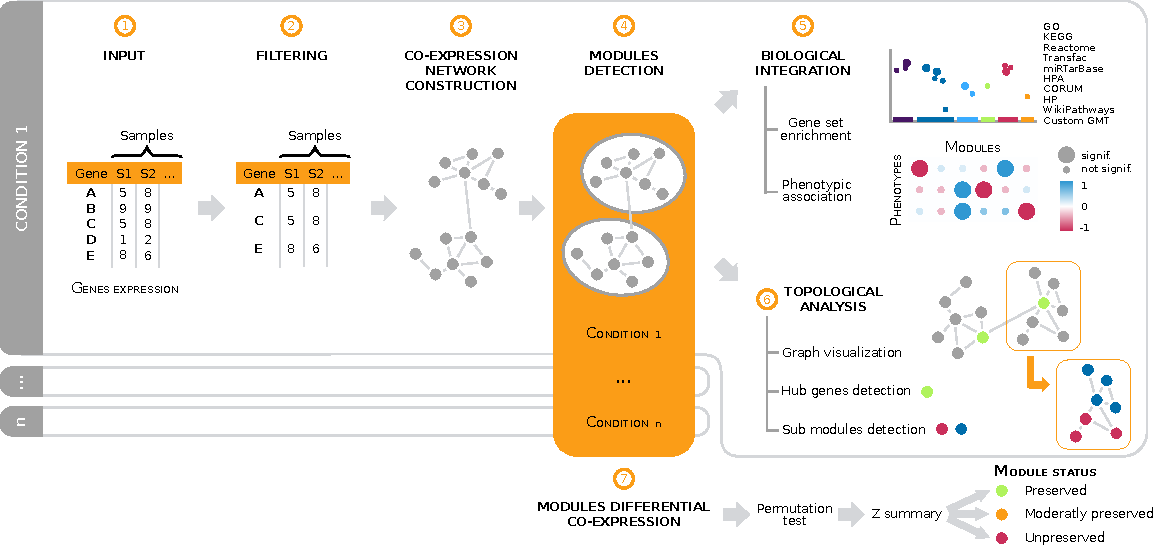
\includegraphics[width=0.95\textwidth]{img/chap1/figure_1.pdf}
    \caption[Detailed steps of analysis performed in GWENA's pipeline]{Detailed steps of analysis performed in GWENA's pipeline, from expression data to characterization of the modules and comparison of conditions. \textcircled{\small{1}} Input : expression matrix pre-normalized and aggregated to gene level if it is a transcript matrix. \textcircled{\small{2}} Filtering : optional genes filtration according to transcriptomic input technology. \textcircled{\small{3}} Co-expression network construction : computation through modified WGCNA function of a correlation matrix on the gene expression matrix, then transformation into an adjacency matrix, and finally into a topological overlap matrix (TOM). \textcircled{\small{4}} Modules detection : genes clusterization over the TOM with another modified WGCNA function. \textcircled{\small{5}} Biological integration : gene set enrichment of each module using g:Profiler services, and phenotypic association if a phenotype matrix is provided to describe the samples. \textcircled{\small{6}} Graph analysis : transformation of the TOM in a graph to compute different topological metrics, detect the hub genes, and detect sub-modules of one module. \textcircled{\small{7}} Modules differential co-expression over N conditions : permutation test using NetRep combined with a Z summary to detect preserved or unpreserved modules.} 
    \label{fig:fig_pipeline_schema}
\end{figure}


\section{Implementation}

Designed as an R Bioconductor package, GWENA is a modular pipeline intended to ease the construction, interpretation and comparison of GCN. It reproduces a classical GCN analysis reinforced by complementary tools (Fig. \ref{fig:fig_pipeline_schema}). 


\subsection{Input}

Both microarray and  RNA-seq normalized expression can be used as input. The choice of normalization method is left to the user as it is highly dependent on the technology used to produce the raw data and the experimental design. Data must be stored in a table with genes as columns and samples as rows, or in a SummarizedExperiment object \citeA{morgan1summarizedexperiment2018}. The minimal number of samples recommended is about 20 samples \citeA{Langfelder2014FAQ} with 100 samples ensuring a more robust networks \citeA{Liesecke2019}.

Transcript-level data (probes or transcript) need to be aggregated to the gene level for the next steps (i.e. probes measurement summarized to their corresponding gene) \citeA{miller2011}. Its execution is left to the user as the transcriptomic technology impacts the aggregation method to choose. However, it is recommended to use the highest mean probes expression for microarray data, and the counts sum for RNA-seq. This can be achieved with the collapsing R function as described by Miller et al. \citeA{miller2011}.


\subsection{Filtering}

Genes are not always informative for modules detection as genes not always vary and their expression can be linked to technical biases. An additional filtering step can thus be applied to avoid noise and speed up the pipeline analysis. This operation must be carried out with caution as it may impact the network construction. Over-filtering may result in loss of informative signal and changing the data distribution could break the scale-free topology \citeA{Parsana2019, Langfelder2014FAQ}. In addition, co-expression network analysis is a method designed to handle larger amount of data than differential expression analyses and can capture more subtle significant gene expression variation \citeA{Hudson2009,Tseng2013}.

Two filters meeting these criteria are available in GWENA:
\begin{enumerate}
    \item Low count filter : removes genes having a lower count than a pre-defined threshold (default is 5). It prevents confusing the true expression of a gene with an expression due to technical background noise. 
    \item Low variation filter : removes genes which expression is too similar across samples. As co-expression modules detection relies on the discrimination of similarity between gene expression profiles across samples, genes that so not vary sufficiently across samples may be randomly clustered in the same (or in different) modules which would not reflect the biological reality.
\end{enumerate}


\subsection{Co-expression network construction}

The well-known R package WGCNA \citeA{Langfelder2008} was modified in order to be integrated it in our modular pipeline : the co-expression network construction step which computes the genes pairwise co-expression score has been isolated in its own R function. The first step of the co-expression score computation is the calculation of a correlation matrix based on the gene expression matrix. The Spearman correlation was added to the automated version of network construction in WGCNA as it ensures a better representation of genes monotonic relationships \citeA{Song2012}.
A power law distribution is then fitted on the correlation matrix and the “correlation matrix is then raised to the estimated power, resulting in an adjacency matrix \citeA{Yip2007}. According to the hierarchical organization of gene co-expression networks \citeA{Ravasz2003}, a topological overlap matrix (TOM) \citeA{Yip2007} is then computed using the adjacency matrix which represents the final gene co-expression score matrix.
Finally, the function return this matrix along with metadata information regarding the computation to ensure a good tracking of the performed operations.


\subsection{Modules detection}

The modules detection part from WGCNA was isolated in a new R function using the previously calculated gene co-expression score matrix as input. A hierarchical clustering is performed on the matrix which is then cut according to the dynamic cut tree method \citeA{Langfelder2008_cutree} in order to define the modules and the genes they contain. The first component of the principal component analysis of each module is used as a representative of their respective gene expression profile and is called an eigengene. In addition to its summarizing function, the eigengene is used to merge the highly-correlated modules. The gene co-expression profile of each module is visible using a dedicated function, with the eigengene highlighted. The function finally returns a detailed object with the detected modules as lists of genes identifiers, the dendrogram of the clustering, and the modules before merge. 


\subsection{Biological integration}

Biological integration consists of two different analyses, namely gene set enrichment and phenotypic association. 

The gene set enrichment (or functional enrichment) analysis is performed using g:Profiler \citeA{Raudvere2019} through their gprofiler2 R package. Their enrichment function covers 9 biological functional databases: Gene Ontology (GO) \citeA{Ashburner2000}, Kyoto Encyclopedia of Genes and Genomes (KEGG) \citeA{Kanehisa2019}, Reactome \citeA{Fabregat2016}, Transfac \citeA{Matys2006}, miRTarBase \citeA{Chou2018}, Human Protein Atlas (HPA) \citeA{Uhlen2015}, CORUM \citeA{Ruepp2008}, Human Phenotype ontology (HP) \citeA{Kohler2019}, WikiPathways \citeA{Slenter2018}. Realizing a custom enrichment file through a Gene Matrix Transposed (GMT) format in gprofiler2 requires the use of additional functions. Also, gprofiler2 does not provide a merging function between the output of classical and custom enrichment to return all the enrichments in a single output. GWENA therefore provides a wrapper of these functions to have an all-in-one function.

The phenotypic association uses the eigengene returned in the output of the module detection function to perform a correlation test on a matrix of given phenotypes. If a phenotype is qualitative instead of quantitative, the variable encoding the phenotype is transformed into a binary variable (also known as dummy variable). 


\subsection{Graph analysis}

To analyze the topology of the graph and allow its visualization, GWENA imports the igraph \citeA{Gabor2009} R package. A wrapping function including integrity checks use the gene co-expression score matrix to build a graph object on which all igraph topological metrics can be computed (e.g. degree, connectivity, strength). 
Among the multiple metrics computable on a network, hub genes remain the most studied structure. As they can be defined according to different methods, the three most popular ones were implemented: highest connectivity \citeA{Azuaje2014}, highest degree \citeA{Tseng2013}, and Kleinberg's score \citeA{Kleinberg1999a}. 
GWENA visualization function simplifies the native plotting function of igraph and adapts it to GCN to assist in their interpretation (e.g. the native implementation of an edge filter parameter, as these are complete graphs). The layout selection was also favored towards scale-free topology compatible layouts as they are a main property of GCN.
Sub-modules within previously detected modules can provide valuable information about the distribution and communication between biological functions within a module. GWENA allows their detection by performing a partitioning around medoids (PAM) clustering method \citeA{Kaufmann1987, Schubert2019} with an automatic estimation of the number of cluster through a silhouette coefficient. These sub-modules can also be passed to the graph plot function to display them and see their organization.


\subsection{Modules differential co-expression}

Analysis of module preservation or non-preservation can be performed between different conditions such as treatments or phenotype. To isolate modules whose topology changes between conditions, GWENA first performs a permutation test using the NetRep R package \citeA{Ritchie2016}. Seven topological metrics are computed on each module in each condition. A permutation is then applied to the selected control condition where each node label of the modules is randomly reassigned without replacement to another and the seven metrics are then recomputed on it. Using these permutations as a null distribution \citeA{phipson2010}, modules are considered preserved if all seven topological metrics are significant for the alternative hypothesis (one or two-sided) with the chosen alpha error.

As the unpreservation of a module cannot be assumed from the non significant modules, a second step of preservation evaluation is carried out using a Z summary score \citeA{Langfelder2011, Li2015}. The final score returned by GWENA is the combination of these two steps (Additional file 1: Figure S1).



%%%%%%%%%%%%%%%%%%%%%%%%%%%%%%%%%%%%%%%%%%%%%%%%%%%%%%%%%%%%%%%%%%%%%%%%%%%%%%%%%%%
%%   Results and discussion                                                      %%
%%%%%%%%%%%%%%%%%%%%%%%%%%%%%%%%%%%%%%%%%%%%%%%%%%%%%%%%%%%%%%%%%%%%%%%%%%%%%%%%%%%

\section{Results and discussion}

To present GWENA's use and its capability to isolate genes groups or co-expression patterns of interest in a single condition or multiple conditions, we analyzed RNA-seq skeletal muscle data from GTEx (v8)\citeA{GTEx2015} (Additional file 1: Table S1). This data set contains 19,312 genes from 803 samples representing ages ranging from 20 to 70 years old. Low read counts and the low variation genes were discarded using the filtering function of GWENA to decrease the noise, resulting in 18870 genes.

As GTEx data is known to be subject to multiple confounding factors (batch effect, experimental bias, read contamination, etc.) \citeA{Nieuwenhuis2020a,Somekh2019a,Parsana2019}, a partial PC-correction\citeA{Parsana2019} was applied to correct the data (Additional file 1: Figure S2 and S3). To investigate the aging process two subsets representing contrasting age classes were selected from the corrected data set: 73 samples between 20 and 30 years old (referred as young in this report), and 292 samples between 60 and 70 years old (referred as old in this report). Both datasets were analyzed using GWENA's pipeline with default parameters, except for the correlation method parameter which was selected to be "spearman" instead of the default "pearson" as it is less prone to outliers. 

\begin{figure}[p]
    \centering
    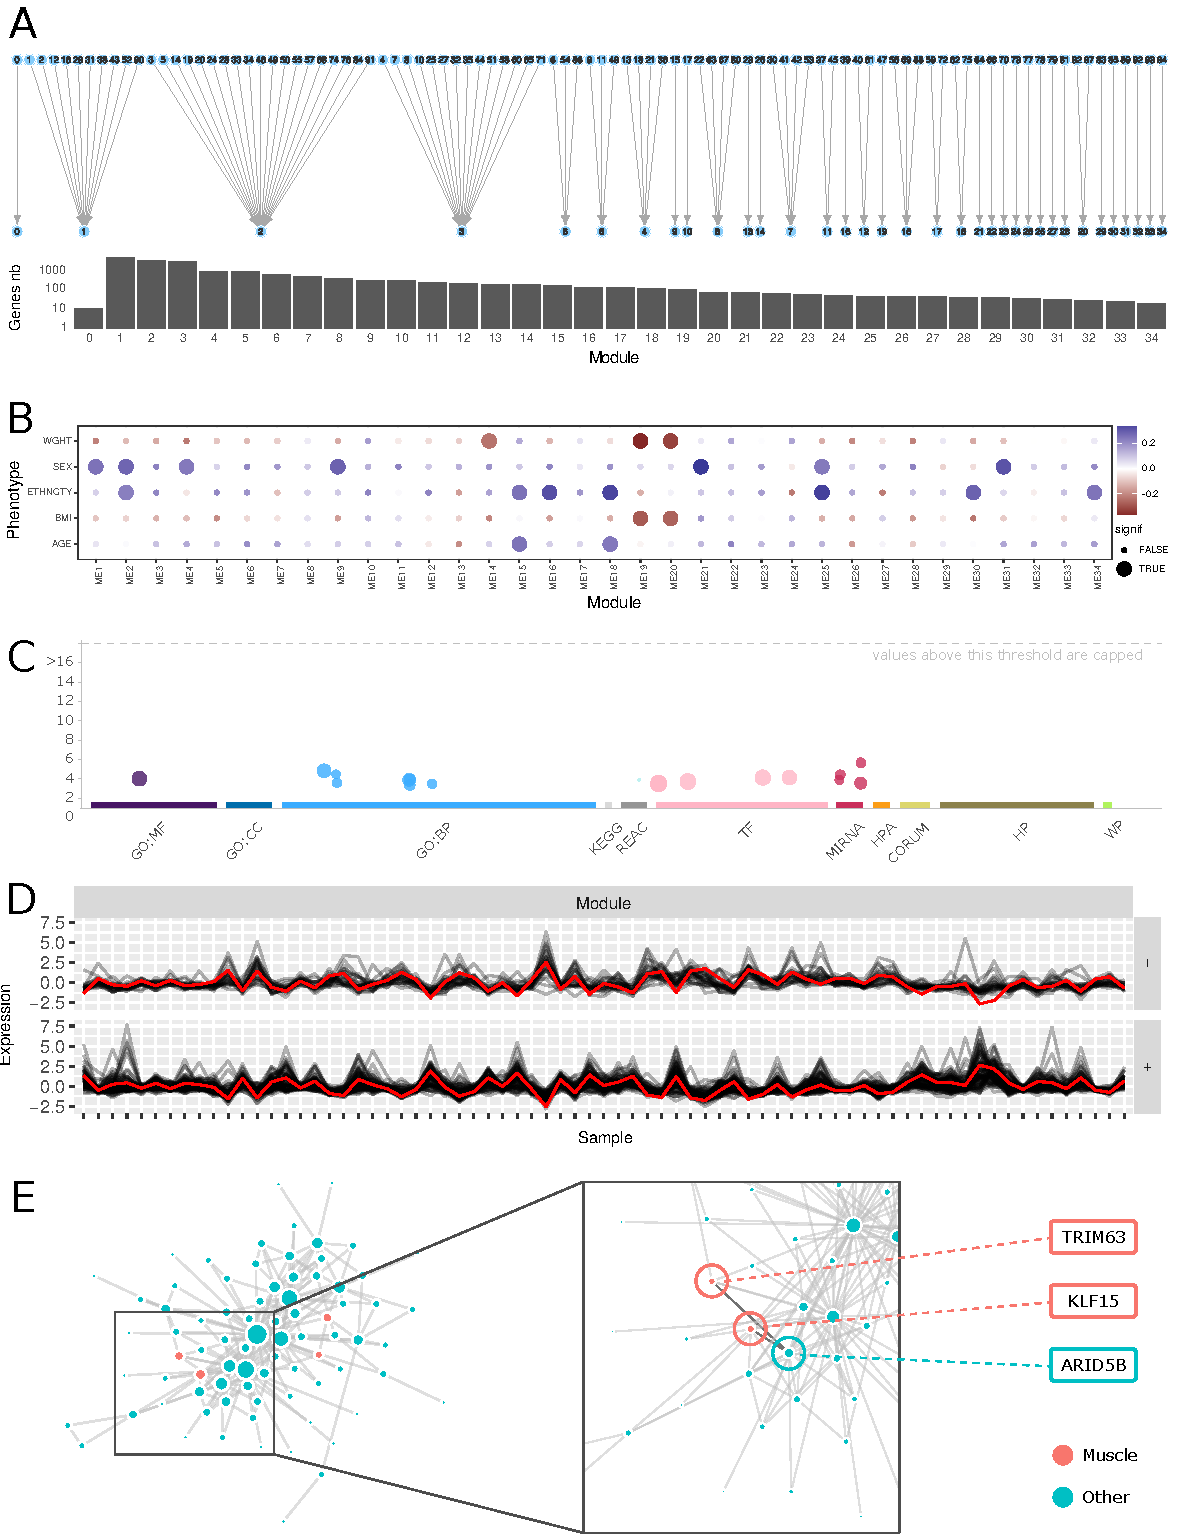
\includegraphics[width=0.90\textwidth]{img/chap1/figure_2.pdf}
    \caption[Available visualizations in GWENA along the pipeline applied to the aging study on the whole age range]{Available visualizations in GWENA along the pipeline applied to the aging study on the whole age range. A : modules merge as a bipartite graph from plot\_modules\_merge function and the genes distribution inside each of them (log scale). B : phenotypic association between the 35 modules and age, sex, BMI, ethnicity, weight. C : Manhattan-like enrichment plot (interactive in GWENA) of module 10 on GO, KEGG, Reactome, Transfac, miRTarBase, Human Protein Atlas, CORUM, Human Phenotype ontology, WikiPathways. D: module 19's network visualization as a graph with muscle enrichment genes colored in red and others in blue. The zoom focus on ENSG00000158022 / ENSG00000107372 / ENSG00000265972 and related hub genes. E : expression profile of module 19 split depending on the correlation sign to the eigengene.}
    \label{fig:fig_resume_visu}
\end{figure}


\subsection{Single condition modules analysis}

To illustrate the process of analyzing a single condition with GWENA, we initially focused on studying the muscle gene co-expression computed in the young sub-population. The 95 modules detected on the co-expression score matrix with GWENA were merged according to their similarity indices, which resulted in a total of 35 modules (Fig \ref{fig:fig_resume_visu}a). Each module was then tested for its association with a selected set of phenotypes related to muscle aging (i.e. age, sex, ethnicity, body weight and BMI) to isolate modules of interest. As shown in Fig. \ref{fig:fig_resume_visu}b, 15 of these modules were significantly associated with at least one of the phenotypes.

These modules were provided to GWENA enrichment analysis (p value \textless 0.05 with g:SCS multiple testing correction) to identify their biological functions and assess their potential involvement in muscle function (Table \ref{table:mod_young_bio_integration_summary}). All modules were at least enriched in one term and 8 obtained enrichment terms related to muscle activity or metabolism (Table \ref{table:mod_young_bio_integration_summary}). Modules 19, 21 and 25 were the top 3 enriched for terms related to muscle function. However, modules 21 and 25 terms were mostly coming from Human Protein Atlas and were also related to a wide range of additional tissues such as the pancreas, the cervix, the bladder, the stomach, or the skin and were thus deemed less specific for muscle aging than module 19. 

Briefly, the remaining module 19 presented 77\% of genes positively correlated to its eigengene (therefore 23 negatively, Fig. \ref{fig:fig_resume_visu}d), and the muscle enriched terms involved muscle adaptation and negative regulation of hypertrophy (Table \ref{table:mod19_enrichments}, Fig. \ref{fig:fig_resume_visu}c). The detection of hub genes by GWENA returned 12 hub genes, some of which are known as transcription factors. Among them, ARID5B (ENSG00000150347) is a transcription factor strongly co-expressed with KLF15 (ENSG00000163884) and TRIM63 (ENSG00000158022) (Fig. \ref{fig:fig_resume_visu}e). These two genes are present in the GO term GO:0014888 (striated muscle adaptation) to which ARID5B is not associated. The function of ARID5B is well known in adipocytes and hepatocytes but is still rarely studied in skeletal muscle metabolism. However, the knockout of this gene in mice has shown structural defects in the sarcomere structure \citeA{Murray2018}.

\begin{table}[H]
\centering
% \resizebox{\columnwidth}{!}{
\begin{tabular}{lllll}
\textbf{module} & \textbf{\# genes} & \textbf{\# pheno. asso.} & \textbf{\# enrichment} & \textbf{\% muscle enrich.} \\ \hline
0               & 11                & NA                       & NA                     & NA                         \\
1               & 5335              & 1                        & 3288                   & 0.6                        \\
2               & 3661              & 2                        & 1098                   & 0.4                        \\
3               & 3355              & 0                        & 1620                   & 0.3                        \\
4               & 1001              & 1                        & 1883                   & 1.0                        \\
5               & 987               & 0                        & 1626                   & 0.0                        \\
6               & 699               & 0                        & 457                    & 0.6                        \\
7               & 546               & 0                        & 428                    & 1.1                        \\
8               & 409               & 0                        & 561                    & 0.7                        \\
9               & 310               & 1                        & 729                    & 0.3                        \\
10              & 308               & 0                        & 58                     & 5.2                        \\
11              & 261               & 0                        & 857                    & 0.0                        \\
12              & 214               & 0                        & 847                    & 15.0                       \\
13              & 207               & 0                        & 452                    & 1.4                        \\
14              & 197               & 1                        & 767                    & 0.5                        \\
15              & 175               & 2                        & 233                    & 0.0                        \\
16              & 137               & 1                        & 6                      & 0.0                        \\
17              & 136               & 0                        & 1                      & 0.0                        \\
18              & 129               & 2                        & 20                     & 0.0                        \\
19              & 108               & 2                        & 18                     & 3.7                        \\
20              & 77                & 2                        & 52                     & 0.0                        \\
21              & 72                & 1                        & 233                    & 2.8                        \\
22              & 63                & 0                        & 24                     & 0.0                        \\
23              & 57                & 0                        & 10                     & 0.0                        \\
24              & 55                & 0                        & 8                      & 0.0                        \\
25              & 47                & 2                        & 82                     & 8.5                        \\
26              & 47                & 0                        & 32                     & 0.0                        \\
27              & 46                & 0                        & 12                     & 0.0                        \\
28              & 43                & 0                        & 147                    & 4.7                        \\
29              & 40                & 0                        & 17                     & 0.0                        \\
30              & 35                & 1                        & 2                      & 0.0                        \\
31              & 31                & 1                        & 12                     & 0.0                        \\
32              & 27                & 0                        & 1                      & 0.0                        \\
33              & 24                & 0                        & 23                     & 0.0                        \\
34              & 20                & 1                        & 3                      & 0.0                       
\end{tabular}
% }
\caption[Summary of detected modules and related biological integration]{Summary of detected modules and related biological integration. The number (\#) of genes is indicated for each module (module 0 being a false module containing the unassigned genes. The number of phenotypic associations with the variables of interest (weight, sex, ethnicity, bmi, age) are counted for each one. The number of enrichments corresponds to the count of significant terms on each cumulative biological database. The ratio (\%) of enriched terms associated with muscle is then established as the number of terms containing one or more elements of the following corpus: "muscle", "sarco*", "*", "muscul*", "actin*", "myosin*" (where * denotes a completion by any other character string)
}
\label{table:mod_young_bio_integration_summary}
\end{table}



 Coupled with the results of GWENA, this may corroborate the involvement of ARID5B in the adaptation of striated muscle in response to a stimulus. Moreover, it has recently been shown that ARID5B knockout in mice was associated with increased glucose metabolism via an increased translocation of SLC2A4 (ENSG00000181856) \citeA{Okazaki2020}. Since SLC2A4 is a gene that is also regulated by KLF15 \citeA{Gray2002, Fan2018}, this supports the idea that ARID5B has implications in skeletal muscle function and more precisely in glucose metabolism. GWENA thus allowed the identification of a gene that may give new insight in the muscle development and growth which needs to be confirmed by further experiments.

\begin{table}[H]
\centering
% \resizebox{\columnwidth}{!}{
\begin{tabular}{lll}
\textbf{source} & \textbf{term name}                                                                                    & \textbf{p val.} \\ \hline
GO:BP           & response to hormone                                                                                   & 0.0015          \\
GO:BP           & \begin{tabular}[c]{@{}l@{}}negative regulation of muscle \\ hypertrophy\end{tabular}                  & 0.0033          \\
GO:BP           & muscle adaptation                                                                                     & 0.0118          \\
GO:BP           & response to peptide hormone                                                                           & 0.0129          \\
GO:BP           & striated muscle adaptation                                                                            & 0.0255          \\
GO:BP           & \begin{tabular}[c]{@{}l@{}}platelet-derived growth factor \\ receptor signaling pathway\end{tabular}  & 0.0328          \\
GO:BP           & regulation of muscle adaptation                                                                       & 0.0434          \\
GO:MF           & enzyme binding                                                                                        & 0.0097          \\
MIRNA           & hsa-miR-6882-5p                                                                                       & 0.0002          \\
MIRNA           & hsa-miR-197-5p                                                                                        & 0.0039          \\
MIRNA           & hsa-miR-152-5p                                                                                        & 0.0125          \\
MIRNA           & hsa-miR-6878-5p                                                                                       & 0.0282          \\
REAC            & \begin{tabular}[c]{@{}l@{}}Regulation of FOXO transcriptional \\ activity by acetylation\end{tabular} & 0.0126          \\
TF              & \begin{tabular}[c]{@{}l@{}}Factor: Zbtb37; motif: \\ NYACCGCRNTCACCGCR; match class: 1\end{tabular}   & 0.0073          \\
TF              & \begin{tabular}[c]{@{}l@{}}Factor: RNF96; motif: \\ BCCCGCRGCC; match class: 1\end{tabular}           & 0.0074          \\
TF              & \begin{tabular}[c]{@{}l@{}}Factor: ETF; motif: \\ GVGGMGG; match class: 1\end{tabular}                & 0.0193          \\
TF              & \begin{tabular}[c]{@{}l@{}}Factor: AP-2; motif: \\ SNNNCCNCAGGCN\end{tabular}                         & 0.0306          \\
TF              & \begin{tabular}[c]{@{}l@{}}Factor: AP-2; motif: \\ SNNNCCNCAGGCN; match class: 0\end{tabular}         & 0.0306         
\end{tabular}
% }
\caption[Module 19 young enriched terms table]{Module 19 young enriched terms table. Multiple enrichment are linked to muscle development and growth}
\label{table:mod19_enrichments}
\end{table}


\subsection{Multiple conditions modules comparison and analysis}

Differential expression analysis allowed the detection of genes involved in aging in the last years (GenAge \citeA{Tacutu2018}, Digital Ageing Atlas \citeA{Craig2015}). Such discriminant analysis is limited in helping to understand aging as this phenomenon is composed of concomitant mechanisms \citeA{Zierer2015}. Understanding the relationships between the genes is therefore crucial to determine the altered functions and the changes involved. Differential GCN between conditions overcomes this problem by detecting the subtle pattern modifications. 
Using our previously defined young (20 to 30 years old) and old (50 to 60 years old) skeletal muscle modules, we ran GWENA's GCN differential co-expression functionality to compare the modules between these age ranges. The GCN of each module detected in the young sub-population were taken as a reference and tested against the ones detected in the old sub-population.

\begin{table}[H]
\centering
% \resizebox{\columnwidth}{!}{
\begin{tabular}{lll}
\textbf{Comparison status} & \textbf{\# modules} & \textbf{Modules id}                                                                                           \\ \hline
preserved                  & 11                  & \begin{tabular}[c]{@{}l@{}}1, 2, 3, 4, 6, 8, 9, 11,\\ 12, 14, 19\end{tabular}                                 \\
moderately preserved       & 17                  & \begin{tabular}[c]{@{}l@{}}7, 10, 13, 17, 18, 20,\\ 21, 22, 23, 24, 25, 27,\\ 28, 30, 31, 33, 34\end{tabular} \\
unpreserved                & 2                   & 16, 32                                                                                                        \\
inconclusive               & 4                   & 5, 15, 26, 29                                                                                                
\end{tabular}
% }
\caption{Modules comparison between young and old age range and their comparison status }
\label{table:comparison_young}
\end{table}


From the 35 modules detected in the previously described single condition analysis of young muscle data, GWENA's differential GCN of young versus old age range returned 2 modules that were unpreserved, 17 modules that were moderately preserved, 11 modules that were preserved, and 4 that were inconclusive (Table \ref{table:comparison_young}, Additional file 1: Figure S1). Unpreserved and moderately preserved modules are the most promising for identifying groups of genes differently expressed with age. Few and heterogeneous significant enrichment terms were associated to unpreserved modules while several moderately preserved modules had enrichment terms known to be linked to aging \citeA{Kuehne2017, Lopez-Otin2013, DeMagalhaes2009, Zierer2015} such as transcription regulation (module 21), cellular stress (modules 20 and 27), immune response (modules 7 and 28), cell proliferation (module 13). 


\begin{figure}[!ht]
    \centering
    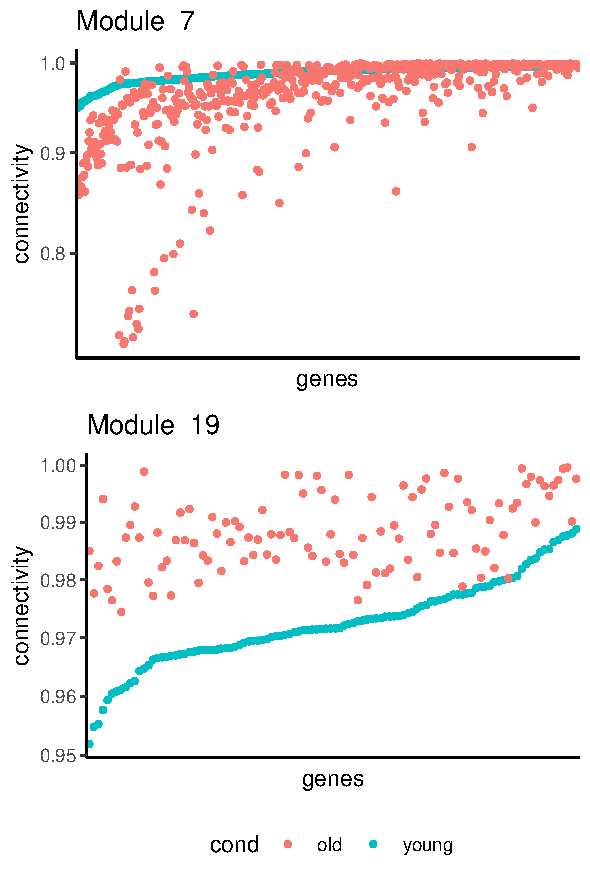
\includegraphics{img/chap1/figure_3.pdf}
    % 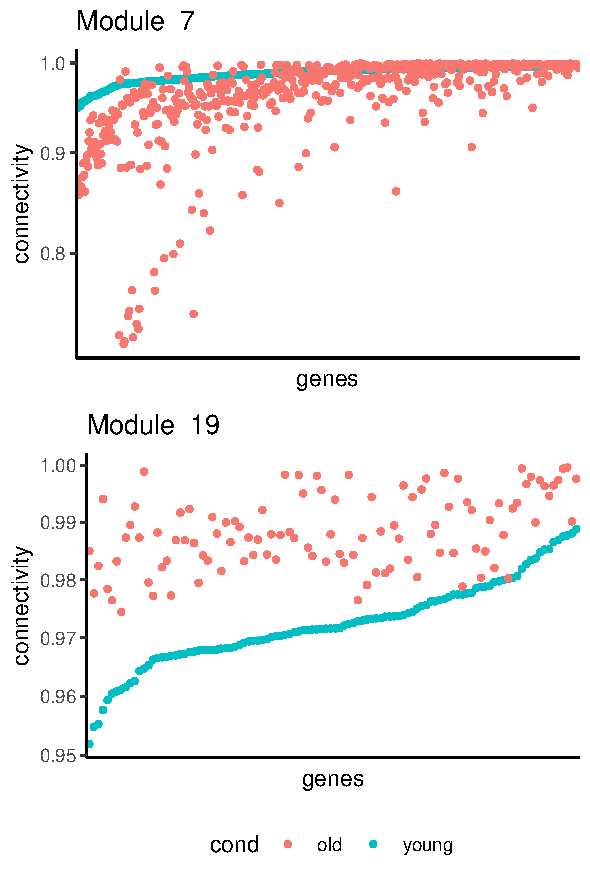
\includegraphics[width=0.95\columnwidth]{img/chap1/figure_3.pdf}
    \caption[Modules 7 and 19 genes (nodes) connectivity distribution between young and old age ranges]{Modules 7 and 19 genes (nodes) connectivity distribution between young and old age ranges. Young age range is used as reference for sorting genes by increasing connectivity. A comparison over all modules can be found in Additional file 1: Figure S4}.
    \label{fig:fig_connectivity_drop}
\end{figure}


In addition to this biological information, the topological comparison of these modules allows to grasp the nature of the variations in the relationships between genes (nodes in the network) and their co-expression score (edge weight in the network). Connectivity, as defined by J. Dong and S. Horwath \citeA{Dong2007}, is a common topological metric computed in GCN as it is representative of the network robustness and is known to be linked to network deregulation \citeA{Anglani2014, Bormann2016}. Over all modules, the connectivity of the genes in module 7 was noticeably dropping between young and old age range (Fig. \ref{fig:fig_connectivity_drop}, Additional file 1: Figure S4). 
Using a co-expression score filter of 0.95, this loss of connectivity materialized in the network through a disconnection (edge loss) of peripheral genes (genes with low degree) such as in sub-module 4 between the young and old age range (Fig. \ref{fig:fig_graph_diff_cluster}a, b). Several other genes of the module 7 from the young age range also showed an increased connectivity when observed in the old age range, which therefore reflects a reconnection (edge gain) to other genes. These results confirm the observations from previous studies of a connectivity loss in the network of modules linked to aging \citeA{Southworth2009, Bormann2016}. Overall, they support an alteration of the transcription regulation.

\begin{figure}[!ht]
    \centering
    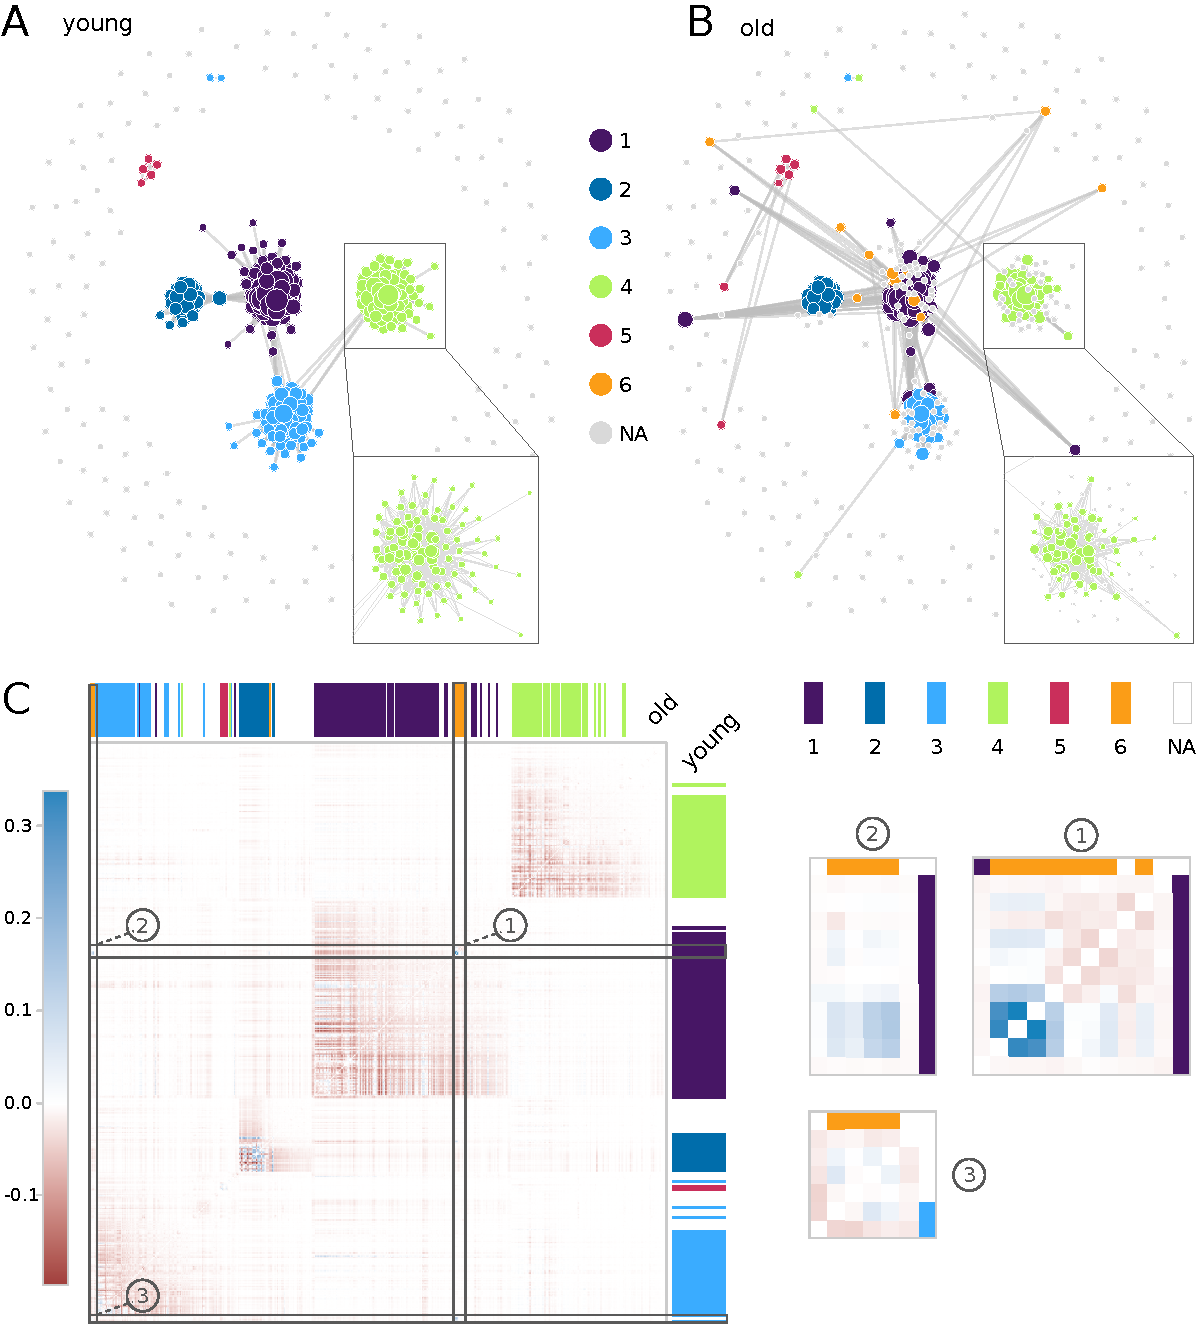
\includegraphics[width=0.95\textwidth]{img/chap1/figure_4.pdf}
    \caption[Module 7 network comparison between young and old]{Module 7 network comparison between young and old. A: module 7 GCN graph plotted with GWENA (0.95 co-expression score filter) for young age range with sub-clusters detected. B: same as A but for the old age range. A zoom is made on sub-module 4 to show the peripheral genes disconnection. The new sub-module 6 is visible in purple in the old graph. C: difference network heatmap (old - young) ordered according to young age range network dendrogram. Sub-modules from old age range are visible on the top of the heatmap in columns, and sub-modules from young age range on the right in rows. Three zooms are made on the heatmap on the areas corresponding to sub-module 6 genes. Zoom \textcircled{\small{1}} contains the genes reconnecting in the old age range.}
    \label{fig:fig_graph_diff_cluster}
\end{figure}

GWENA sub-module detection method on the module 7 revealed an impact of this reorganization of the gene connections by detecting 5 optimal sub-modules for the young age range, and 6 optimal sub-modules for the old age range. The gene composition of the sub-modules was highly similar between the condition (at least 81\% common genes). Most of the differences in the gene composition are due to the disconnection of peripheral genes as previously spotted, and a small portion of the differences are due to the reconnection of genes or their attribution to another sub-module (Fig. \ref{fig:fig_graph_diff_cluster}a, b). This rewiring of the network is in line with known compensatory processes occurring during aging \citeA{Lopez-Otin2013}. By triggering molecular processes involved in limiting or repairing cellular stress damage, these adaptive modifications aim to restore a homeostatic state.

To support this information, the new sub-module (sub-module 6 in Fig. \ref{fig:fig_graph_diff_cluster}b) appearing in the old age range was investigated further. Its creation is at the expense of the sub-module 1 of the young age range and of the 13 genes composing it, 8 of the genes are from the sub-module 1, 3 are reconnecting genes, and 2 are from sub-modules 2 and 3. A gene set enrichment analysis with GWENA of this sub-module 6 revealed significant enrichment in functions related to wound healing, coagulation, vessel diameter, platelet degranulation, and plasminogen activation (Additional file 1: Table S2). This is coherent with known morphological alterations of the vascular system in the aged skeletal muscle \citeA{ElAssar2013, Gopinath2008}, and the global immune/inflammatory response increased in aging \citeA{DeMagalhaes2009}. Also, 51 enrichments from young sub-module 1 were not found significant in any of the sub-modules in the old age range. These enrichments involve antibacterial humoral response and negative regulation of endopeptidase activity. These terms are known to be associated with satellite cells (muscle stem cells responsible for muscle regeneration) regulators released by the vasculature in higher quantity in young skeletal muscle \citeA{Gopinath2008}. 

To complement these analyses, we investigated the variations of co-expression scores leading to the appearance of sub-module 6 in the old age range. Using the network co-expression matrix $\delta$ returned by GWENA for each condition, a co-expression difference matrix (Fig. \ref{fig:fig_graph_diff_cluster}c) was computed such as $\delta_{old} - \delta_{young}$. In this matrix, gene pairs with a negative score indicates a decrease in the co-expression over aging while a positive score indicates an increase in the co-expression. Among the variations, 3 genes showed a significant increase in co-expression between them but also towards other genes of sub-module 6. The pattern visible in Fig. \ref{fig:fig_graph_diff_cluster}c \textcircled{\small{1}} and \textcircled{\small{2}} suggest that these genes may be driving the co-expression changes occurring in this sub-module. These genes are FGG (ENSG00000171557), FGA (ENSG00000171560), and FGB (ENSG00000171564), the three fibrinogen chain coding genes involved in the polymerization of a fibrin matrix. This finding is consistent with previous studies about the increasing fibrinogen content in the elderly skeletal muscle leading to persistent fibrin deposition preventing myofiber repair \citeA{Mann2011, Gligorijevic2018}. They also support the hypothesis of an inflammatory response triggered by a fibrin accumulation. All these results allowed by GWENA's capacity to study the topology and the biological context easily tend to support the idea of not only a global loss in connectivity in aging but also of a gene co-expression reorganization. Our tools also highlighted the biological translation of this reorganization as a potential compensatory response from antibacterial humoral response and endopeptidase activity towards coagulation and wound response.


\subsection{GWENA's contribution and comparison with existing tools}

\begin{table*}[ht]
\resizebox{\textwidth}{!}{
\begin{tabular}{@{}llllll@{}}
\multicolumn{2}{l}{\textbf{Functionalities}}                                                                                      & \textbf{GWENA} & \textbf{WGCNA} & \textbf{CEMiTool} & \textbf{wTO} \\ \midrule
\multirow{5}{*}{\begin{tabular}[c]{@{}l@{}}Gene set \\ enrichment\end{tabular}} & - Gene ontology                                 & yes            & yes            & no               & no           \\
                                                                                & - Pathways (KEGG/Reactome)                      & yes            & no             & no                & no           \\
                                                                                & - Regulation actors (TRANSFAC/miRTarBase)       & yes            & no             & no                & no           \\
                                                                                & - Protein databases (Human Protein Atlas/CORUM) & yes            & no             & no                & no           \\
                                                                                & - Custom GMT import                             & yes            & no             & yes               & no           \\
\multicolumn{2}{l}{Native network visualization}                                                                                  & yes            & no             & no\note{tabfunc}{vizCEMi}               & yes          \\
\multicolumn{2}{l}{Phenotype association}                                                                                         & yes            & yes            & yes               & no           \\
\multicolumn{2}{l}{Hub gene detection}                                                                                            & yes            & yes\note{tabfunc}{hubWGCNA}           & yes\note{tabfunc}{hubCEMi}              & no           \\
\multicolumn{2}{l}{Igraph compatibility for extended topology metrics calculation}                                                & yes            & no             & no                & no           \\
\multicolumn{2}{l}{Sub-module detections inside module \& graph coloration accordingly}                                                                & yes            & no             & no                & no            \\
\multicolumn{2}{l}{Modules differential co-expression}                                                                         & yes            & yes\note{tabfunc}{compWGCNA}           & no                & no\note{tabfunc}{compwTO}          
\end{tabular}
}
\caption[Key features of GWENA compared to similar tools such as WGCNA, CEMiTool and wTO]{Key features of GWENA compared to similar tools such as WGCNA, CEMiTool and wTO. As some differences remain under the same labels, details are provided about their content. \ref{note:tabfunc:vizCEMi}) CEMiTool allows network visualization only if a protein-protein interaction network file is provided, \ref{note:tabfunc:hubWGCNA}) WGCNA only provides a single hub gene selection by module, \ref{note:tabfunc:hubCEMi}) CEMiTool persistently provides the top 10 hub genes independently of the module size or connectivity, \ref{note:tabfunc:compWGCNA}) WGCNA's differential co-expression does not correct for multiple testing, \ref{note:tabfunc:compwTO}) wTO have no differential co-expression method available but provides a consensus network method.
}
\label{table:functionnalities_benchmark}
\end{table*}


Weighted GCN can be computed from existing tools such as WGCNA \citeA{Langfelder2008}, wTO \citeA{Gysi2018}, CEMiTool \citeA{Russo2018}. As both GWENA and CEMiTool use elements from WGCNA, they share notable functionalities. They use similar network construction and modules detection functions from WGCNA but offer their own filter on the datasets. GWENA has been enhanced with additional checks on the network construction (such as aberrant power check) compared to WGCNA and CEMiTool. On its side, wTO used a different version of a topological score to construct the network as they don't perform a power law conversion on the correlation matrix and don't use the same definition of topological transformation. Therefore, the main differences between WGCNA, wTO, CEMiTool and GWENA lie in the added functionalities for module analysis. 

Regarding biological integration, wTO provides neither phenotypic association nor gene set enrichment. The other three tools allow phenotypic association but differ on gene set enrichment analysis. While CEMiTool only allows enrichment on imported GMTs, WGCNA and GWENA allow enrichment on gene ontology. GWENA is the only one allowing enrichment on other databases of pathways, regulatory agents, and proteins (in addition to imported GMTs).

Additional topological analysis functions are also available in several of these tools. The most common, hub gene detection, is present in WGCNA, CEMiTool, and GWENA in different forms. CEMitool and WGCNA offer respectively as hub gene the top 10 most connected genes and genes with a top kME score (membership module based on eigengene). However, methods based on a fixed number of hub genes tend to bias the information since the number of hub genes can vary according to the number of genes present in the module. GWENA therefore proposes several methods (highest connectivity, superior degree, Kleinberg's score) based on a selection of genes with a hub score above a threshold. Another addition specific to GWENA is the ability to re-detect sub-modules into a defined module in order to further investigate the co-expression reconnection organization, and then identify the relations between enrichments associated to each sub-modules by visualizing them on the graph plot.

GWENA includes a differential co-expression analysis in the analysis pipeline as opposed to packages dedicated solely to it (DiffCoEx \citeA{Tesson2010}, CoDiNA \citeA{Gysi2020}, CoXpress \citeA{Watson2006}) or packages like wTO or CEMiTool that do not contain this analysis. The method in GWENA differs from the one present in WGCNA in that it includes a permutation test to prevent the problem of multi-testing. With the addition of the Z-summary score to detect unpreserved modules, GWENA is therefore the only pipeline including a differential co-expression analysis with high confidence in modules found unpreserved. The Table \ref{table:functionnalities_benchmark} finally provide a head-to-head comparison for all functionalities made available by GWENA.

CEMiTool and wTO are built as stand-alone tools with little or no eased interfacing with other tools. WGCNA is similar to them except for exporting networks to Cytoscape \citeA{Hu2014} or VisANT \citeA{PaulShannon2003}. Conversely, GWENA has been developed according to a modular architecture in order to facilitate the realization with an external tool of one of the stages of the analysis pipeline defined in Fig. \ref{fig:fig_pipeline_schema}. GWENA will thus be more easily adaptable to follow future developments in co-expression network analysis methodology.

GWENA, as other GCN analysis tool has limitations. A first one common to all GCN construction method is that the quality of input data (e.g. filtration and/or proper normalization) will inevitably bias the results, especially if it breaks the scale-free property. A second limitation is the design of the permutation test that prevents reporting a significant unpreservation. The non-rejection of the null hypothesis of unpreservation can only state a lack of evidence of preservation. Therefore, unpreserved modules are determined among these modules lacking evidence (the non-significant modules) by the calculation of Z summary which only provide a tendency in the unpreservation \citeA{Langfelder2011}. The present application of GWENA to skeletal muscle aging also presents its own limitation. All analyses were performed on skeletal muscle sample and results were commented regarding this context. However, to be sure of the specificity of the findings, an additional differential co-expression of the modules should be performed on samples from other tissues from subjects with similar age range. As single-cell technologies are becoming common, the differential co-expression could also be used to target the cell-to-cell specific aging variation inside a tissue. Finally, as co-expression networks were unsigned and aging is a complex phenomenon involving actors beyond gene expression, causal effect of any finding need to be experimentally verified. 




%%%%%%%%%%%%%%%%%%%%%%%%%%%%%%%%%%%%%%%%%%%%%%%%%%%%%%%%%%%%%%%%%%%%%%%%%%%%%%%%%%%
%%   Conclusion                                                                  %%
%%%%%%%%%%%%%%%%%%%%%%%%%%%%%%%%%%%%%%%%%%%%%%%%%%%%%%%%%%%%%%%%%%%%%%%%%%%%%%%%%%%

\section{Conclusion}

In this paper, we introduced GWENA, an R package on Bioconductor to construct and analyze GCN in a single pipeline through a whole range of tools from biological integration, topological analysis, and differential co-expression. The package reduces complexity of the GCN analysis through simple input and output functions combined to a set of visualizations to explore the results. The separation of each step of the analysis in one function also allows quick and easy replacement if users wish to use another method for this block.

GWENA demonstrated its performances on both single and multiple condition analysis through an exploration of variations of skeletal muscle function and processes in aging. The single condition analysis showed it is possible to find new genes potentially involved in an existing GO annotation using hub genes, network neighboring genes and gene sets enrichments. The differential co-expression analysis between young and old samples isolated modules specifically linked to aging and detected the rearrangement in connectivity related to aging. Additional analysis supported the observed genes co-expression reorganization beyond simple connectivity loss. This resulted in a reinforcement of previous supposition on inflammatory response to fibrin increases in skeletal muscle aging.	



\bibliographystyleA{unsrt}
\bibliographyA{chap1-biblio}
% \bibliographystyleA{plain-fr}
% \bibliographyA{bibliographie}                         % chapitre 1
\chapter{Chapitre 2 - Analyse trans-tissus par réseau de co-expression de gènes pour la détection de fonctions physiologiques communes et spécifiques au vieillissement}
\label{chapter:multidim}

\section{Introduction}

La variation de la distribution de la co-expression des gènes associée au vieillissement est une propriété qu'on a pu observer dans le muscle auparavant \citeB{Lemoine2021Dec}. Grâce à elle, on a pu isoler des gènes dont la fonction physiologique \citeB{Keeling2019Nov} est confirmée comme liée au vieillissement du muscle. On peut alors considérer l'étude de la topologie des réseaux de co-expression de gènes comme une méthode efficace pour la détection de gènes biomarqueurs du vieillissement dans un tissu. 

Cependant, le vieillissement est un phénomène qui ne se limite pas au muscle dans un organisme et touche bien d'autres tissus en parallèle. Dans chacun d'eux, le transcriptome est un témoin des modifications liées à l'avancée dans l'âge \citeB{DeMagalhaes2010}. Via son analyse par expression différentielle et d'autres méthodes d'analyse de gènes discrètes \citeB{Barabasi2004}, nombre de gènes (biomarqueurs) associés à l'âge ont pu être détectés dans les différents tissus du corps humain. Si pour certains de ces gènes on a déjà étudié leur relation avec des fonctions physiologiques, ce n'est pas le cas de la majorité. Suite à ces études fines de certains gènes, il est également rare bien qu'intéressant de connaître comment leur relation évolue plus globalement, au-delà des fonctions physiologiques considérées.
% Ce manque d'information sur les relations est dû au coût et à la longueur des méthodes pour obtenir les relations entre deux ou quelques gènes. En effet, elles requièrent le plus souvent des expérimentations basées sur des inactivations ou sur-activation d'un ou plusieurs gènes (respectivement \textit{knockout} et \textit{knockin} en anglais). 
Pour pouvoir investiguer chaque relation et impact de chaque gène, la méthode courante implique le plus souvent de réaliser des expérimentations d'inactivation ou sur-activation d'un ou plusieurs gènes (respectivement \textit{knockout} et \textit{knockin} en anglais). Le coût important de ces manipulations, tant en temps qu'en argent limite alors une réalisation en masse pour caractériser en masse les relations entre deux ou quelques gènes. 
L'information apportée par de tels liens permettrait pourtant d'aider à déterminer le type de modification observé \citeB{Lopez-Otin2013}. Ainsi on pourrait estimer si l'activation ou répression du gène observé est le fruit d'une réponse à l'activation d'un autre gène voir mécanisme \citeB{Bechtel2013} complet, ou plutôt l'origine d'un mécanisme avec ou sans autres gènes impliqués.

Ces questions ont d'autant plus d'intérêt que des études précédentes tendent à démontrer l'existence de bases communes au vieillissement tant en termes de fonctions physiologiques que de mécanismes \citeB{DeMagalhaes2009a}. On relève ainsi des signatures d'expression de gènes communes à plusieurs tissus dans leur état "âgé". Parmi les fonctions physiologiques détectées comme sur-exprimées par l'expression différentielle, on retrouve notamment des composantes de la réponse immunitaire ou inflammatoire et de la dégradation lysosomale. À l'opposé, dans les fonctions détectées comme sous-exprimées, on retrouve des fonctions associées à l'encodage de protéines mitochondriales ainsi que des gènes responsables de la production de différents types de collagène. En complément, bien que ne concernant pas tous les tissus du corps, d'autres signatures sont communes à des sous groupes de tissus partageant des propriétés tant moléculaires que cellules. On retrouve par exemple une accumulation de marques de réparation de l'ADN chez les tissus se renouvelant rapidement \citeB{Armanios2012}, un épuisement des capacités de régénération chez les tissus disposant d'une cache de cellules souches \citeB{Ratajczak2017}, des dommages à l'ADN plus présents chez les tissus soumis à des stress mécaniques \citeB{Kubben2017}.

L'analyse de co-expression de gènes a démontré sa capacité à aider à la détermination de nouveaux liens, de nouvelles voies de signalisation dans un tissu \citeB{Hughes2000}. 
Fort de ces réalisations, on s'est interrogé quant à la capacité de la co-expression différentielle à détecter des acteurs du vieillissement non pas simplement entre deux tranches d'âges, mais ceux-ci transversalement à de multiples tissus humains. 
Les différences observées pourraient permettre, contrairement à l'analyse mono-tissu, d'explorer spécifiquement les phénomènes du vieillissement communs ou bien uniques aux différents tissus. 
Par cette démarche, on va ainsi montrer dans chacun de ces cas la détection de nouveaux gènes candidats et à prouver l'intérêt de la co-expression différentielle pour y parvenir.
Une première phase de traitement des données issues de différents tissus a tout d'abord permis de s'assurer de leur comparabilité entre tissus. 
% On a ensuite effectué une exploration générale des modules de gènes obtenus via une revue des fonctions physiologiques et des gènes pivots détectés dans chacun. 
Après une détection des modules de co-expression, on a isolé les modules variant avec l'âge à l'aide d'une analyse de co-expression différentielle pour chaque tissu. Tous ont été recoupés entre eux pour sélectionner les gènes variants en commun. Deux branches ont alors été explorées avec un exemple détaillé dans chacune : les intersections de tissus présentant des phénomènes communs du vieillissement, et les intersections de tissus présentant des phénomènes de vieillissement spécifiques. 
% Nos résultats montrent que dans chacune de ces branches, on est parvenu à identifier des gènes à la fonction encore peu comprise ou bien non associée aux tissus considérés.
Nos résultats montrent que dans chacune de ces branches, on est parvenu à une compréhension plus fine de la fonction de gènes jusqu'à là peu étudiés dans le vieillissement et même plus globalement pour certains.




\section{Matériel et méthodes}

\subsection{Contextualisation des données}

Les données de GTEx étant l'un des rares jeux de données à contenir autant de tissus sains différents et en grand nombre, on les a à nouveau utilisées. Pour approfondir les informations données lors du chapitre \ref{chapter:gwena}, ces données sont le regroupement d'échantillons prélevés sur 54 tissus (+1 tissu qui est en fait un assemblage de lignées cellulaires dérivées de patients atteints de leucémie myéloïde aiguë\citeB{Way2020}) et 980 donneurs dans sa dernière version, la v8. Cette variété de tissus vise à être le plus représentatif possible des différents tissus chez l'humain au vu du coût de prélèvement et d'analyse de chaque échantillon. Les biopsies sont effectuées sur des donneurs décédés avec leur accord préalable, l'accord d'un proche ou l'accord du représentant légal. Elles sont réalisées sur 4 centres de collecte, puis analysées sur place ou transférées selon le tissu avec réfrigération durant le transport. Ces échantillons sont évalués sur plusieurs critères pour jauger leur admissibilité et échantillon non conforme est exclu de la cohorte. On retrouve : 
\begin{itemize}
    \item des critères cliniques : absence de contamination au VIH, absence de chimiothérapie dans les 2 ans, absence de transfusion sanguine dans les 48 h, etc.
    \item des critères anatomopathologiques : absence de tissu cancéreux, absence de pathologie tissulaire, etc.
    \item des critères analytiques : quantité de tissu prélevé suffisante, quantité d'ARN extrait final supérieur à 500 ng d'ARN total, nombre d'intégrité d'ARN ou RIN supérieur à 5.7) \citeB{Carithers2015}. 
\end{itemize}
% des critères cliniques (absence de contamination au VIH, absence de chimiothérapie dans les 2 ans, absence de transfusion sanguine dans les 48 h, etc.), des critères anatomopathologiques (absence de tissu cancéreux, absence de pathologie tissulaire, etc.) et des critères analytiques (quantité de tissu prélevé suffisante, quantité d'ARN extrait final supérieur à 500 ng d'ARN total, nombre d'intégrité d'ARN ou RIN supérieur à 5.7) \citeB{Carithers2015}. Tout échantillon non conforme est exclu de la cohorte.

Sur la majorité des échantillons ont été effectué des séquençages de génome (\textit{Whole Genome Sequencing}, WGS), des séquençages d'exome complet (\textit{Whole Exome Sequencing}, WES), des séquençages de transcriptome (aussi appelé séquençage d'ARN, RNA-Seq), ainsi que des images de coupes histologiques colorées. Des données reformatées sont également mises à disposition telle que les locus de caractères quantitatifs (\textit{quantitative trait loci}, QTL) et l'expression de gène qui est ce que l'on va utiliser ici. Ces données sont disponibles sur le site du consortium GTEx (\url{https://gtexportal.org}) accompagnées d'information sur le phénotype des échantillons. En raison du fort potentiel d'identification des donneurs, le phénotype donné publiquement est partiel, et le phénotype complet est disponible sur demande auprès de dbGaP après soumission d'un dossier de projet à renouveler chaque année (Annexe \ref{annexe:dbgap}).


Par ailleurs, tous les donneurs n'ont pas pu être prélevés pour l'ensemble des 54 tissus et ce sont en moyenne 23,4 tissus qui ont été prélevés sur la version 8 de l'étude GTEx. Certains tissus ont été priorisés lors des biopsies : tissu adipeux (sous-cutané), artère tibiale, cœur (ventricule gauche), poumon, muscle (squelettique), nerf tibial, peau (exposée au soleil), thyroïde, sang complet. Parmi les différents tissus biopsiés, il est à noter que certains sont issus d'un même organe et on a ainsi 31 organes biopsiés pour 54 tissus biopsiés en tout.

% \todo[inline]{Un Sankey diagramme des tissus avec col 1 = SMTS, col 2 = SMTSD, col 3 = tranche d'age à 10 ans}


\subsection{Sélection des tissus}

\begin{figure}[h]
    \centering
    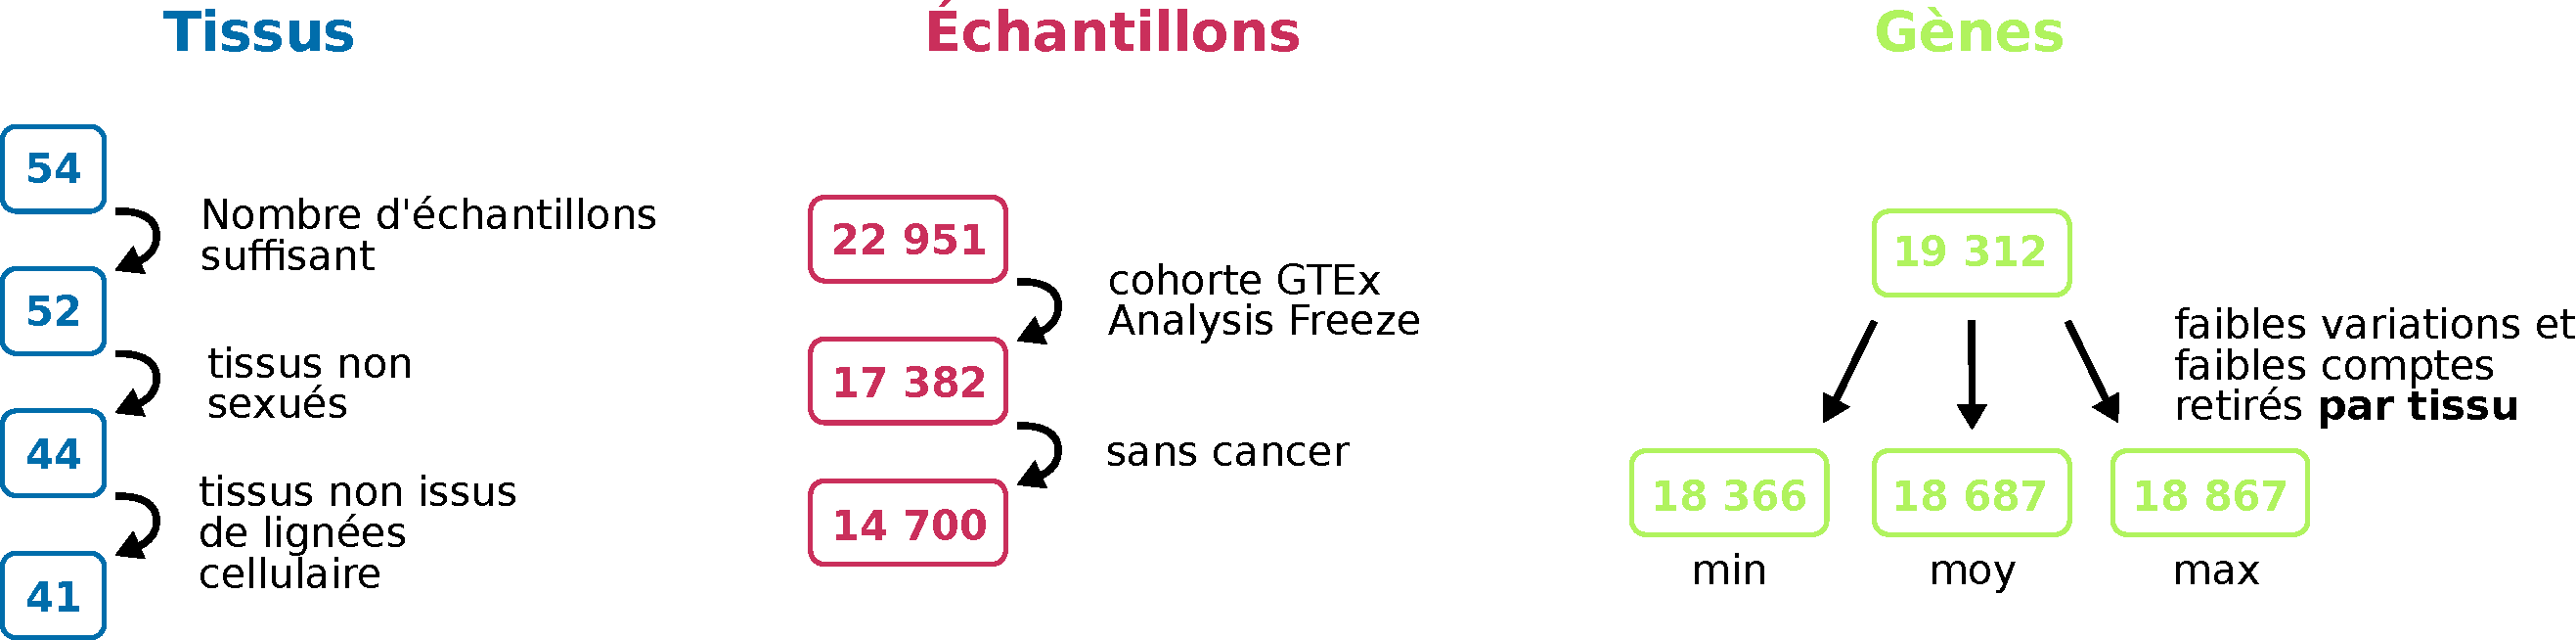
\includegraphics[width=1\textwidth]{img/chap2/chap2_filtre_donnees.pdf}
    % \includesvg[scale=.5]{img/chap2/chap2_filtre_donnees.svg}
    \caption{Ensemble des filtres appliqués sur les différentes données et impact sur les données utilisées pour la construction ultérieure des réseaux de co-expression.}
    \label{figure:data_filters}
    % \caption{Nombre d'échantillons disponibles par tissu et par tranche d'âge de 10 ans dans les données de GTEx.}
\end{figure}


Le vieillissement est un phénomène dont les altérations moléculaires sont linéaires avec le temps, dont les dommages cellulaires sont super-linéaires \citeB{Todhunter2018}, et où la mortalité associée augmente de façon exponentielle passée 20 ans \citeB{Finch2016}. Afin de faciliter la détection de ces altérations grâce à l'analyse de co-expression différentielle, on s'est donc dans un premier temps concentré sur une sélection de tranches d'âges très contrastées. Les échantillons sélectionnés sont issus de donneurs entre 20 et 30 ans pour la tranche qu'on nommera "\textbf{jeune}", et entre 60 et 70 ans pour la tranche qu'on nommera "\textbf{âgée}". Les données de GTEx ne comportent toutefois pas un nombre d'échantillons similaire pour chacune de ces tranches du fait de la mortalité plus importante chez les personnes âgées que les personnes jeunes. Ce déséquilibre est principalement dû aux causes de décès pour chaque tranche d'âge avec des décès par traumatisme chez les jeunes plutôt que par maladie chronique ou maladie liée à l'âge chez les âgés. Un premier filtre de notre pré-traitement restreint donc la sélection des tissus à ceux comportant au minimum 50 échantillons dans chacune des tranches d'âge, ce qui n'est pas le cas de la Vessie (20) et le Rein - Médulla (3). Ce nombre d'échantillons permet d'assurer un bon compromis entre des réseaux de co-expression de gènes robustes, donc non sensibles à des valeurs aberrantes, et la perte de plus de tissus à étudier dans cette analyse multidimensionnelle qu'on souhaite effectuer \citeB{Liesecke2019}.

Tous les tissus restant n'étaient pas nécessairement adaptés à l'étude globale du vieillissement chez l'humain. Ainsi on a retiré tous les tissus liés à un seul sexe : Trompes de Fallope, Col de l'utérus, Utérus, Vagin, Sein, Ovaire, Prostate, Testicule. À ce retrait s'ajoute celui des échantillons de lignées cellulaires (dérivées ou non de tissus eux conservés) car non représentatifs du vieillissement biologique : Cellules - Lymphocytes transformés par EBV, Cellules - Fibroblastes cultivés, Cellules - Lignée cellulaire de leucémie (CML). 


\begin{figure}[ht]
    \centering
    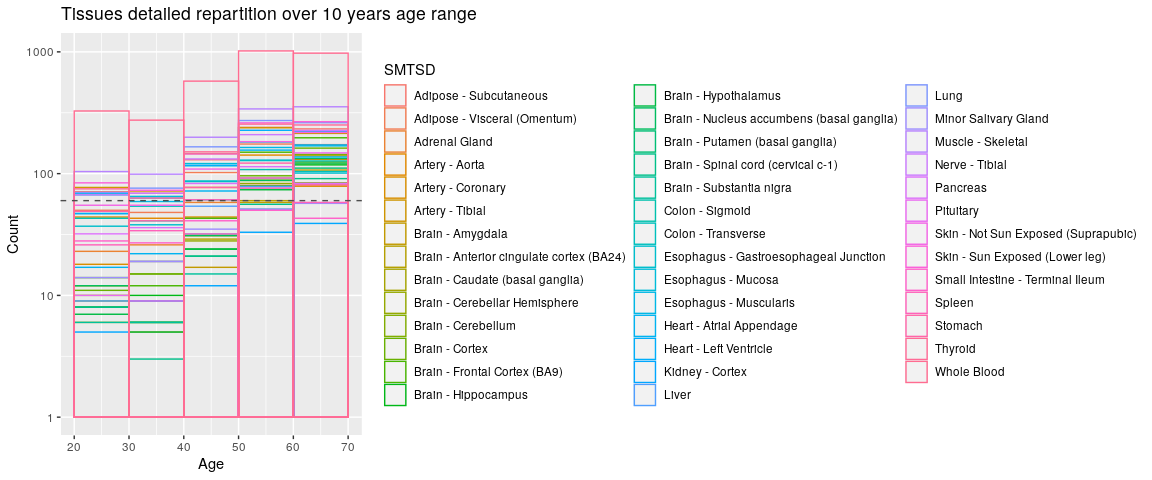
\includegraphics[width=1\textwidth]{img/chap2/chap2_sample_count_by_tissu.png}
    \caption{Nombre d'échantillons disponibles par tissu et par tranche d'âge de 10 ans dans les données de GTEx.}
    \label{figure:sample_count_by_tissu}
\end{figure}


\subsection{Filtre des échantillons}

\begin{figure}[hb]
    \centering
    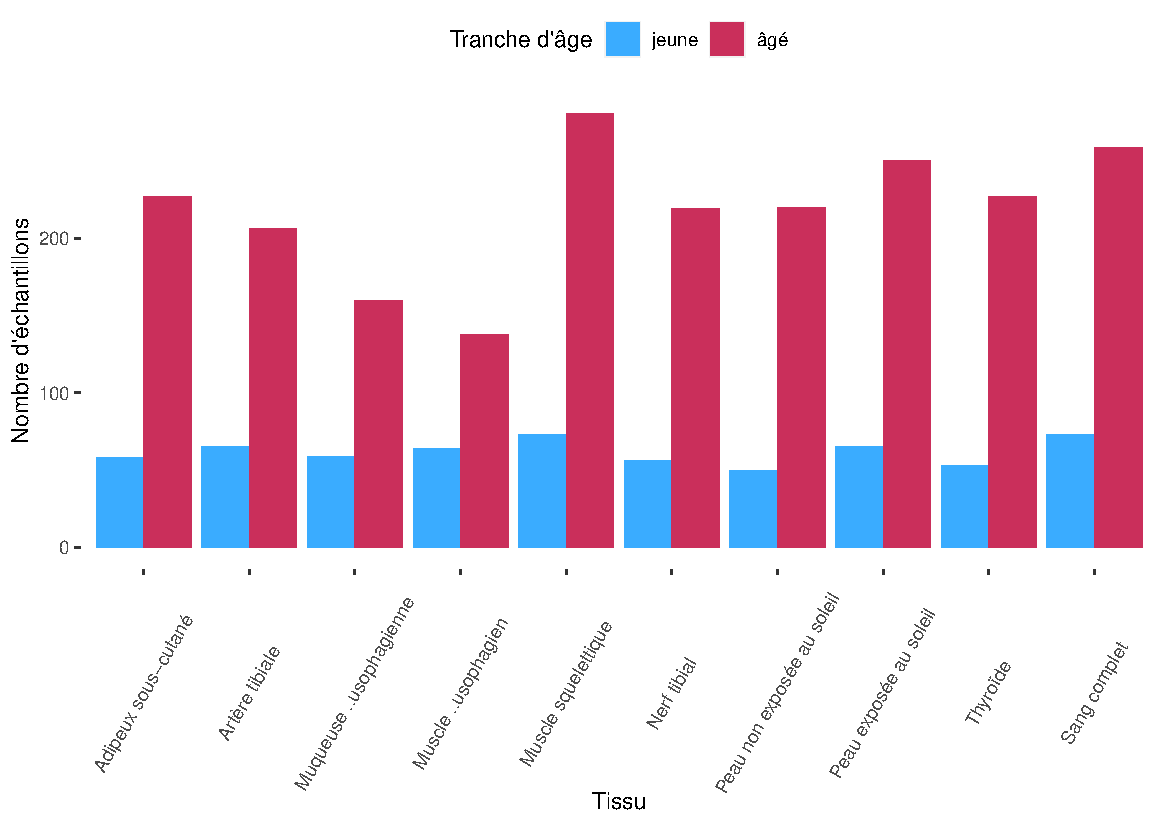
\includegraphics[width=0.8\textwidth]{img/chap2/chap2_sample_count_by_tissu_after_filter.pdf}
    \caption{Nombre d'échantillons disponibles par tissu dans les tranches d'âge jeune (20-30) et âgé (60-70) après filtration selon la cohorte et le statut cancéreux.}
    \label{figure:sample_count_by_tissu_after_filter}
\end{figure}

En plus de ces sélections de tissus, certains échantillons ont directement nécessité une filtration afin de prévenir de potentiels biais qui pourraient altérer l'analyse de co-expression ou l'interprétation des modules en étant issus. Ainsi, seuls les échantillons répondant au critère d'inclusion dans la cohorte "GTEx Analysis Freeze" ont été retenus en premier lieu (Figure \ref{figure:data_filters}. Cette cohorte atteste que les échantillons n'étaient pas :
\begin{itemize}
    \item issus de donneurs ayant des liens de parenté ou de donneurs avec des critères d'exclusion, par exemple des donneurs avec des duplications ou délétions chromosomiques
    \item affectés d'un syndrome tel que défini par la base de données OMIM \citeB{Hamosh2005}, hors maladies liées au vieillissement
    \item ayant effectué une chirurgie de ré-assignation sexuelle
\end{itemize}
% issus de donneurs ayant des liens de parenté ou de donneurs avec des critères d'exclusion, par exemple des donneurs avec des duplications ou délétions chromosomiques, affectés d'un syndrome tel que défini par la base de données OMIM \citeB{Hamosh2005} (ce qui n'inclue pas les maladies liées au vieillissement), ou encore ayant effectué une chirurgie de ré-assignation sexuelle. 

Par ailleurs, l'expression des tissus tumoraux a montré, dans des études préalables, des modèles d'expression génétique différents de ceux non tumoraux \citeB{Tang2017}. Par conséquent, les échantillons de ces donneurs ont également été supprimées ici ainsi que les échantillons dont le statut cancéreux était inconnu. La répartition finale des échantillons par tissu et par tranche d'âge est visible en Figure \ref{figure:sample_count_by_tissu_after_filter}.


\subsection{Filtre sur les gènes}

On a considéré comme base dans cette étude uniquement les gènes codants pour une protéine (d'après GENCODE 26) sur les autosomes. Pour continuer à éviter l'influence du sexe, on a également limité les gènes des gonosomes à ceux du chromosome X. Afin de limiter l'ajout de biais d'origine technique, on a également exclu les gènes dont le compte de lecture (en anglais \textit{count}) était inférieur à 6 dans la totalité des échantillons \citeB{Rocke2001}. Les gènes n'ayant aucune variation se sont vu retirés du jeu de données car leur apport à la co-expression aurait était nul et leur conservation aurait entraîné l'utilisation de ressources inutile. Ces filtres ayant été appliqués par tissu, le nombre de gènes restant varie d'un tissu à un autre avec en moyenne 18687 gènes contre initialement 19 312 (Figure \ref{figure:data_filters}).



\subsection{Correction des facteurs confondants}

À l'instar de l'analyse d'expression différentielle, l'analyse de co-expression différentielle nécessite des données biaisées au minimum pour une construction de réseau de qualité. Ces biais (ou facteurs confondants) peuvent être tant techniques que biologiques et vont entraîner une augmentation de la variation de façon artificielle. Le risque est alors de détecter une différence artificielle et de l'assumer comme expérimentalement pertinente alors qu'elle est en fait due aux biais. Dans le cas de la co-expression plus spécifiquement, ces biais peuvent entraîner des corrélations erronées mais qui semblent crédibles entre certains gènes. Elles altèrent alors la construction du réseau de co-expression et par la suite la détection des modules qui se base sur un découpage en modules via les corrélations. Ainsi, il est essentiel de corriger ces facteurs confondants au préalable de l'utilisation du package R GWENA \citeB{Lemoine2021Dec} sur les données comme on va le faire par la suite.

La complexité de la correction des facteurs confondants réside dans leur suppression sans pour autant altérer la distribution des données ou supprimer le signal expérimental d'intérêt, ici les variations dans le transcriptome dues à l'âge. 
% Il est également important avec l'utilisation de GWENA de veiller à ce que la correction n'altère pas la topologie d'invariance d'échelle qu'on retrouve dans les données de transcriptomique après construction d'un réseau de co-expression \citeB{Zhang2005a}. En effet, cela invaliderait la méthode de détection des modules ultérieure car celle-ci repose sur une méthode présupposant la présence d'une telle topologie pour fonctionner.
Il est également important avec l'utilisation de GWENA de veiller à ce que la correction n'altère pas la topologie d'invariance d'échelle (\textit{scale-free topology}) qu'on retrouve dans les réseaux de co-expression construits sur des données de transcriptomique \citeB{Zhang2005a}. Cette propriété assure que la distribution des degrés des nœuds suivent en fait une loi de puissance. Briser cette topologie perturberait la détection des modules dans le réseau car la méthode employée pour cela présuppose la présence d'une telle topologie pour fonctionner.

% \todo{Je me demande si ces 2 paragraphes plus haut ne devraient pas finir en intro de thèse}

% La base de données GTEx n'échappe pas aux biais \citeB{Parsana2019} et a même été étudiée sur le plan de la contamination \citeB{Nieuwenhuis2020}.
La base de données GTEx n'échappe pas aux biais \citeB{Parsana2019, Nieuwenhuis2020} et doit donc passer par cette étape sensible de correction des facteurs confondants dans le cadre de notre analyse de co-expression.
Malgré le progrès de techniques ciblées sur des facteurs confondants connus comme l'effet de lot, l'effet de centre de prélèvement, le sexe, le poids, etc., celles-ci ne sont pas capables de corriger pour des facteurs peu explicites ou diffus comme la classe sociale, l'alimentation, la façon de manipuler des techniciens, etc. La correction par composante principale (CP) vise à répondre à ce type de problématique et a montré de bons résultats selon une évaluation par validation de voies de signalisation au sain de modules détectés \citeB{Parsana2019}. Elle a également montré de meilleurs résultats que d'autres méthodes telles que la régression multiple, le taux exonique, ou encore le numéro d'intégrité d'ARN (\textit{RNA integrity number}, ou RIN). Fait important pour la co-expression en particulier, cette méthode conserve la propriété d'invariance d'échelle des données requise pour la construction des modules de co-expression dans notre méthode.


\begin{table}[h!]
\centering
\begin{tabular}{llll}
\multirow{2}{*}{\textbf{Tissu}} & \multirow{2}{*}{\textbf{\begin{tabular}[c]{@{}l@{}}Nombre de CP \\ corrigées\end{tabular}}} & \multicolumn{2}{l}{\textbf{Nombre d'échantillons}} \\ \cline{3-4} 
                                &                                                                                             & \textbf{Jeune}            & \textbf{Âgé}           \\ \hline
Adipeux sous-cutané             & 1                                                                                           & 58                        & 227                    \\
Artère tibiale                  & 3                                                                                           & 65                        & 206                    \\
Muqueuse œusophagienne          & 1                                                                                           & 59                        & 160                    \\
Muscle œusophagien              & 3                                                                                           & 64                        & 138                    \\
Muscle squelettique             & 5                                                                                           & 73                        & 281                    \\
Nerf tibial                     & 4                                                                                           & 56                        & 219                    \\
Peau non exposée au soleil      & 4                                                                                           & 50                        & 220                    \\
Peau exposée au soleil          & 3                                                                                           & 65                        & 250                    \\
Thyroïde                        & 3                                                                                           & 53                        & 227                    \\
Sang complet                    & 1                                                                                           & 73                        & 259                   
\end{tabular}
\caption{Résumé du nombre de composantes utilisées pour effectuer la correction de l'expression par tissu, ainsi que le nombre d'échantillons inclus dans chacun pour les deux tranches d'âge.}
\label{table:nb_PC_corr_and_samples_by_tissue}
\end{table}


Cependant, cette correction va également corriger l'âge qui est notre variable d'intérêt. Afin de conserver cette information tout en ayant un effet de correction par CP sur les autres facteurs confondants, on a donc ajusté la méthode estimant le nombre $n$ de CP par lequel corriger les jeux de données. Au lieu d'utiliser une procédure de permutation \citeB{Buja1992Oct}, l'estimation de $n$ s'est faite en deux étapes :
\begin{itemize}
    \item Un test de corrélation de chaque gène avec l'âge associé à chaque échantillon (donc patient) en fonction de différent $n$ PC corrigées donne une liste de gènes significativement associés à l'âge.
    \item Cette liste de gènes par $n$ PC corrigées est ensuite croisée avec deux bases de données de gènes connus comme étant associés au vieillissement : GenAge \citeB{DeMagalhaes2004} et Digital Aging Atlas \citeB{Craig2015}. Y sont alors compté le nombre de gènes significatifs recoupés.
\end{itemize}
Finalement, le $n$ de PC à corriger retenu est celui où le nombre de gènes significatifs est le plus haut dans chaque base de données. En cas de divergence de ce $n$ entre les bases de données, on a sélectionné la valeur la plus basse de $n$ afin de ne pas risquer de corriger l'âge (Table \ref{table:nb_PC_corr_and_samples_by_tissue}).


% \todo[inline]{Idée de figure : remplacer cette table ou en touts cas la partie nb composantes par un ensemble de mini histogrames avec les deux bdd en un, et en facet pour chaque tissu.}


\subsection{Construction du réseau, détection des modules et co-expression différentielle}

Une fois les données pré-traitée, nous avons généré un réseau de co-expression de gènes indépendamment sur chacun des 10 tissus et tranche d'âge à l'aide du package GWENA \citeB{Lemoine2021Dec}. Les paramètres spécifiés étaient ceux par défaut de la fonction \verb+build_net+ à l'exception de la corrélation qui était basée sur Spearman et du seuil d'ajustement de la loi de puissance fixé à 0,8. Dans chaque réseau de tissu, on a ensuite détecté le nombre de modules via la fonction \verb+detect_modules+ selon un seuil de coupe de l'arbre hiérarchique identique dans chaque tissu et une taille de module minimale fixée à 20 gènes. Chaque ensemble de modules a ensuite été testé à l'aide de la fonction \verb+compare_conditions+ par tissu entre les deux tranches d'âges pour identifier les modules préservés, modérément préservés et non préservés avec le vieillissement.

\subsection{Investigation des phénomènes communs ou spécifiques du vieillissement}

\begin{figure}[hb]
    \centering
    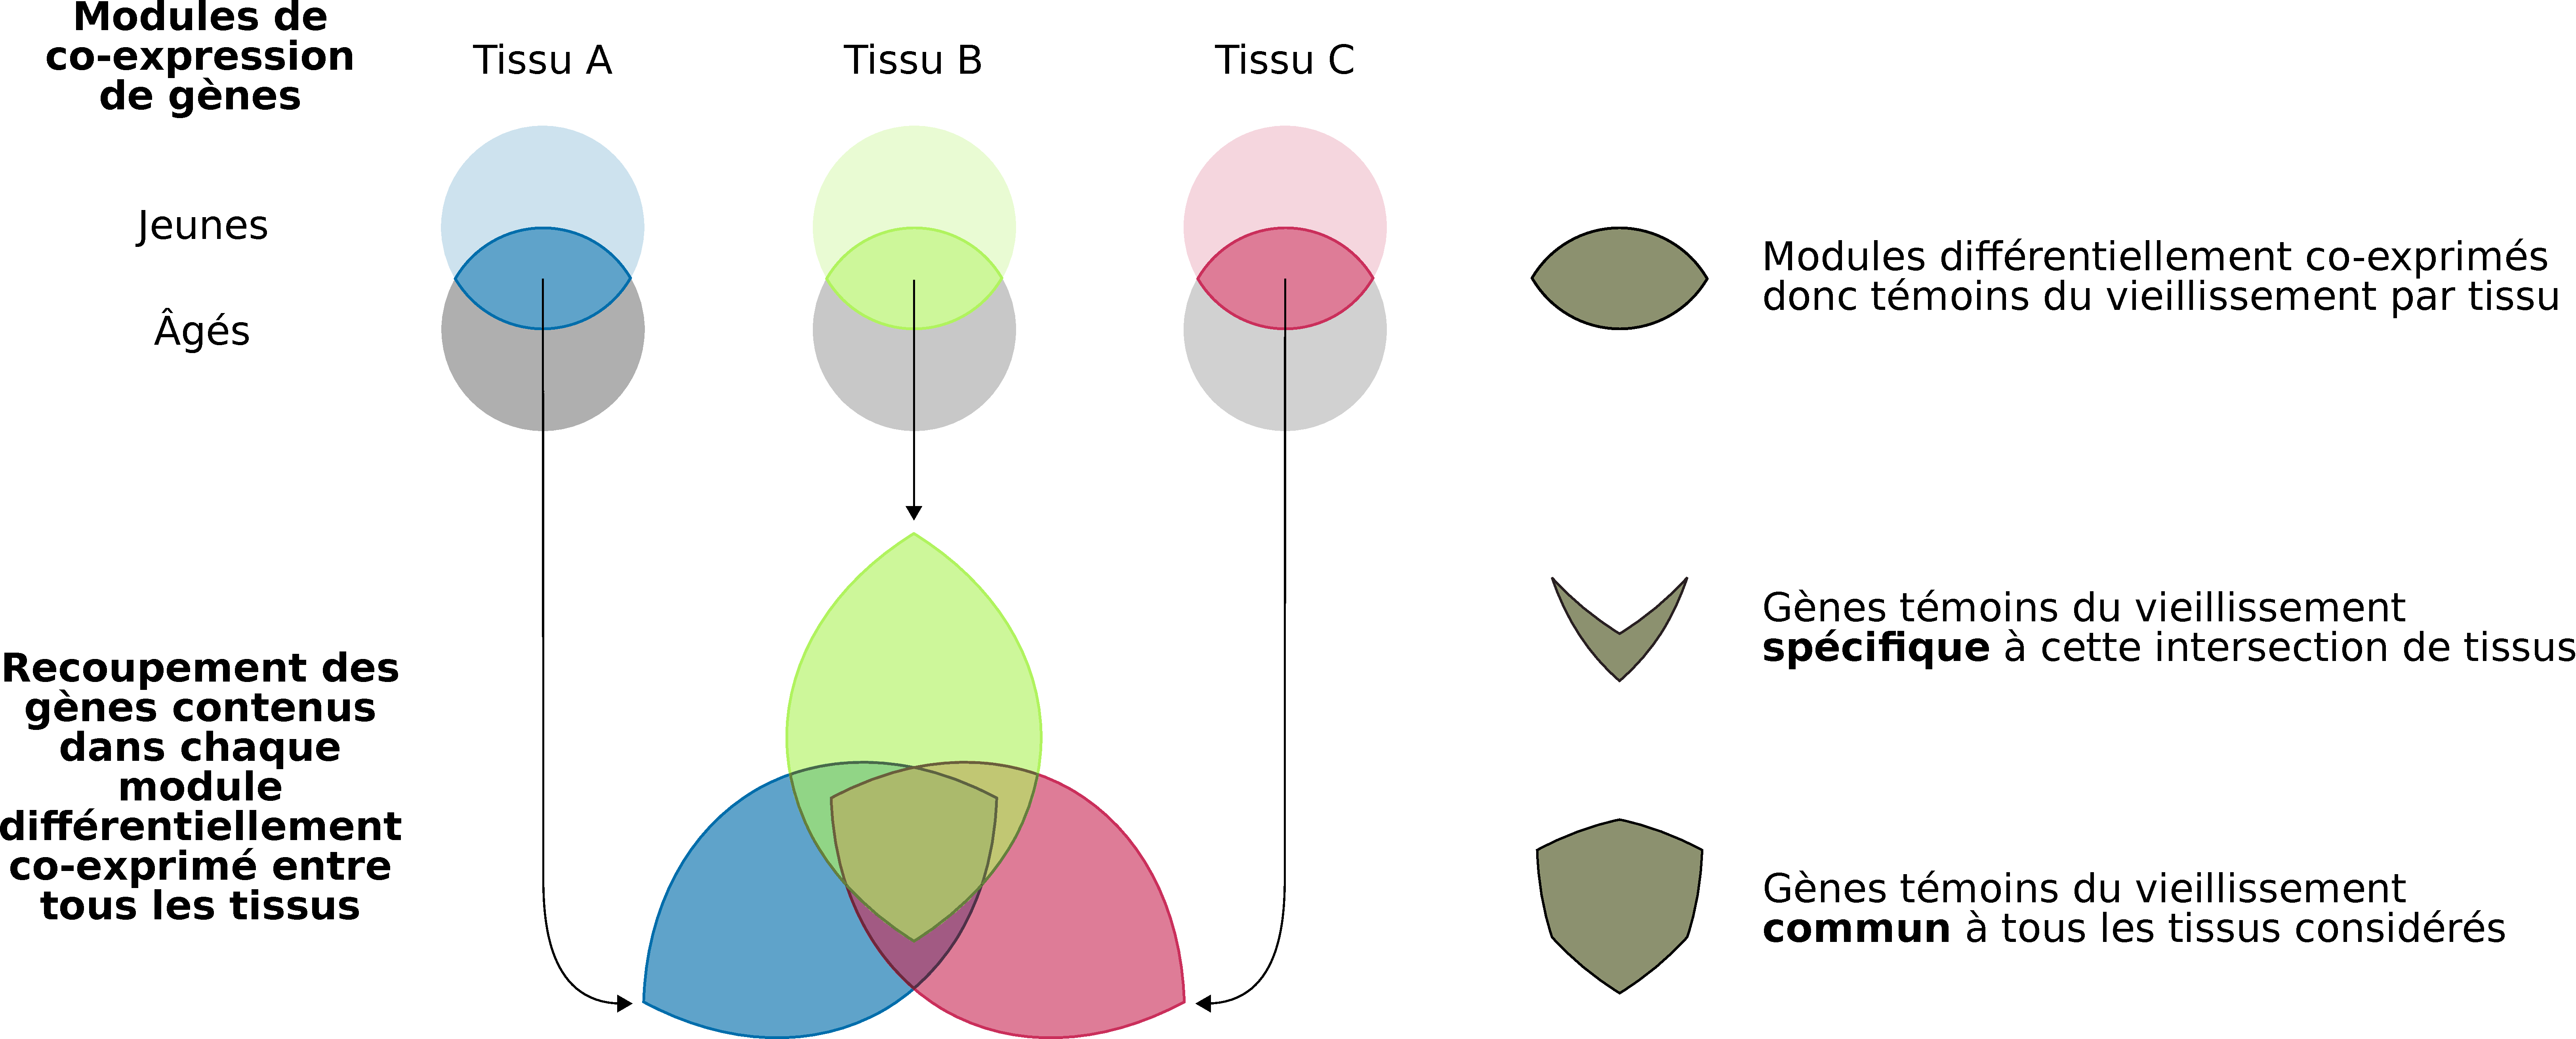
\includegraphics[width=1\textwidth]{img/chap2/chap2_intersection_explication.pdf}
    \caption{Schéma simplifié, avec trois tissus seulement, de la méthode de construction des intersections spécifiques et communes du vieillissement.}
    \label{figure:chap2_intersection_explication}
\end{figure}

Dans chaque tissu on a isolé les modules de co-expression modérément préservés (MP) et non préservés (NP) entre les deux tranches d'âge. On a ensuite effectué une intersection de leur contenu en gènes entre tous les tissus afin d'isoler les gènes participant à des phénomènes communs à plusieurs tissus et ceux participant à des phénomènes plus spécifiques d'un sous ensemble de tissus partageant des propriétés biologiques \ref{figure:chap2_intersection_explication}. Tous ont ensuite été enrichis via la fonction \verb+bio_enrich+ de GWENA et leurs résultats revus en regard de la littérature sur le vieillissement. Pour les plus pertinents d'entre eux, un résumé des termes Gene Ontology selon leur similarité sémantique a été réalisé à l'aide du package R rrvgo \citeB{rrvgo2021} qui reprend le principe de l'outil REVIGO \citeB{Supek2011Jul}.



\section{Résultats}

\subsection{Répartition des gènes en fonction de la tranche d'âge et du tissu}

\begin{figure}[!hb]
    \centering
    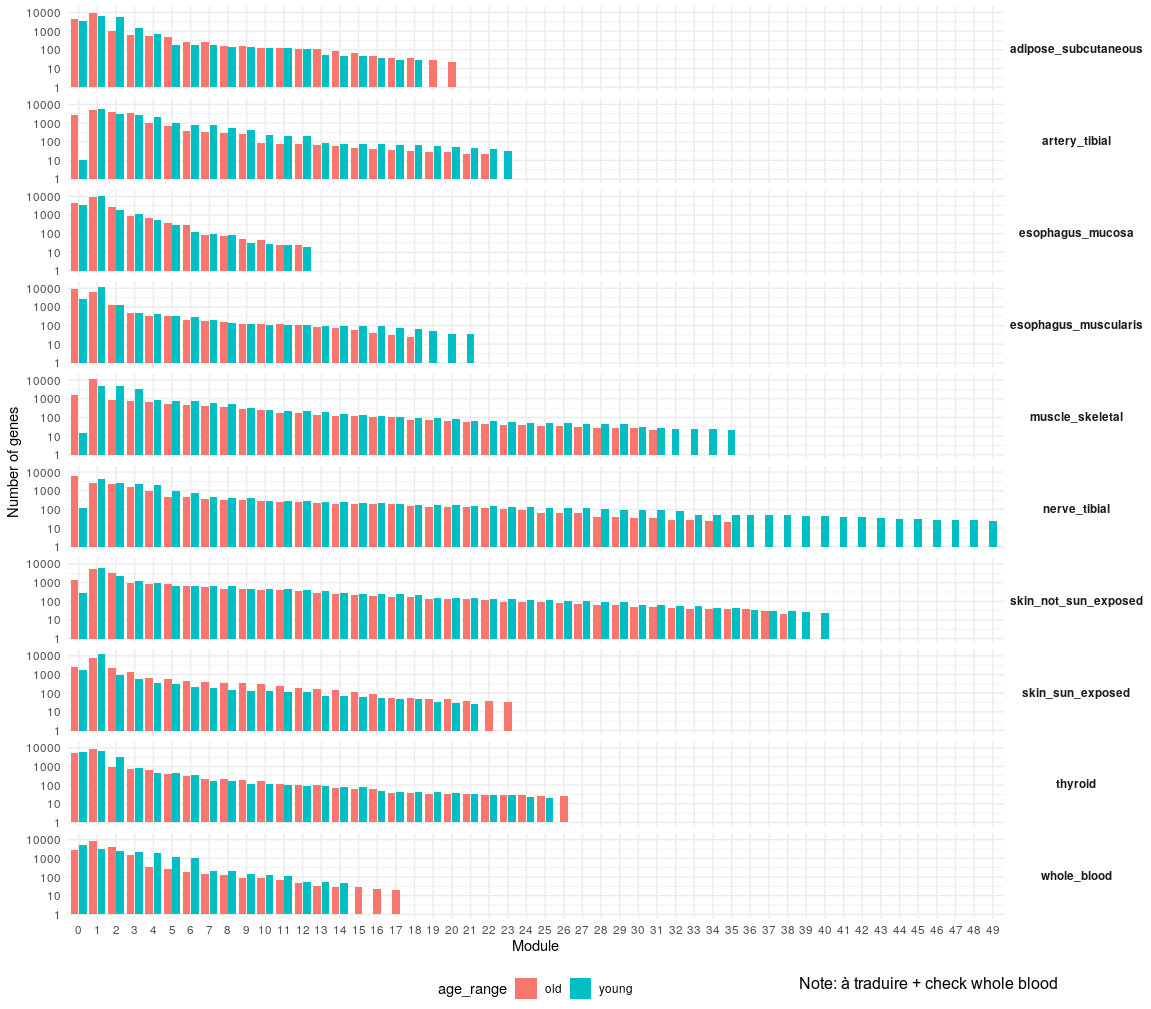
\includegraphics[width=0.95\textwidth]{img/chap2/chap2_repartition_genes_modules_tissus.png}
    \caption{Répartition des gènes (en échelle log10) pour chaque tissu entre les deux tranches d'âge jeune (bleu) et âgée (rouge)}
    \label{figure:repartition_genes_modules_tissus}
\end{figure}

La répartition des gènes entre les modules est hétérogène, tant entre les tranches d'âge qu'entre les tissus (Figure \ref{figure:repartition_genes_modules_tissus}), avec une moyenne à 26 modules tout confondu (25.2 pour les âgés et 26.8 pour les jeunes). Le module 0 présent sur la figure regroupe les gènes sans association à un module. Celui-ci est quasi systématiquement plus grand dans la tranche âgée que jeune, à l'exception des tissus de la thyroïde et du sang complet. Les tissus où cet écart est le plus creusé sont ceux disposant du plus grand nombre de modules dans la tranche d'âge jeune. Ces résultats sont cohérents avec la tendance à la perte de co-expression constatée dans les tranches d'âge âgées \citeB{Southworth2009} : la perturbation des voies de signalisation au cours du vieillissement entraîne une diminution de la co-expression entre gènes de ces voies.


\subsection{Modules spécifiques du vieillissement et recoupement inter-tissus}

Le but étant de rechercher des origines communes au vieillissement entre tous les tissus, on a ensuite effectué une étape de co-expression différentielle intra tissu. La tranche d'âge jeune a été prise pour référence, c’est-à-dire que le test indiquera si chaque module détecté dans la tranche d'âge jeune est préservé, modérément préservé, non préservé, ou non concluant. Les résultats ont été résumés en Table \ref{table:modules_status_all_tissues}. 

On y constate que certains tissus tendent à avoir proportionnellement moins de modules préservés lors du vieillissement. Avec moins de 50 \% de préservation on retrouve notamment le muscle œsophagien et squelettique, ainsi que de la peau exposée au soleil et la thyroïde. À cela s'ajoute que la peau exposée au soleil et le muscle squelettique sont les deux tissus ayant le plus de modules non préservés proportionnellement à leur nombre de modules.

\begin{table}[!ht]
\resizebox{\textwidth}{!}{
\begin{tabular}{llllllllll}
\multirow{2}{*}{\textbf{Tissu}} & \multicolumn{2}{l}{\textbf{Préservé}} & \multicolumn{2}{l}{\textbf{Modérement préservé}} & \multicolumn{2}{l}{\textbf{Non préservé}} & \multicolumn{2}{l}{\textbf{Non concluant}} & \textbf{Total} \\ \cline{2-10} 
                                & \textbf{\#}       & \textbf{\%}       & \textbf{\#}             & \textbf{\%}            & \textbf{\#}         & \textbf{\%}         & \textbf{\#}          & \textbf{\%}         & \textbf{\#}    \\ \hline
Adipeux sous-cutané             & 12                & 67              & 4                       & 22                   & 0                   & 0                 & 2                    & 11               & 18             \\
Artère tibiale                  & 13                & 57              & 8                       & 35                   & 1                   & 4                 & 1                    & 4                & 23             \\
Muqueuse œusophagienne          & 3                 & 25              & 8                       & 67                   & 1                   & 8                 & 0                    & 0                & 12             \\
Muscle œusophagien              & 9                 & 43              & 6                       & 29                   & 0                   & 0                 & 6                    & 29               & 21             \\
Muscle squelettique             & 14                & 40              & 13                      & 37                   & 5                   & 14                & 3                    & 9                & 35             \\
Nerf tibial                     & 35                & 71              & 9                       & 18                   & 1                   & 2                 & 4                    & 8                & 49             \\
Peau non exposée au soleil      & 36                & 90              & 4                       & 10                   & 0                   & 0                 & 0                    & 0                & 40             \\
Peau exposée au soleil          & 10                & 48              & 8                       & 38                   & 2                   & 10                & 1                    & 5                & 21             \\
Thyroïde                        & 12                & 48              & 8                       & 32                   & 1                   & 4                 & 4                    & 16               & 25             \\
Sang complet                    & 9                 & 64              & 4                       & 29                   & 0                   & 0                 & 1                    & 7                & 14              
\end{tabular}
}
\caption{Nombre (\#) et ratio (\%) de modules par statut de préservation selon chaque tissu.}
\label{table:modules_status_all_tissues}
\end{table}


Afin d'observer des similarités de mécanismes du vieillissement entre ces différents tissus, on a dans un premier temps regardé si des gènes communs existaient entre les modules modérément préservés (MP) et non  préservés (NP). Le diagramme UpSet \citeB{Lex2014} visible en Figure \ref{figure:upset_intersection_genes_tissu_unpres_modpres} permet de constater le faible recouvrement entre les gènes contenus dans les modules MP et NP. Ce diagramme révèle également que le maximum de tissus avec des gènes communs est 5. Ce chiffre est à mettre en contraste avec le fait que les modules créés par GWENA pour un même tissu ne sont pas chevauchant. Un gène classé dans un module ne sera donc pas également classé dans un autre et on aurait pu espérer une intersection au maximum de taille 10 étant donné qu'on dispose de 10 tissus. 

\begin{landscape}
\begin{figure}[p]
  \centering
  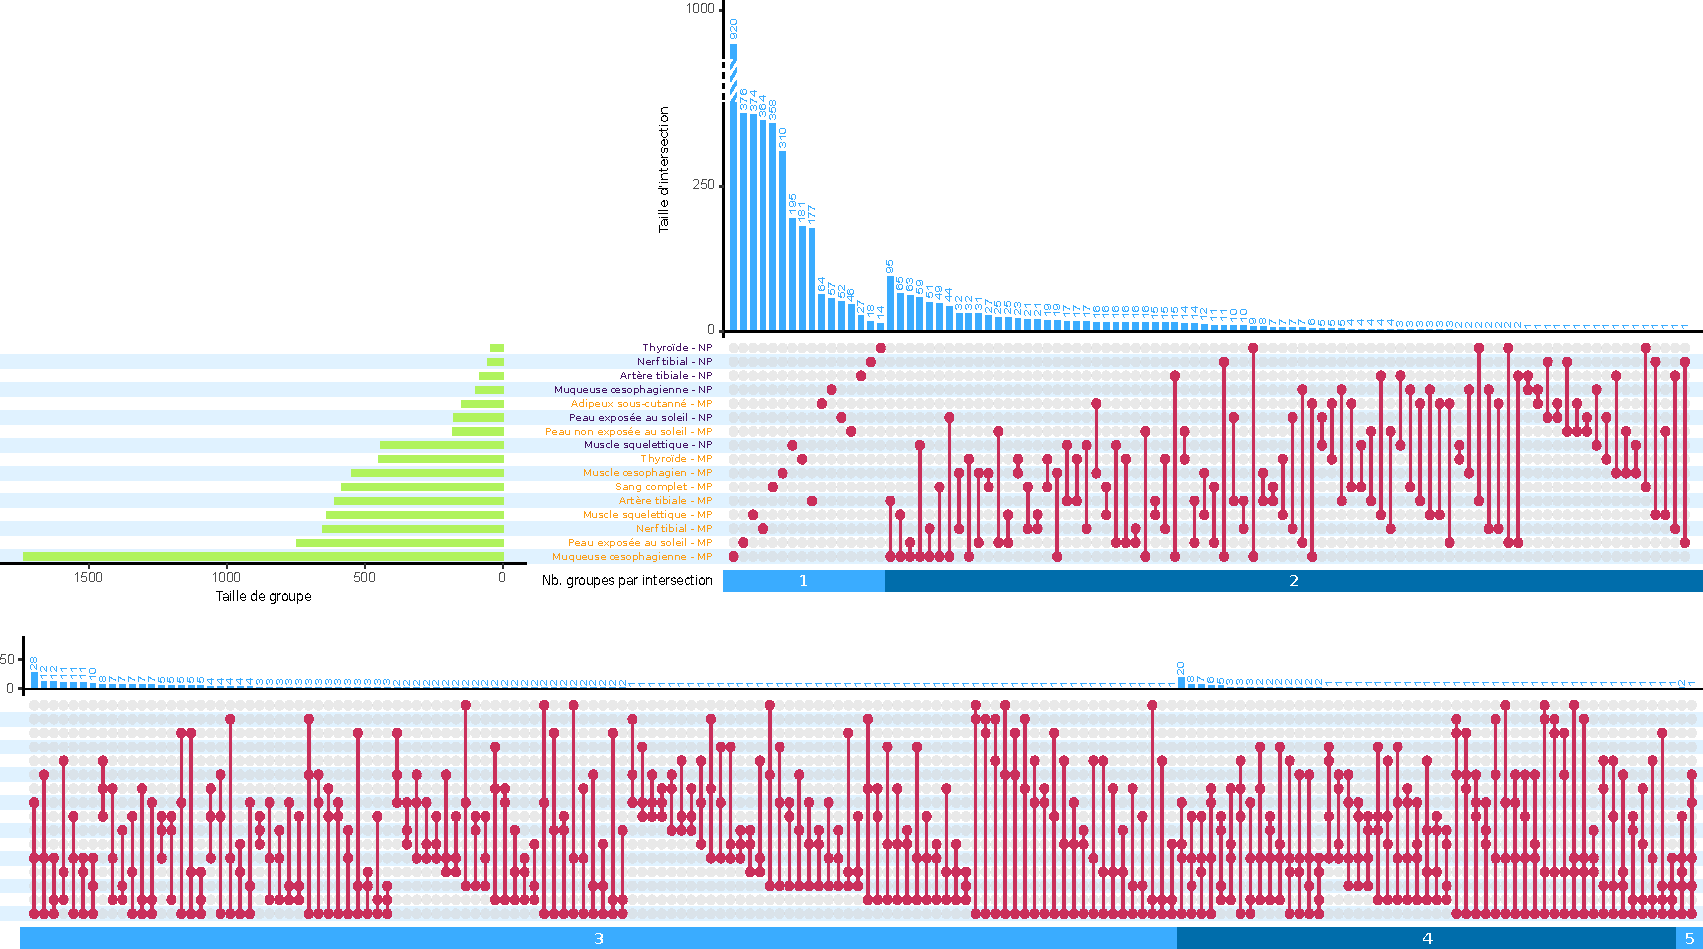
\includegraphics[width=1.5\textheight]{img/chap2/chap2_upset_genes_unpres_modpres_by_tissue.pdf}
  \caption[Intersections entre tous les jeux de gènes pour chaque couple tissu / statut de préservation]{Intersections entre tous les jeux de gènes pour chaque couple tissu / statut de préservation. Le diagramme Upset est une représentation qui vise à remplacer une visualisation par diagramme de Venn, ce dernier n'étant pas adaptée à la représentation de plus de 5 catégories. La matrice d'intersection (en orange) indique quel couple tissu / statut est considéré dans l'intersection (rose si pris en compte, gris si non) et quels sont les autres tissus dans cette intersection (ligne rose). L'histogramme des tailles de groupe (gris) à gauche de la matrice indique le nombre total de gène contenu dans le couple tissu / statut en ligne. L'histogramme des tailles d'intersection indique le nombre de gènes contenu dans l'intersection indiquée en matrice d'intersection pour cette colonne.}
  \label{figure:upset_intersection_genes_tissu_unpres_modpres}
\end{figure}
\end{landscape}

En plus de ce nombre maximal de tissus présent dans une intersection, certains tissus vont se retrouver plus fréquemment dans ces intersections en raison de leur nombre de modules MP/NP ou de modules contenant plus de gènes (Table \ref{table:modules_status_all_tissues}). Ainsi, les modules MP de la muqueuse œsophagienne regroupent 1750 gènes et tendent à se positionner dans plus d'intersection que la moyenne. Une séparation est toutefois visible entre les deux types de statut MP et NP dans les intersections au-delà de 2 tissus et avec un minimum de trois gènes.


\subsection{Répartition des phénomènes communs liés au vieillissement dans plusieurs tissus}

\begin{table}[hb]
\centering
\resizebox{0.8\textwidth}{!}{
\begin{tabular}{@{}lllllllllll@{}}
\rotatebox{90}{\textbf{Muqueuse œusophagienne}}   & \rotatebox{90}{\textbf{Artère tibiale}}                      & \rotatebox{90}{\textbf{Thyroïde}}                 & \rotatebox{90}{\textbf{Muscle squelettique}}      & \rotatebox{90}{\textbf{Peau exposée au soleil}}   & \rotatebox{90}{\textbf{Muscle œusophagien}}       & \rotatebox{90}{\textbf{Nerf tibial}}              & \rotatebox{90}{\textbf{Peau non exposée au soleil}} & \rotatebox{90}{\textbf{Adipeux sous-cutané}}      & \rotatebox{90}{\textbf{Sang complet}}             & \textbf{Phénomène du vieillissement observé}       \\ \midrule
\cellcolor[HTML]{F8A102} & \cellcolor[HTML]{F8A102}            &                          & \cellcolor[HTML]{F8A102} &                          &                          &                          & \cellcolor[HTML]{F8A102}   &                          &                          & Homéostasie                               \\
                         & \cellcolor[HTML]{F8A102}            & \cellcolor[HTML]{F8A102} &                          &                          & \cellcolor[HTML]{F8A102} &                          &                            &                          &                          & Régulation de la transcription            \\
\cellcolor[HTML]{F8A102} &                                     & \cellcolor[HTML]{F8A102} & \cellcolor[HTML]{F8A102} &                          &                          &                          &                            &                          &                          & Dérivés réactifs de l'oxygène - peroxydes \\
                         &                                     & \cellcolor[HTML]{F8A102} &                          & \cellcolor[HTML]{F8A102} & \cellcolor[HTML]{F8A102} & \cellcolor[HTML]{F8A102} &                            &                          &                          & Dérivés réactifs de l'oxygène - dGTP      \\
                         &                                     & \cellcolor[HTML]{F8A102} &                          &                          &                          &                          & \cellcolor[HTML]{F8A102}   & \cellcolor[HTML]{F8A102} &                          & Inflammation                              \\
                         &                                     &                          &                          & \cellcolor[HTML]{F8A102} & \cellcolor[HTML]{F8A102} & \cellcolor[HTML]{F8A102} &                            &                          &                          & Désamination                              \\
\cellcolor[HTML]{F8A102} & \cellcolor[HTML]{F8A102}            &                          &                          &                          &                          & \cellcolor[HTML]{F8A102} &                            &                          &                          & Coagulation - plaquettes                  \\
\cellcolor[HTML]{F8A102} & \cellcolor[HTML]{F8A102}            & \cellcolor[HTML]{F8A102} &                          &                          &                          & \cellcolor[HTML]{F8A102} &                            &                          &                          & Coagulation - global                      \\
\cellcolor[HTML]{F8A102} & \cellcolor[HTML]{F8A102}            &                          & \cellcolor[HTML]{F8A102} &                          &                          &                          &                            &                          &                          & Méthylation - folate, B12, selenium       \\
                         &                                     &                          & \cellcolor[HTML]{F8A102} & \cellcolor[HTML]{F8A102} &                          &                          &                            & \cellcolor[HTML]{F8A102} &                          & Méthylation - déméthylase                 \\
\cellcolor[HTML]{F8A102} & \cellcolor[HTML]{F8A102}            &                          & \cellcolor[HTML]{F8A102} &                          &                          &                          &                            &                          & \cellcolor[HTML]{F8A102} & Altération de la MEC                      \\
                         &                                     & \cellcolor[HTML]{F8A102} &                          & \cellcolor[HTML]{F8A102} & \cellcolor[HTML]{F8A102} &                          &                            &                          &                          & Anomalie du taux de glutamine             \\
\cellcolor[HTML]{F8A102} &                                     &                          &                          & \cellcolor[HTML]{F8A102} &                          &                          & \cellcolor[HTML]{F8A102}   &                          &                          & Synthèse de pigment (dont mélanine)      \\
\cellcolor[HTML]{F8A102} & \cellcolor[HTML]{F8A102}            & \cellcolor[HTML]{F8A102} & \cellcolor[HTML]{F8A102} &                          &                          &                          &                            &                          &                          & Anomalie du taux de fer                   \\
\midrule
8                        & 7                                   & 7                        & 6                        & 5                        & 4                        & 4                        & 3                          & 2                        & 1                        & \textbf{Total}                   
\end{tabular}
}
\caption[Phénomènes connus dans le vieillissement et observés dans les intersections de modules MP et NP pour chaque tissu]{Phénomènes connus dans le vieillissement et observés dans les intersections de modules MP et NP pour chaque tissu. Les modules MP et NP ont été joints par tissus et les tissus ont été ordonnés par nombre décroissant de phénomènes du vieillissement présent. MEC : Matrice extra-cellulaire.}
\label{table:intersection_aging_global_phenomenons}
\end{table}


Pour mieux comprendre les fonctions physiologiques communes en jeu et pouvant être impliquées dans le vieillissement, les intersections de plus de 3 tissus et ayant au moins 5 gènes ont été enrichies via GWENA. Comme visible en Annexe \ref{annexe:chap_2_genes_intersect_enrichments} dans les tables des enrichissements obtenus, 5 intersections n'ont pas donné d'enrichissement significatif malgré un nombre de gènes équivalent à d'autres intersections avec enrichissement. Les 18 autres intersections ont quant à elles retourné des fonctions physiologiques (Gene Ontology \citeB{Ashburner2000}, CORUM \citeB{Ruepp2008}) et voies d'activation (KEGG \citeB{Kanehisa2019}, REACTOME \citeB{Fabregat2016}, WikiPathways\citeB{Slenter2018}) connues comme faisant partie du vieillissement global, ou de manifestations spécifiques à plusieurs tissus. Ainsi on retrouve, dans ces intersections de modules peu ou pas préservés dans la tranche âgée, des fonctions associées à l'homéostasie, la régulation de la transcription, la gestion des dérivés réactifs de l'oxygène, l'inflammation, etc. (Table \ref{table:intersection_aging_global_phenomenons} et Figure \ref{figure:revigo_resume_4_enrich}). La muqueuse œsophagienne bien qu'ayant un nombre de gènes plus élevé que les autres tissus ne se retrouve pas sur-représentée dans ces phénomènes observés. Cela indique donc que la majorité de ses gènes se trouvent dans les intersections de faible taille, tant en gènes qu'en nombre de tissus recoupés. Le sang complet, le tissu adipeux sous-cutané et la peau non exposée au soleil sont eux les tissus les moins présents dans ces intersections avec des phénomènes liés au vieillissement. Le sang complet est notablement absent des intersections avec des phénomènes liés à la coagulation. Les tissus ayant un fort renouvellement (voir en Table \ref{table:tissu_telomere_effet}) que sont les épithéliums (peau exposée au soleil, artère tibiale, muqueuse œsophagienne) sont porteurs d'un grand nombre de phénomènes, ainsi que la thyroïde et le muscle squelettique. 


\begin{figure}[ht]
    \centering
    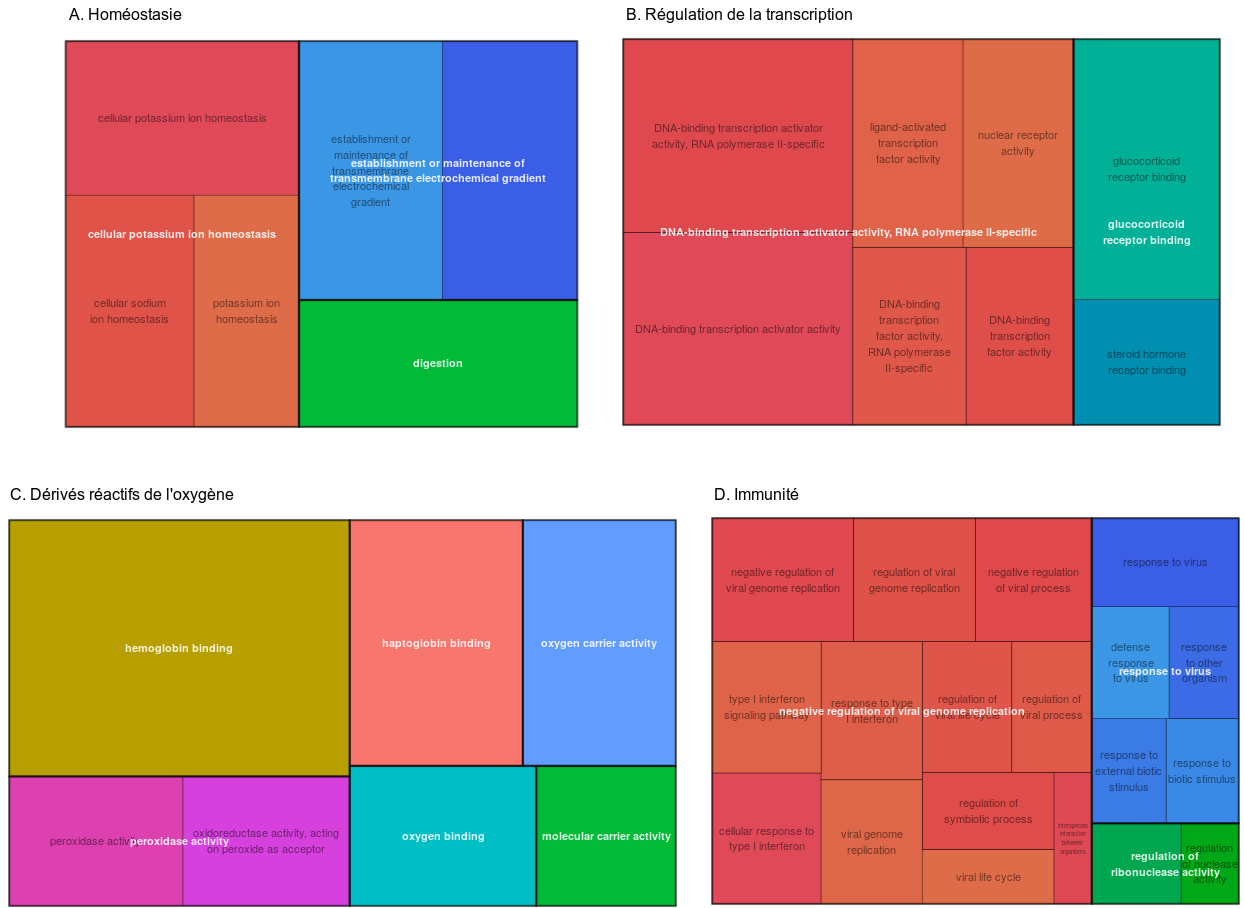
\includegraphics[width=1\textwidth]{img/chap2/chap2_revigo_resume_4_enrich.png}
    \caption[Exemple de résumé des enrichissements sur GO pour 4 des intersections par carte proportionnelle]{Exemple de résumé des enrichissements sur GO pour 4 des intersections par carte proportionnelle. Chaque ensemble de GO terme partageant une ontologie parente commune (selon un score de similarité) est groupé sous une même couleur. Chaque carte présente ici un phénomène connu dans le vieillissement : A. Homéostasie (GO \textit{Biological Process}), B. Régulation de la transcription (GO \textit{Biological Process}), C. Dérivés réactifs de l'oxygène (GO \textit{Molecular Function}), D. Inflammation (GO \textit{Biological Process}) }
    \label{figure:revigo_resume_4_enrich}
\end{figure}

Des anomalies phénotypiques ont été relevées (via enrichissement sur HPO \citeB{Kohler2019}) et présentent un lien parfois direct avec les altérations physiologiques précédemment relevées, et parfois plus éloigné car issues d'une chaine d'événements et réactions physiologiques. 
À ces anomalies du taux de fer détectés dans les fonctions physiologiques coïncident ainsi des phénotypes d'anémie (déficience en taux de globules rouges ou en concentration d'hémoglobine) ou de défaut de coagulation avec hémorragies diverses (épistaxis, saignement gingival, menstruations hors cycle, hémorragie cérébrale). De même, les tissus présentant une altération de la matrice extra-cellulaire (MEC) ont été associés avec des taux élevés de protéine C-réactive et d'anomalies de la fonction exocrine du pancréas ainsi que de malabsorption des lipides et ce qui en découle (stéatorrhée, pancréatite, thrombose veineuse). Ces résultats confirment le lien entre vieillissement et dérèglement progressif de l'homéostasie entrainant en cascade des pathologies de trouble de la coagulation \citeB{Franchini2006,Kario1993} et de la dégradation des lipides circulants \citeB{Yamamoto2014, Hirschfield2003}. Cependant d'autres résultats semblent moins intuitifs comme dans le cas de pathologies liées au sexe (azoospermie, maladie d'hérédité gonosomale) relevées parallèlement à la déméthylation dans le tissu adipeux, le muscle squelettique et la peau non exposée au soleil. Ces informations, en l'absence d'erreur technique, semblent continuer de montrer la complexité des relations entre pathologies et vieillissement.

Enfin, on a exploré le vieillissement et son phénomène de perturbation de la régulation de la transcription en évaluant l'enrichissement d'éléments de régulation (MiRTarBase \citeB{Chou2018}, TRANSFAC \citeB{Matys2006}). L'intersection présentant des phénomènes de coagulation globale est ainsi fortement enrichi en micro ARN (miARN). Ceux-ci contiennent notamment des miARN associés aux 3 gènes de la génération de fibrinogène FGA, FGB, FGG comme détectés lors du chapitre précédent. Quelques autres intersections. Deux facteurs de transcription (FT), HNF1A et HNF1B, sont également significatifs bien que normalement exprimés dans le foie. Cela s'explique par la production de facteurs de la coagulation (dont FGA, FGB, FGG) dans celui-ci et un effet connu de l'altération de production de ces facteurs dans le cadre d'une perturbation de l'expression de HNF1A et HNF1B \citeB{Costa2003}. L'intersection associée à l'inflammation quant à elle ne présente qu'un seul miARN agissant ici sur RSAD2, IFI44, OASL, et EPSTI1 présents dans l'intersection. RSAD2 et OASL sont également connus pour être stimulé par des interférons de type I (\textalpha{} et \textbeta{}) qui ont entre autres IRF1 (pour \textit{interferon related factor 1}) pour FT \citeB{Schoggins2011}. Ce facteur IRF1 fait par ailleurs parti de la liste des FT détectés dans cette intersection. On y trouve un large panel d'autres membres de la famille d'IRF (de 1 à 9 à l'exception d'IRF6) dont l'implication dans l'inflammation s'exerce tant dans la réaction innée qu’acquise \citeB{Frisch2020}. Mais tous les FT détectés via enrichissement n'étaient pas des IRF. Bien que n'étant pas directement liés à la régulation des interférons, STAT2 est présent dans la voie de signalisation des interférons \textalpha{} et \textbeta{} détecté plus tôt (R-HSA-909733). Le dernier FT identifié, FOXP1, n'est quant à lui pas contenu dans cette voie, mais agit sur l'engagement des cellules souches mésenchymateuses et la sénescence au cours du vieillissement \citeB{Infante2018} et sur de la régulation d'autres cytokines, l'interleukine 1 et 12 d'après UniprotKB (Q9H334).

\begin{figure}[p]
    \centering
    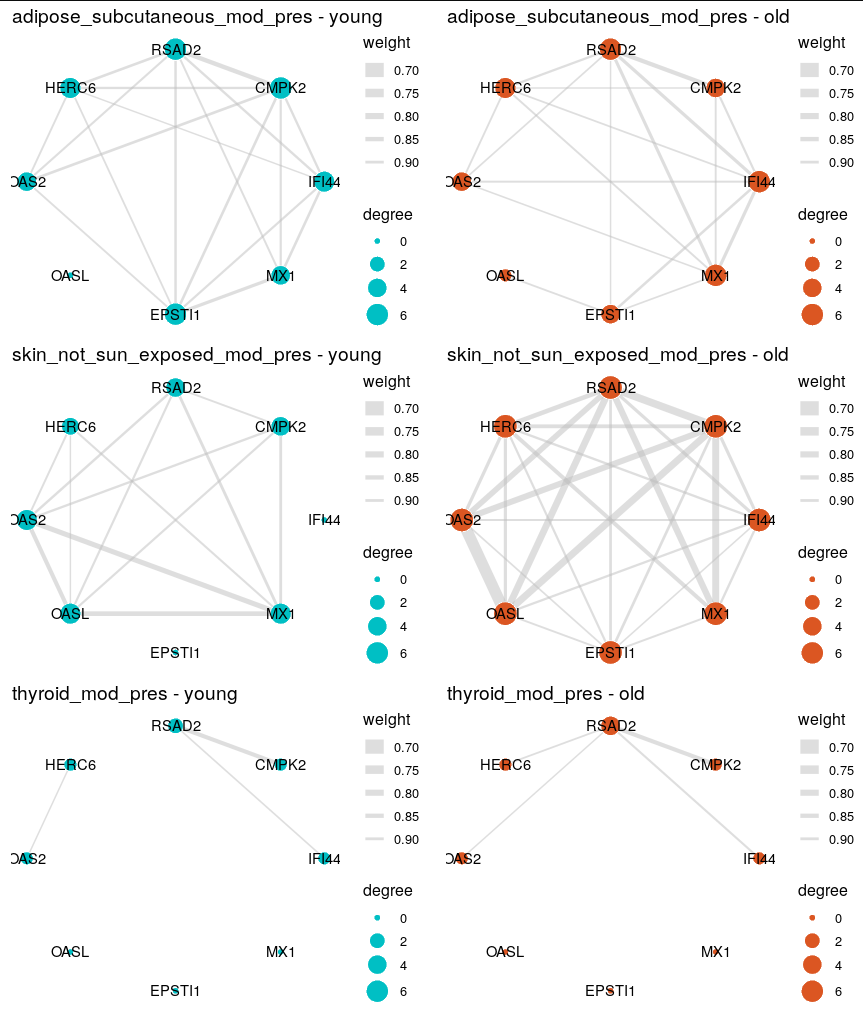
\includegraphics[width=1\textwidth]{img/chap2/chap2_graphs_intersection_plot_adipo_skinnosun_thyr.png}
    \caption[Réseaux de co-expression des gènes de l'intersection associée au phénomène d'inflammation lors du vieillissement entre les deux tranches d'âge]{Réseaux de co-expression des gènes de l'intersection associée au phénomène d'inflammation lors du vieillissement entre les deux tranches d'âge. Le réseau est filtré à 0.95 de dissimilarité (sur une échelle de 0 à 1) pour des questions de lisibilité et 3 tissus sont présentés : tissu adipeux, peau non exposée au soleil et thyroïde.}
    \label{figure:graphs_intersection_plot_adipo_skinnosun_thyr}
\end{figure}


\subsection{Les variation de co-expression dans l'intersection liée à l'inflammation}

L'inflammation systémique chronique de faible intensité est une des marques connues du vieillissement \citeB{Lopez-Otin2013, Franchini2006}. La complexité des mécanismes d'immunité et d'inflammation rend ce phénomène particulièrement difficile à étudier et les publications actuelles tendent donc à cibler peu d'acteurs en même temps (gène, protéine, miARN, etc.) et à se concentrer sur des contextes très précis \citeB{Franceschi2017}. Bien qu'apportant un niveau de preuve inférieur à toute validation expérimentale, les réseaux de co-expression de gènes permettent de comprendre bien plus d'acteurs. À titre d'exemple, on a souhaité ici détailler le cas de l'intersection de gènes associés à l'inflammation lors du vieillissement (Figure \ref{figure:revigo_resume_4_enrich}.D).


Les variations de motif dans la co-expression sont bien souvent la première cause de non-préservation des modules \citeB{Ritchie2016}. Des changements de score de centralité, des modifications de gène pivot (\textit{hub gene}), des suppressions totales de signal sont bien souvent à l'origine de cette différence de topologie détectée entre les modules à l'aide de la co-expression différentielle \citeB{Ritchie2016,Zhang2005a}. Cet effet se manifeste de plusieurs façons dans le cas de l'intersection sur l'inflammation comme visible en figure \ref{figure:graphs_intersection_plot_adipo_skinnosun_thyr}. Bien que la variation de la co-expression ne soit pas identique entre tous les tissus qui forment cette intersection, on observe des acteurs communs. Le gène RSAD2 précédemment mis en avant comme gène simulé par le FT IRF1 et un mARN devient ainsi un gène pivot dans la condition âgée selon le classement de score de centralité. Cependant, les sources de progression dans le classement selon la centralité divergent selon le tissu. Dans le tissu adipeux on constate que c'est dû à un renfort de la co-expression entre RSAD2 et IF44 associé à une perte partielle de co-expression globale par CMPK2, gène pivot dans la condition jeune. Dans la peau non exposée au soleil, on constate un renfort global de la co-expression avec toutefois une centralisation vers RSAD2. Une augmentation localisée entre OAS2 et OASL est également à noter. Enfin, dans la thyroïde, c'est une déconnexion entre HERC6 et OAS2 au profit de RSAD2 qui le rend gène pivot dans la condition âgée. Si cette réorganisation de la co-expression vers RSAD2 aurait pu être issue d'une contribution d'IRF1 ou tout autre IRF étant donné les informations précédentes, des analyses complémentaires ont précisé qu'aucun des IRF détectés comme FT auparavant n'était présent dans le module où se trouve RSAD2 (jeune comme âgé). L'origine de la variation de RSAD2 et OAS2/OASL pourrait donc être d'une autre nature qu'une modification de la transcription d'un ou plusieurs FT.

\begin{figure}[p]
    \centering
    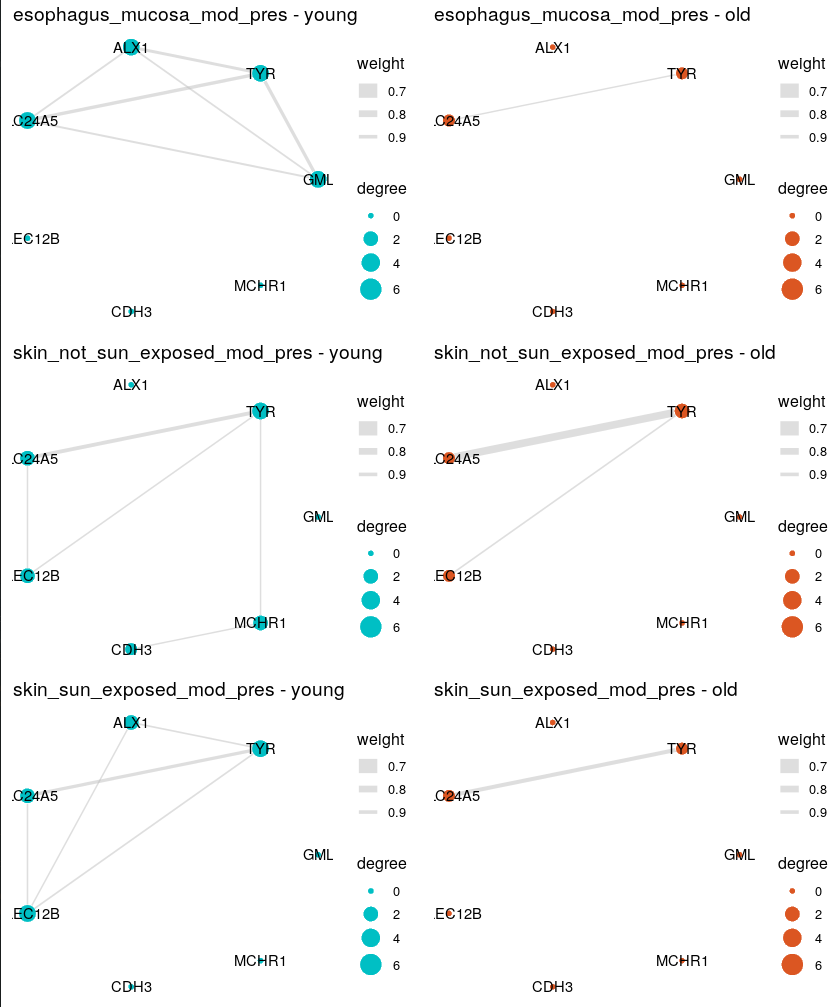
\includegraphics[width=1\textwidth]{img/chap2/chap2_graphs_intersection_melanine.png}
    \caption[Réseaux de co-expression des gènes de l'intersection associée à la surproduction de mélanine lors du vieillissement entre les deux tranches d'âge]{Réseaux de co-expression des gènes de l'intersection associée à la surproduction de mélanine lors du vieillissement entre les deux tranches d'âge. Le réseau est filtré à 0.99 de dissimilarité (sur une échelle de 0 à 1) pour des questions de lisibilité et 3 tissus sont présentés : muqueuse œsophagienne, peau non exposée au soleil et peau exposée au soleil.}
    \label{figure:graphs_intersection_melanine}
\end{figure}


\subsection{Cas particulier : le vieillissement spécifique à la peau}

Si le vieillissement partage des mécanismes et altérations communes à travers plusieurs tissus, il existe parallèlement des altérations spécifiques à certains tissus. Bien que ne permettant pas l'enrichissement global de la compréhension du vieillissement, ces altérations locales nécessitent de s'y intéresser afin de prévenir et prendre en charge les pathologies qui s'y rattachent. En étudiant les intersections ne présentant pas d'enrichissements liés aux mécanismes communs du vieillissement et en tenant compte des tissus inclus, on peut ainsi étudier l'impact du vieillissement spécifique du tissu.
% La peau est un des organes dont l'intégrité est la plus susceptible d'être mise à mal par le vieillissement en raison de son exposition directe avec l'environnement extérieur. 
% Le premier facteur de vieillissement extrinsèque est le photo-vieillissement dont les effets sont cumulatifs avec le temps \citeB{Farage2008}. Il se caractérise majoritairement pas une exposition aux UVs (UVA et UVB) qui vont induire des détériorations des fibres de collagène et d'élastine dans la peau. À noter également, des altérations de la matrice extra-cellulaire entre l'épiderme et le derme qui sont les deux couches composant la peau \citeB{Rogowski-Tylman2016}. 

% Une intersection faite de la peau exposée au soleil, la peau non exposée au soleil et la muqueuse œsophagienne fait état dans notre cas d'un tel type de photo-vieillissement. 
Une intersection faite de la peau exposée au soleil, la peau non exposée au soleil et la muqueuse œsophagienne fait état dans notre cas d'un tel type de vieillissement. 
Elle est en effet composée principalement d'enrichissements sur des fonctions physiologiques directement liées à la synthèse et régulation de mélanine comme exposé en Figure \ref{figure:revigo_resume_melanine}.
% Ce pigment synthétisé par les mélanocytes à partir d'une oxydation de la tyrosine joue un rôle majeur de lutte contre les dégâts provoqués par les UV \citeB{Bettley1965}. 
C'est le gène TYR, impliqué dans cette synthèse qu'on trouve dans le réseau de co-expression de notre intersection qui entraîne notamment cet enrichissement. Il est détecté comme gène pivot (score de centralité) dans chacun des tissus et chacune des tranches d'âge (Figure \ref{figure:graphs_intersection_melanine}), attestant ainsi de son rôle majeur dans la régulation de la mélanogénèse. On constate qu'il est lié dans la condition jeune par une relation forte (dissimilarité < 0.8 en moyenne) avec un autre gène, SLC24A5. Ce gène est connu pour coder pour un échangeur de cations (sodium, potassium, calcium) de façon générale et a été plusieurs fois soupçonné d'une contribution à la régulation de la mélanogénèse \citeB{Zhang2019,Ginger2008}. C'est notamment à lui que se rattachent les enrichissements de type \textit{secondary metabolite biosynthetic process}. 
% Aucune confirmation de son rôle de régulateur partiel de la production de mélanine n'a été faite chez l'homme malgré sa mise en évidence chez la souris . 
% Contrairement à la tyrosinase produite par TYR qui se trouve dans les mélanosomes, la protéine NCKX5 produite par SLC24A5 est localisée dans les mitochondries. 
% dans le cas des deux tissus de peau, mais pas dans la muqueuse œsophagienne
À ces deux gènes s'ajoute une relation de chacun avec CLEC12B dans le cas des deux tissus de peau et pas de la muqueuse œsophagienne. Ce gène appartient à la famille des récepteurs de lectine de type C qui jouent un rôle essentiel dans l'immunité et l'homéostasie à laquelle contribue la mélanine localement. La fonction de CLEC12B elle-même reste cependant encore mal caractérisée malgré la présence d'un motif d'inhibition basé sur la tyrosine d'un immunorécepteur dans son domaine intracellulaire. Ceci lui permettrait donc de recruter SHP-1/SHP-2 \citeB{Hoffmann2007Aug, Tone2019}, deux phosphatases suspectées d'avoir un rôle dans la progression des mélanomes \citeB{Zhang2013}. 

\begin{figure}[hb]
    \centering
    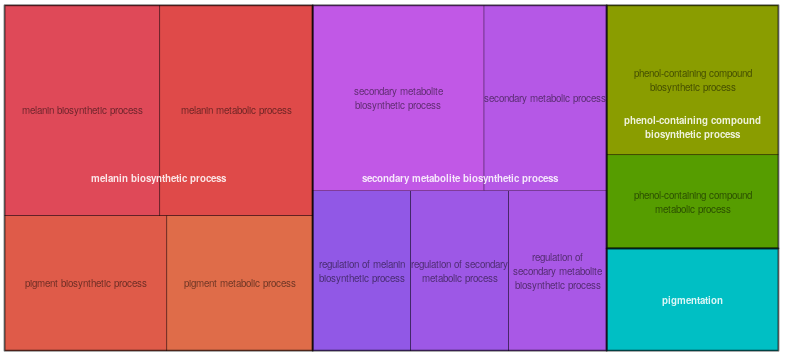
\includegraphics[width=1\textwidth]{img/chap2/chap2_revigo_resume_enrich_skin.png}
    \caption[Résumé des enrichissements sur GO par carte proportionnelle de l'intersection peau exposée au soleil, peau non exposée au soleil et muqueuse œsophagienne]{Résumé des enrichissements sur GO par carte proportionnelle de l'intersection peau exposée au soleil, peau non exposée au soleil et muqueuse œsophagienne. Chaque ensemble de GO terme partageant une ontologie parente commune (selon un score de similarité) est groupé sous une même couleur.}
    \label{figure:revigo_resume_melanine}
\end{figure}

La Figure \ref{figure:graphs_intersection_melanine} permet de constater que la relation TYR/SLC24A5 tend à augmenter avec l'âge dans la peau exposée ou non au soleil. Si l'augmentation est très marquée la peau non exposée au soleil, elle est bien moindre dans la peau non exposée. Ces résultats coïncident avec l'augmentation de la production de mélanine constatée chez la personne âgée pour compenser la diminution globale de la densité de mélanocytes \citeB{Gilchrest1979}. À l'inverse, la co-expression de CLEC12B avec SLC24A5 et TYR tend à diminuer avec l'âge, ainsi que l'intégralité de la co-expression de l'intersection.

La muqueuse œsophagienne elle semble interagir plus étroitement avec deux autres gènes, GML et ALX1 avec toutefois une interaction notable de la peau exposée au soleil avec ALX1 également. ALX1 est un gène jouant un rôle dans la migration cellulaire dans les structures craniofaciale lors du stade embryon, tandis que la fonction de GML est peu connu en dehors d'une potentielle contribution dans la voie d'activation de l'apoptose via p53 en cas de dommage à l'ADN. Comme visible en Figure \ref{figure:graphs_intersection_melanine}, la relation entre ces gènes ainsi qu'avec le gène TYR tend à diminuer dans la tranche âgée, qu'il s'agisse de la muqueuse œsophagienne comme de la peau exposée au soleil.




\section{Discussion}

\subsection{La susceptibilité des tissus aux variations liées au vieillissement}

Le vieillissement peut être vu comme une imbrication de multiples phénomènes qui découlent d'une dérégulation du fonctionnement physiologique ou d'une réponse à cette dérégulation. En prenant en compte le système dans sa quasi-intégralité, les réseaux de co-expression permettent d'acquérir de nouvelles connaissances au-delà d'acteurs transcriptomiques individuels connus. Les variations au cours du temps des relations de co-expression entre gènes sont alors les témoins d'autant de voies d'activations qui s'altèrent. Leur suivi et mise en contraste au travers de la co-expression différentielle sont donc à leur tour un moyen supplémentaire de comprendre le déroulé des altérations \citeB{Sharan2006, Southworth2009}. En comparant ces dernières entre de multiples tissus, il est possible d'en déduire des mécanismes communs au vieillissement, et à l'inverse ceux spécifiques. Dans cette étude, on s'est donc attachés à étudier ce vieillissement d'un point de vue multi-dimensionnel en comparant les réseaux issus de multiples tissus, et ce, entre deux tranches d'âge extrêmes. 

Si le vieillissement tend à perturber de nombreuses fonctions physiologiques, il semble cependant que peu de gènes soient impactés ou impactant dans ce processus. Ainsi, comme cela a pu être observé auparavant \citeB{Avelar2019}, une minorité de gènes varie significativement entre les deux conditions (modules NP) et une proportion légèrement plus grande varie modérément (modules MP) (Figure \ref{figure:upset_intersection_genes_tissu_unpres_modpres}). Ces gènes suffisent pourtant à représenter une large majorité des phénomènes connus du vieillissement : perte d'homéostasie, instabilité génomique, inflammation, dérivés réactifs de l'oxygène, etc. (Table \ref{table:intersection_aging_global_phenomenons} et Figure \ref{figure:revigo_resume_4_enrich}). Si leur répartition est inégale entre les tissus, ceux en portant le plus coïncident avec les tissus ayant un fort taux de renouvellement \citeB{Armanios2012, Barker2010, Leblond1956} (Table \ref{table:intersection_aging_global_phenomenons}) à l'exception dans notre cas de la thyroïde dont le renouvellement cellulaire minimal est de 8 ans \citeB{Coclet1989Dec}. Malgré une évidence des modifications que subit le système endocrinien avec le vieillissement, l'impact de celui-ci sur la thyroïde reste peu documenté hors pathologies graves \citeB{Faggiano2011Sep}. En effet, les altérations endocrines thyroïdiennes (hypo ou hyperthyroïdies) sont souvent associées à un vieillissement "naturel" de la personne \citeB{Cooper2004Dec}. Il est donc présomptueux ici de s'essayer à trouver une cause d'autant de marques du vieillissement sans plus d'information. Pourtant, les indices d'un rôle de la thyroïde sur la longévité s'accumulent ces dernières années \citeB{Garasto2017Jul,Arosio2020Sep}. Renforcer les connaissances sur les altérations de la fonction thyroïdienne chez la personne âgée semble donc une voie intéressante pour l'amélioration de la durée de vie chez l'homme.


\subsection{La variation de la réponse inflammatoire issue du vieillissement}

L'inflammation chronique de faible intensité est une caractéristique majeure du vieillissement qu'on nomme en anglais "\textit{inflammaging}" \citeB{Franceschi2014Jun,Minciullo2015} et dont la complexité limite encore les connaissances à son sujet \citeB{Franceschi2017}. Si l'inflammation est un mécanisme bénéfique dans la réponse aigüe et temporaire à un pathogène, elle se retrouve délétère dans le cas du vieillissement malgré une faible intensité car elle est persistante. Ce phénomène assumé comme étant un précurseur de plusieurs autres phénomènes du vieillissement \citeB{Lopez-Otin2013} s'est retrouvé ici plutôt exprimé dans le tissu adipeux, la peau non exposée au soleil, ainsi que la thyroïde. Les enrichissements fonctionnels sont venu préciser cette composante de l'inflammation comme une réponse à une réaction virale. En cause, de nombreux régulateurs d'interférons de type I significativement enrichis malgré leur absence de l'intersection. Ceci s'explique à contrario par la présence de nombreux gènes de réponse aux interférons, stimulés en temps normal par la présence d'ARN ou ADN viral.

Les interférons de type I (IFN-I) sont des cytokines regroupant tous les interférons à l'exception des IFN-\textgamma{} et dont les interférons majoritaires sont les IFN-\textalpha{} et IFN-\textbeta{}. Ces IFN-I ont pour rôle, dans la réponse inflammatoire normale, d'entraver à la fois la réplication du virus et les cellules hôtes infectées. Pour cela, un large panel de gènes de réponse aux interférons, dont ceux détectés ici, est induit avec différents objectifs : interférer avec le trafic intracellulaire des vésicules, limiter la stabilité et la traduction des ARNm viraux, et entraîner une apoptose de la cellule au besoin via la voie d'activation de la protéine p53\citeB{Frisch2020}. Cependant l'intervention de ce mécanisme antiviral dans le cadre du vieillissement est encore mal compris. Une hypothèse prometteuse est que des éléments transposables, plus particulièrement les LINE-1 (\textit{long interspersed nuclear elements}) se retrouvent non réprimés avec l'âge en raison d'une dégradation des acteurs de leur répression (ex : des petits ARN ou \textit{small RNA} (smRNA) en anglais) \citeB{Kreiling2017Jan, DeCecco2019Feb, Frisch2020}. Ces LINE-1 codent alors pour diverses transcriptases inverses et autres protéines de rétro-transposition qui vont déclencher la réponse anti-virale associée à une sénescence \citeB{QiujingYu2015May}. S'il est admis que cette réponse varie de la "normale" antivirale, il reste toutefois difficile de comprendre comment les gènes antiviraux se comportent dans ce cadre non-viral \citeB{Frisch2020} et la raison pour laquelle des marqueurs de la sénescence sont produits.

Dans le cadre de notre étude, on a constaté que le gène antiviral RSAD2 induit par les interférons officie comme gène pivot de co-expression. Dans le cas de la peau non exposée au soleil, il collabore également étroitement avec deux autres gènes antiviraux de la famille OAS : OAS2 et OASL. Les gènes OAS ont déjà été auparavant associés à une réponse de type IFN-I induite par la sénescence et plus particulièrement l'accumulation d'ADN dans la cellule \citeB{DeCecco2019Feb} qui est une composante délétère du vieillissement. Concernant RSAD2, aucun lien direct chez l'humain n'a été mis en avant à ce jour, seulement chez la souris \citeB{Ma2020Mar}. La protéine produite par RSAD2 est connue pour limiter la réplication de l'ADN viral ou de l'ARN double brin viral bien que le mécanisme par lequel elle opère n'est pas entièrement clair \citeB{Fitzgerald2011Jan}. En plus d'être un potentiel marqueur de cette accumulation d'ADN liée aux éléments transposables, RSAD2 pourrait donc être un potentiel gène candidat pour le développement de médicaments anti-âge.


\subsection{L'altération de la régulation des mélanocytes et de la mélanogénèse avec l'âge}

Au-delà des manifestations communes du vieillissement, chaque tissu est affecté de façon plus spécifique dans sa physiologie. L'altération avec l'âge de la mélanogénèse est un de ces changements qu'on retrouve en toute logique uniquement dans les tissus disposant de mélanocytes. La peau est l'organe en disposant du plus grand nombre et se retrouve ainsi d'autant plus affecté par cette altération avec l'âge. Dans notre intersection liée à la mélanogénèse, l'hyper-pigmentation connue dans le vieillissement \citeB{Hakozaki2016Sep} s'est retranscrite par l'augmentation de la co-expression entre TYR et SLC24A5, respectivement catalyseur et régulateurs de la production d'eumélanine \citeB{Cullinane2011Oct, Ginger2008}, dans la peau exposée ou non au soleil. L'augmentation nettement plus grande dans la peau non exposée au soleil était toutefois inattendue étant donné que l'hyper-pigmentation a plutôt été relevée dans les peaux exposées au soleil en raison de la stimulation de la mélanogénèse par les UV \citeB{Gilchrest1979}. 

En plus d'une co-expression entre TYR et SLC24A5, une forte co-expression de CLEC12B a été montrée dans les deux tissus de peau. Une investigation de ce gène a révélé que peu d'information est connue sur ses fonctions et son implication dans la mélanogénèse. Des résultats préliminaires conséquents ont toutefois montré sa capacité à recruter les phosphorylases SHP-1/SHP-2 via son domaine ITIM \citeB{Sormani2019}, enzymes notamment connues pour leur implication dans la pigmentation dans le syndrome LEOPARD \citeB{Motegi2015}. Ce nouveau gène impliqué dans la pigmentation de la peau coïncide ainsi avec les estimations d'un plus grand nombre de gènes contribuant au spectre de pigmentation que ceux actuellement connus et majeurs comme MC1R \citeB{Parra2004Nov}. 
Contrairement à la co-expression entre TYR et SLC24A5, CLEC12B tend à perdre sa synergie avec l'âge. Avec l'âge, CLEC12B tend à perdre sa synergie avec TYR et SLC24A5. L'inactivation de CLEC12B ayant démontré une diminution de la pigmentation dans un modèle de peau humaine reconstruite \citeB{Sormani2019}, on peut alors se demander si ce gène ne serait pas impliqué dans le phénomène de dépigmentation global de la peau lors du vieillissement (phénomène parallèle à l'hyper-pigmentation locale). Plus précisément, CLEC12B serait impliqué dans les voies d'inhibition de la prolifération des mélanocytaire par le biais de p53/p21/p27 \citeB{montaudie2019} et on pourrait envisager alors que la diminution de la densité de mélanocytes avec l'âge serait en partie dû à la diminution de co-expression de CLEC12B avec TYR et SLC24A5. Une validation expérimentale par une limitation partielle de l'expression de CLEC12B pourrait être à même de confirmer cette hypothèse.

La muqueuse œsophagienne et la peau étant toutes deux des tissus dotés d'un épithélium squameux stratifié dérivé de la crête neurale \citeB{delaPava1963}, il est cohérent de les retrouver au sein d'une même intersection. Pierson et al. ont d'ailleurs montré la proximité de leur expression dans leur étude du jeu de données GTEx \citeB{Pierson2015}. S'il est commun que la peau soit étudiée pour son contenu en mélanocytes, il est beaucoup moins courant que le contenu en mélanocytes de la muqueuse œsophagienne soit étudié. Le rôle de ce type cellulaire dans ce tissu reste ainsi encore mal compris en dehors des parallèles avec les mécanismes déjà connus dans la peau comme la réduction des dérivés réactifs de l'oxygène ou la fixation de certaines molécules organiques et ions métalliques \citeB{Tolleson2005}. 

Dans cette intersection côté muqueuse œsophagienne donc, la co-expression de TYR et SLC24A5 avec CLEC12B fait place à une co-expression croisée de TYR et SLC24A45A avec ALX1 et GML. 
GML est un homologue des protéines de membrane ancrées de type glycosyl-phosphatidylinositol (GPI), mais dont la fonction encore inconnue est suspectée d'être liée à l'apoptose et la régulation du cycle cellulaire \citeB{Furuhata1996Nov}. Il a été constaté que son expression tend à ralentir la progression des cellules cancéreuses de l'œsophage et à augmenter la sensibilité des cellules cancéreuses à certaines chimiothérapies \citeB{Catalano2001May}. 
De son côté, ALX1 est un facteur de transcription impliqué dans la régulation de gènes liés au développement embryonnaire et à la migration cellulaire \citeB{Dee2013Jan}. Il a été détecté comme sous exprimé chez des embryons de souris irradié entraînant un retard de pigmentation de l'épithélium rétinien. 
Pris ensemble, ces gènes pourraient donc être soupçonnés d'être à l'origine de la régulation de la prolifération des mélanocytes dans la muqueuse œsophagienne, bien qu'aucune direction de régulation ne puisse être extrapolée de nos réseaux de co-expression en tant que tel. En revanche, on peut avancer que si une telle régulation existe, elle est perturbée avec le vieillissement d'après la diminution notable de la co-expression entre TYR et SLC24A5 (donc contraire à l'évolution de la co-expression dans la peau) coïncidant avec la forte diminution de leur co-expression avec ALX1 et GML ainsi qu'entre eux deux. 
Ces altérations et les fonctions pour lesquelles codent ces gènes évoquent logiquement le développement de mélanomes qui sont parmi les pathologies associées au vieillissement et où les fonctions de régulation de la prolifération des mélanocytes par ALX1 et GML pourraient entrer en jeu. Toutefois, le mélanome œsophagien reste une pathologie rare, même si la fréquence des mélanomes œsophagiens d'origine métastatique est plus élevée que celle des mélanomes œsophagiens d'origine primitive. Il reste donc compliqué d'évaluer l'impact de la diminution de co-expression de ALX1 et GML ainsi que SLC24A5 et TYR dans le vieillissement de la muqueuse œsophagienne. Si des études sont menées ultérieurement sur ces gènes ou sur le contenu en mélanocytes de la muqueuse œsophagienne, elles pourront potentiellement donner de nouvelles perspectives à ces résultats.





\section{Conclusion}

Grâce à leur capacité d'étude à plus large échelle, les réseaux de co-expression sont un outil à privilégier pour l'exploration multi-tissus d'un phénomène aussi global et complexe que le vieillissement. Notre mise en évidence de groupes gènes impliqués dans les deux phénomènes du vieillissement sur lesquels on s'est concentrés est encourageant quant à l'utilisation de la co-expression différentielle et l'étude des motifs impliqués. Des tissus portant les mêmes gènes d'altérés peuvent ainsi être étudiées via la co-expression et permettre d'établir un lien direct entre les gènes et les marques du vieillissement. Des phénomènes communs comme spécifiques de différents tissus ont pu être mis en évidence. Des limitations restent toutefois présentes sur la nécessité pour se faire d'un grand nombre d'échantillons dans les tranches d'âge jeunes, ou en tout cas pas sur tout type de tissu. 
% De même, une validation de ces résultats via expérimentalement reste un passage obligatoire et coûteux, bien que moins coûteux qu'un criblage à haut débit sans pré-sélection.
De même, une validation de ces résultats via expérimentalement reste un passage obligatoire et coûteux. Notre profilage par co-expression différentielle aura toutefois permis de réduire leur coût financier en ciblant un sous ensemble de gènes à étudier par rapport à un criblage à haut débit sans pré-sélection.





% ##############################################################################

% Idées initiales de chapitre 2 - abandonnées :
% \begin{itemize}
%     \item Rajout d'information protéique pour "consolider" le réseau ?
%     \item Rajout d'une méthode de réseau consensus à GWENA ?
%     \item Differential co-expression avec un autre tissu sur lequel on peut avoir des jeux de données jeune/vieux pour récup les genes communs au vieillissement, ceux specifique à un tissu ou l'autres, et ceu combinant le vieillissement specifique au tissu ?
%     \item Une étude de l'impacte de la filtration sur l'état du réseau final ? Il n'y a rien de systemique dans la littérature, personne qui en fasse une review. Parsana et al. (alexis battle team) a fait ça en 2019 pour tester la PC-correction uniquement. Ils ont simulé des données scale free + des données scale free mimiquant GTEx et essayé de déterminer l'impact en calculant un FDR
% \end{itemize}


\bibliographystyleB{unsrt}
\bibliographyB{chap2-biblio}
% \bibliographystyleB{plain-fr}
% \bibliographyB{bibliographie}                         % chapitre 2, etc.
\chapter*{Conclusion}         % ne pas numéroter
\phantomsection\addcontentsline{toc}{chapter}{Conclusion} % dans TdM

Une thèse ou un mémoire devrait normalement se terminer par une
conclusion, placée avant les annexes, le cas échéant. Celle-ci est
traitée comme un chapitre normal, sauf qu'elle n'est pas numérotée.


% Publi utile pour les perspectives :
% https://onlinelibrary.wiley.com/doi/abs/10.1111/gbb.12106


Le vieillissement est un phénomène dont la complexité n'a d'égal que la multiplicité de ses manifestations. Tantôt origine, tantôt conséquence, les phénomènes de sa manifestations impactent de nombreux mécanismes cellulaire et moléculaires : sénescence et cellules souches, inflammation chronique de faible intensité, raccourcissement des télomères, etc. \cite{Lopez-Otin2013}. Pour distinguer de façon certaine chacun des altérations basales chez chaque individu, un nombre important d'échantillons est nécessaire. L'étude GTEx est à ce jour le plus gros regroupement de séquençage en terme d'individus/tissus non ciblé sur une pathologie. Sa réalisation permet d'étudier le vieillissement non plus dans ses manifestations les plus détaillées mais bien de rechercher les mécanismes communs à beaucoup des tissus composant le corps humain. Cependant                            % conclusion
\setcounter{chapter}{5}
\setcounter{section}{0}
\setcounter{figure}{0}   
\chapter*{Discussion}         % ne pas numéroter
\phantomsection\addcontentsline{toc}{chapter}{Discussion} % dans TdM

\section{L'apport de mes travaux sur l'étude du vieillissement}

\begin{itemize}
    \item La création d'un outil de type pipeline avec comparison et analyse intégrée
    \item La démonstration de son application chez le muscle et le ciblage de gènes potentiellements liés au vieillissement
    \item whatever secodn article
    \item Les études de quantification de l'expression c'est bien, mais grâce au RNA-seq on peut aller explorer d'autres pan du transcriptome et potentiellement faire des recoupements avec des phénomènes/mécanismes observés via quantification de l'expression
\end{itemize}

\section{limitations}
\begin{itemize}
    \item Les réseaux de co-expression comme moyen d'étude mais de nouvelles méthodes moins bruitée se mettent en place %% https://www.nature.com/articles/s42255-020-00304-4 et https://www.nature.com/articles/s42255-020-00295-2 (pas un article mais un News and Views qui resume)
    \item Ne permettent pas directement de connaitre le sens de régulation, il faut d'autres analyses pour inférer le sens de la relation dans un réseau de co-expression. Avec ça vient les soucis d'inférence évoqués par marie laure : co-regulation, manque de puissance stat..
\end{itemize}



\section{Perspectives}

- la potentielle application dans l'étude du cancer ou dans une étude comparative concernant la perte de connectivité observée là bas également 10.1371/journal.pone.0087075
- l'utilisation dans des populations d'ethinies plus minoritaires, malheureusement les données et bdd sont faibles par rapport à la puissance stat requise
- approches multi-omiques avec intégration de réseaux protein-protein % <- ptet plus dans mise en contexte des travaux                            % discussion

\renewcommand{\bibsection}{\chapter*{\bibname}}  % Repasse en chapitre la biblio qui était en section et enlève le numero devant
\phantomsection\addcontentsline{toc}{chapter}{Bibliographie} % rajoute la biblio dans la TdM 
\bibliographystyle{plain-fr}                    % bibliographie
\bibliography{bibliographie}                    % nom du fichier .bib

% \appendix                       % annexes le cas échéant
% \chapter*{Annexes}
% \addcontentsline{toc}{chapter}{Annexes}
% \chapter{Questions en bio-informatique}

Cette annexe a pour vocation de regrouper les nombreuses questions qui ont pu se poser durant cette thèse. Bien que parfois basiques, elles n'en sont pas moins légitimes. Beaucoup de ces questions on vu leur réponse plus longue que prévu à trouver en raison de consensus installés dans la communauté, de reflex de chercheur, etc. sans savoir l'origine de ceux-ci.

\section{Pourquoi normalisation log2 pour le microarray ?}
Le log pour passer à une échelle symétrique autour de 0, le 2 car c'est + facile à interpréter, chaque fois qu'on augmente le ratio Ti de 1, on double la up regulation 
%% (https://www.researchgate.net/post/Why_do_we_usually_use_Log2_when_normalizing_the_expression_of_genes et https://www.nature.com/articles/ng1032z)

      % annexe
% \chapter{NetRep statistics detail}


\todo{TODO : récupérer, résumer (et traduire ?) l'explication et l'interprétation biologique des 7 métriques disponibles dans les Supplemental Experimental Procedures de la publication de netrep (https://doi.org/10.1016/j.cels.2016.06.012)}

Source : Document S1. Supplemental Experimental Procedures, Figures S1–S7, and Tables S1–S4, S6, and S7 from 

% \chapter{Demande d'accès dbGaP aux données protégées de GTEx}

\label{annexe:dbgap}

\section{Query title}
Muscle gene co-expression in multiple age range for sarcopenia condition exploration

\section{Research use statement}
As a multi factorial phenomena, aging is a complex condition to study. Current analysis of transcriptomic data joined with phenotypic ones have unravel few genes and environmental variables impacting it. However, aging remains not fully understood. These may come from current approaches focusing on single factors while aging is more about interaction between many of them. This is why we would like to study it through the spectrum of the co-expression networks. However, because aging is already complex by itself, we will focus on a single tissue in the beginning : muscle. Reasons are myopenia and dynapenia (known together as sarcopenia) are responsible for loss of autonomy, weak metabolic aggression resistance, and increased mortality.
By using our yet to be published pipeline developed in our lab, we aim to build gene co-expression modules and network from transcriptomic data and characterize them with external resources. This pipeline begin with a quality assessment of the data, based on the technique used to get transcriptomic information (either microarray or RNA-Seq). It then compute co-expression levels and detects modules by using the WGCNA package. Additionnal steps are then performed to fully charachterize the modules : biological enrichment, topological study, phenotipic association, differentially expressed and condition-specific gene positionning.The external resources used to it include : enrichment databases (GO, KEGG, etc.), phenotypic information (exact age, condition of death, ethnicity), and age related databases (Digital aging atlas, Aging map, etc.). The use of these complementary information represents no additional risk to participants since only summarized gene information we'll be used in the form of modules. No other raw transcriptomics data will be combined to the GTEx data, but only a comparison of the modules built on each datasets in order to study the reproductibility of our modules, and the comparison with modules built on sarcopenia dedicated datasets.
Phenotipyc information is the main reason for our current demand regarding protected datasets because we think precise age and cause of death will impact the aging expression. 
No collaboration with other institution is planned.
Finnally, this methodological work will advance the understanding of the genetic bases of the aging processes occurring in the muscle.


\section{Non-technical summary}
Aging affect every one of us. It is defined as the progressive degradation of biological functions inside the body. In the muscle, this results in a decreasing in muscle density and strength called sarcopenia. They are responsible for mobility difficulties, therefore autonomy, and a deficit in body protection against aggression, sometimes leading to death. With this risks at stake, it is understandable that a better understanding of aging processes in muscle is important for public health. Few single genes linked to it have already been discovered, however we still don't fully understand the mechanisms occurring and how to limit them. Gene expression is a witness of the changes in the body mechanisms. By studying the expression of the genes and the coordination between this levels of expression, therefore patterns of expression, we aim to detect news genes involved in muscle aging. Do to so, we regroup the most coordinated genes in entities called module and try to unravel the biological interactions which link them. Because some of this genes are already involved into other biological interactions, we can have an insight on the regulations that take place in this case by extrapolating information. These, will lead to the discovery of new genes associated with sarcopenia.

\hfill \break
\textit{Réalisé le 30/09/2019}

\textcolor[RGB]{220,220,220}{\rule{\linewidth}{0.2pt}}

\section{Access update : Research Progress}
Current analysis of the GTEx data focused on the skeletal muscle samples as we are studying sarcopenia and other aging impact on muscle. The RNAseq data was then split in two opposite age range (young and old) to emphase and capture the differences in aging through our newly developped differential gene co-expression network pipeline GWENA (\url{https://www.bioconductor.org/packages/release/bioc/html/GWENA.html}). 
A first analysis solely on the modules (gene groups) detected by GWENA in the young condition. A selection of interesting modules for muscle activity was achieved through a combinaison of moduels phenotypic association and gene sets enrichment. Inside one promissing module, hub genes connected in the network to genes involved in muscle activity allowed the identification of genes with strong evidence of contribution to muscle developpemnt and growth.
A second analysis used the full potential of the differential co-expression analysis offered by GWENA to find specific co-expression modules to aging. Important topological variation lead us to focus on one module. Further investigation is currently underway to characterise the origin of the specificity and this variations. 

\hfill \break
\textit{Réalisé le 01/12/2020}


\renewcommand{\appendixpagename}{Annexes}
\renewcommand{\appendixtocname}{Annexes}
\appendixpage
\begin{appendices}
    \chapter{Fichier additionnel associé au chapitre \ref{chapter:gwena}}

\begin{center}
{\huge Additional file 1}\\
\hfill \break
{\large GWENA: gene co-expression networks analysis and extended modules characterization in a single Bioconductor package} \\ 
\hfill \break
\textit{Gwenaëlle G. Lemoine, Marie-Pier Scott-Boyer, Bathilde Ambroise, Olivier Périn, Arnaud Droit}
\end{center}


%% ++++++++++++++++++++++++++++++++++++++++++++++++++++++++++++++++++++++++++++++++++++
%% +                    Z summary & combination NetRep                                +
%% ++++++++++++++++++++++++++++++++++++++++++++++++++++++++++++++++++++++++++++++++++++
\section{Supplementary Material and Method}
\subsection{Z summary detail and combination with NetRep}
\label{supp:supp_z_summary_detail}

As NetRep uses a permutation test with the null hypothesis of the module being not preserved, it can only return if the module is preserved or not significant. To determine if a module is not preserved or moderately preserved, a Z summary statistic is computed using the topological metrics defined by Langfelder et al. \cite{Langfelder2011} and renamed by NetRep \cite{Ritchie2016} such as : \\

\[Z_{summary} = \frac{Z_{density} + Z_{connectivity}}{2}\] \\

With the NetRep notation :
\begin{align*}
    Z_{density} & = median(Z_{cor.density},Z_{avg.edge.wei},Z_{mod.coh},Z_{avg.node.contrib}) \\
    Z_{connectivity} & = median(Z_{concor.wei.deg},Z_{concor.nod.contrib},Z_{concor.cor})
\end{align*} 

Where : 
\begin{small}
    \begin{align*}
        cor.density & = \text{mean}(vect.Matrix(\text{sign}(r_{ij}^{[ref](q)}r{ij}^{[test](q)})))    & vect.Matrix(A) & = (a_{2,1},a_{3,1},...,a_{n,1},a_{n,n-1}) \\
        avg.edge.wei & = density^{[test](q)} = \text{mean}(vect.Mat(A^{[test](q)}))        & r_{ij}^{[ref]} & = \text{cor}(x_i^{[ref]}, x_j^{[ref]})\\
        mod.coh & = \text{mean}_{i\in Mq}((kME_i^{[test](q)})^2)        & r_{ij}^{[test]} & = \text{cor}(x_i^{[test]}, x_j^{[test]})\\
        avg.node.contrib & = \text{mean}_{i\in Mq}(\text{sign}(kME_i^{[ref](q)})kME_i^{[test](q)})  \\
        concor.wei.deg & = \text{cor}(kIM)^{[ref](q)}, kIM^{[test](q)}  \\
        concor.nod.contrib & = \text{cor}_{i\in Mq}(kME_i^{[ref](q)},kME_i^{[test](q)})  \\
        concor.cor & = \text{cor}(vect.Matrix(r^{[ref](q)}), vect.Matrix(r^{[test](q)}))  \\
    \end{align*}
\end{small}

This score returns :
\begin{itemize}
    \item \textbf{Preserved} if the $Z_{summary}$ is above 10
    \item \textbf{Moderately preserved} if the $Z_{summary}$ is between 2 and 10
    \item \textbf{Unpreserved} if the $Z_{summary}$ is below 2
\end{itemize} 

\hfill\break

The results from both NetRep permutation test and the $Z_{summary}$ are then combined in GWENA as shown in Figure \ref{fig:supp_fig_comparison_schema_conclusion} and return a final result on the module comparison.

\begin{figure}[h!]
    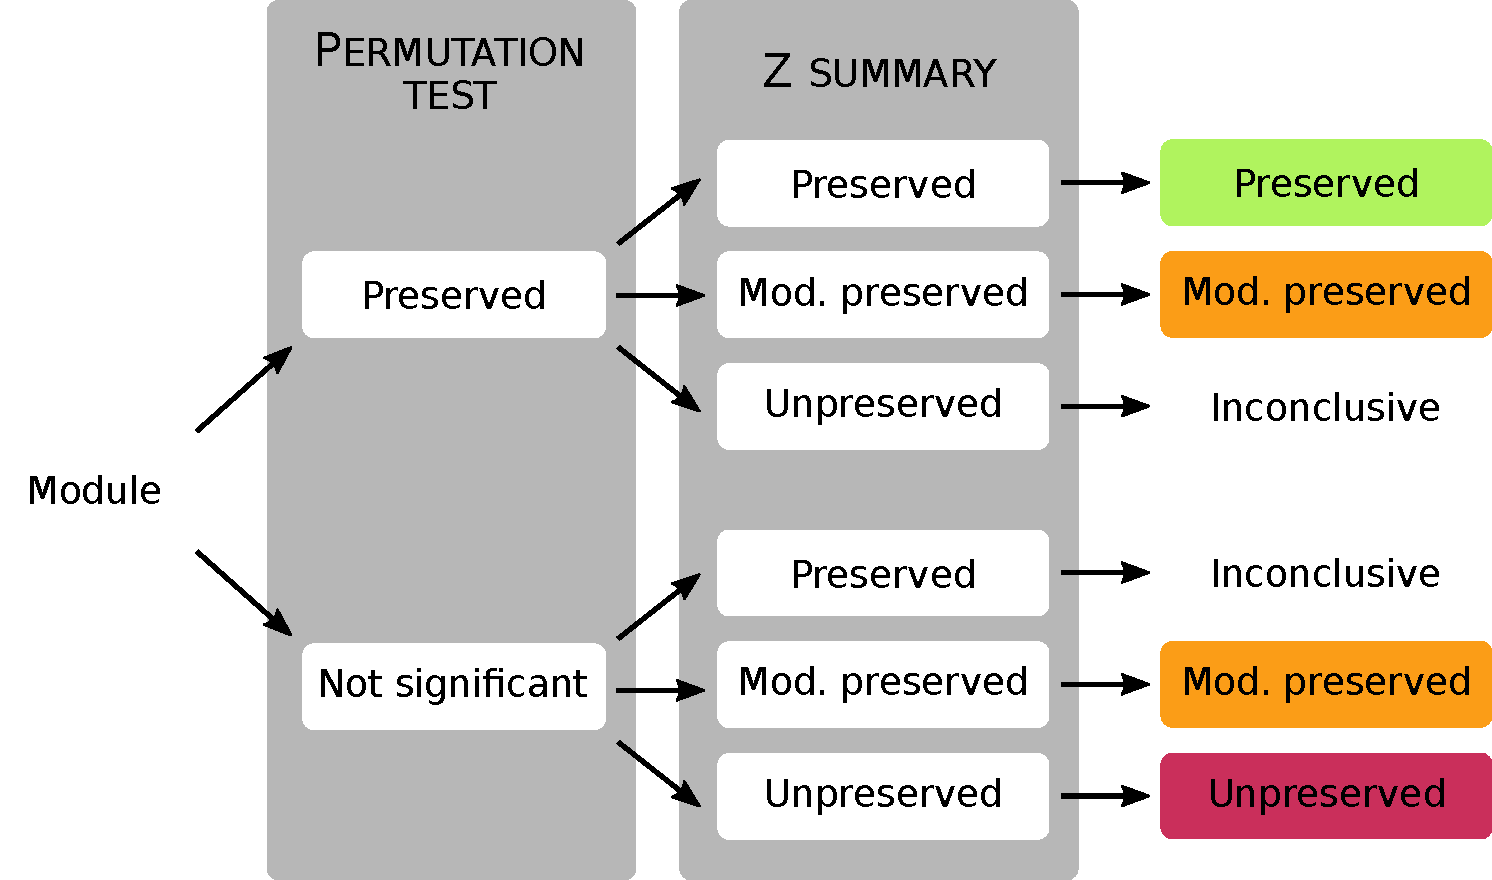
\includegraphics[width=\textwidth, center]{img/annexe_add_file_GWENA/additional_file_figure_1.pdf}
    \caption{Combination of the permutation test result ans the $Z_{summary}$ result in GWENA to return a final result on the module comparison.}
    \label{fig:supp_fig_comparison_schema_conclusion}
\end{figure}

%% ++++++++++++++++++++++++++++++++++++++++++++++++++++++++++++++++++++++++++++++++++++
%% +                                    Details data                                  +
%% ++++++++++++++++++++++++++++++++++++++++++++++++++++++++++++++++++++++++++++++++++++



\subsection{Details on case study data}
\label{supp:supp_detail_data_software}

Public data were obtained from GTEx v8 version on the GTEx Portal on 09/20/2020. 
Access to private data was subject to a request to dbGaP on accession number phs000424.v8.p2. Data were obtained on 10/21/2020.

\begin{table}[h!]
\begin{tabular}{ll}
\textbf{Data}      & \textbf{File}                                                     \\ \hline
Gene expression    & GTEx\_Analysis\_2017-06-05\_v8\_RNASeQCv1.1.9\_gene\_reads.gct.gz \\
Public annotation  & GTEx\_Analysis\_v8\_Annotations\_SampleAttributesDS.txt           \\
Private annotation & phs000424.v8.pht002742.v8.p2.c1.GTEx\_Subject\_Phenotypes.GRU.txt \\
Phenotype          & GTEx\_Analysis\_v8\_Annotations\_SubjectPhenotypesDS.txt         
\end{tabular}
\caption{Correspondence between file names and their contents}
% \label{}
\end{table}



%% ++++++++++++++++++++++++++++++++++++++++++++++++++++++++++++++++++++++++++++++++++++
%% +                                  PC-correction                                   +
%% ++++++++++++++++++++++++++++++++++++++++++++++++++++++++++++++++++++++++++++++++++++


\subsection{GTEx data normalization with PC-correction method}
\label{supp:supp_pc_correction}

In order to limit batch effect and handle the maximum of other co-founding effects, we chose to use a method based on PC-correction as recommended by Parsana et al. \cite{Parsana2019} for GTEx data. However age is usually included in this confounding factors, therefore is corrected. Since we're interested in gene changes we adapted the method to remove only the top $n$ PC correlated to age and which removed the least of genes correlating with age. The $n$ number of PC to remove was estimated by calculating the loss of correlation between phenotype and genes expression (Figure \ref{fig:supp_fig_ageing_correlation_density}) and confirmed by looking for the number of significantly correlated genes with two ageing gene databases (Figure \ref{fig:supp_fig_ageing_genes_overlapping}): GenAge \cite{Tacutu2018} and Digital Aging Atlas \cite{Craig2015}.

\begin{figure}[h!]
    % \centering
    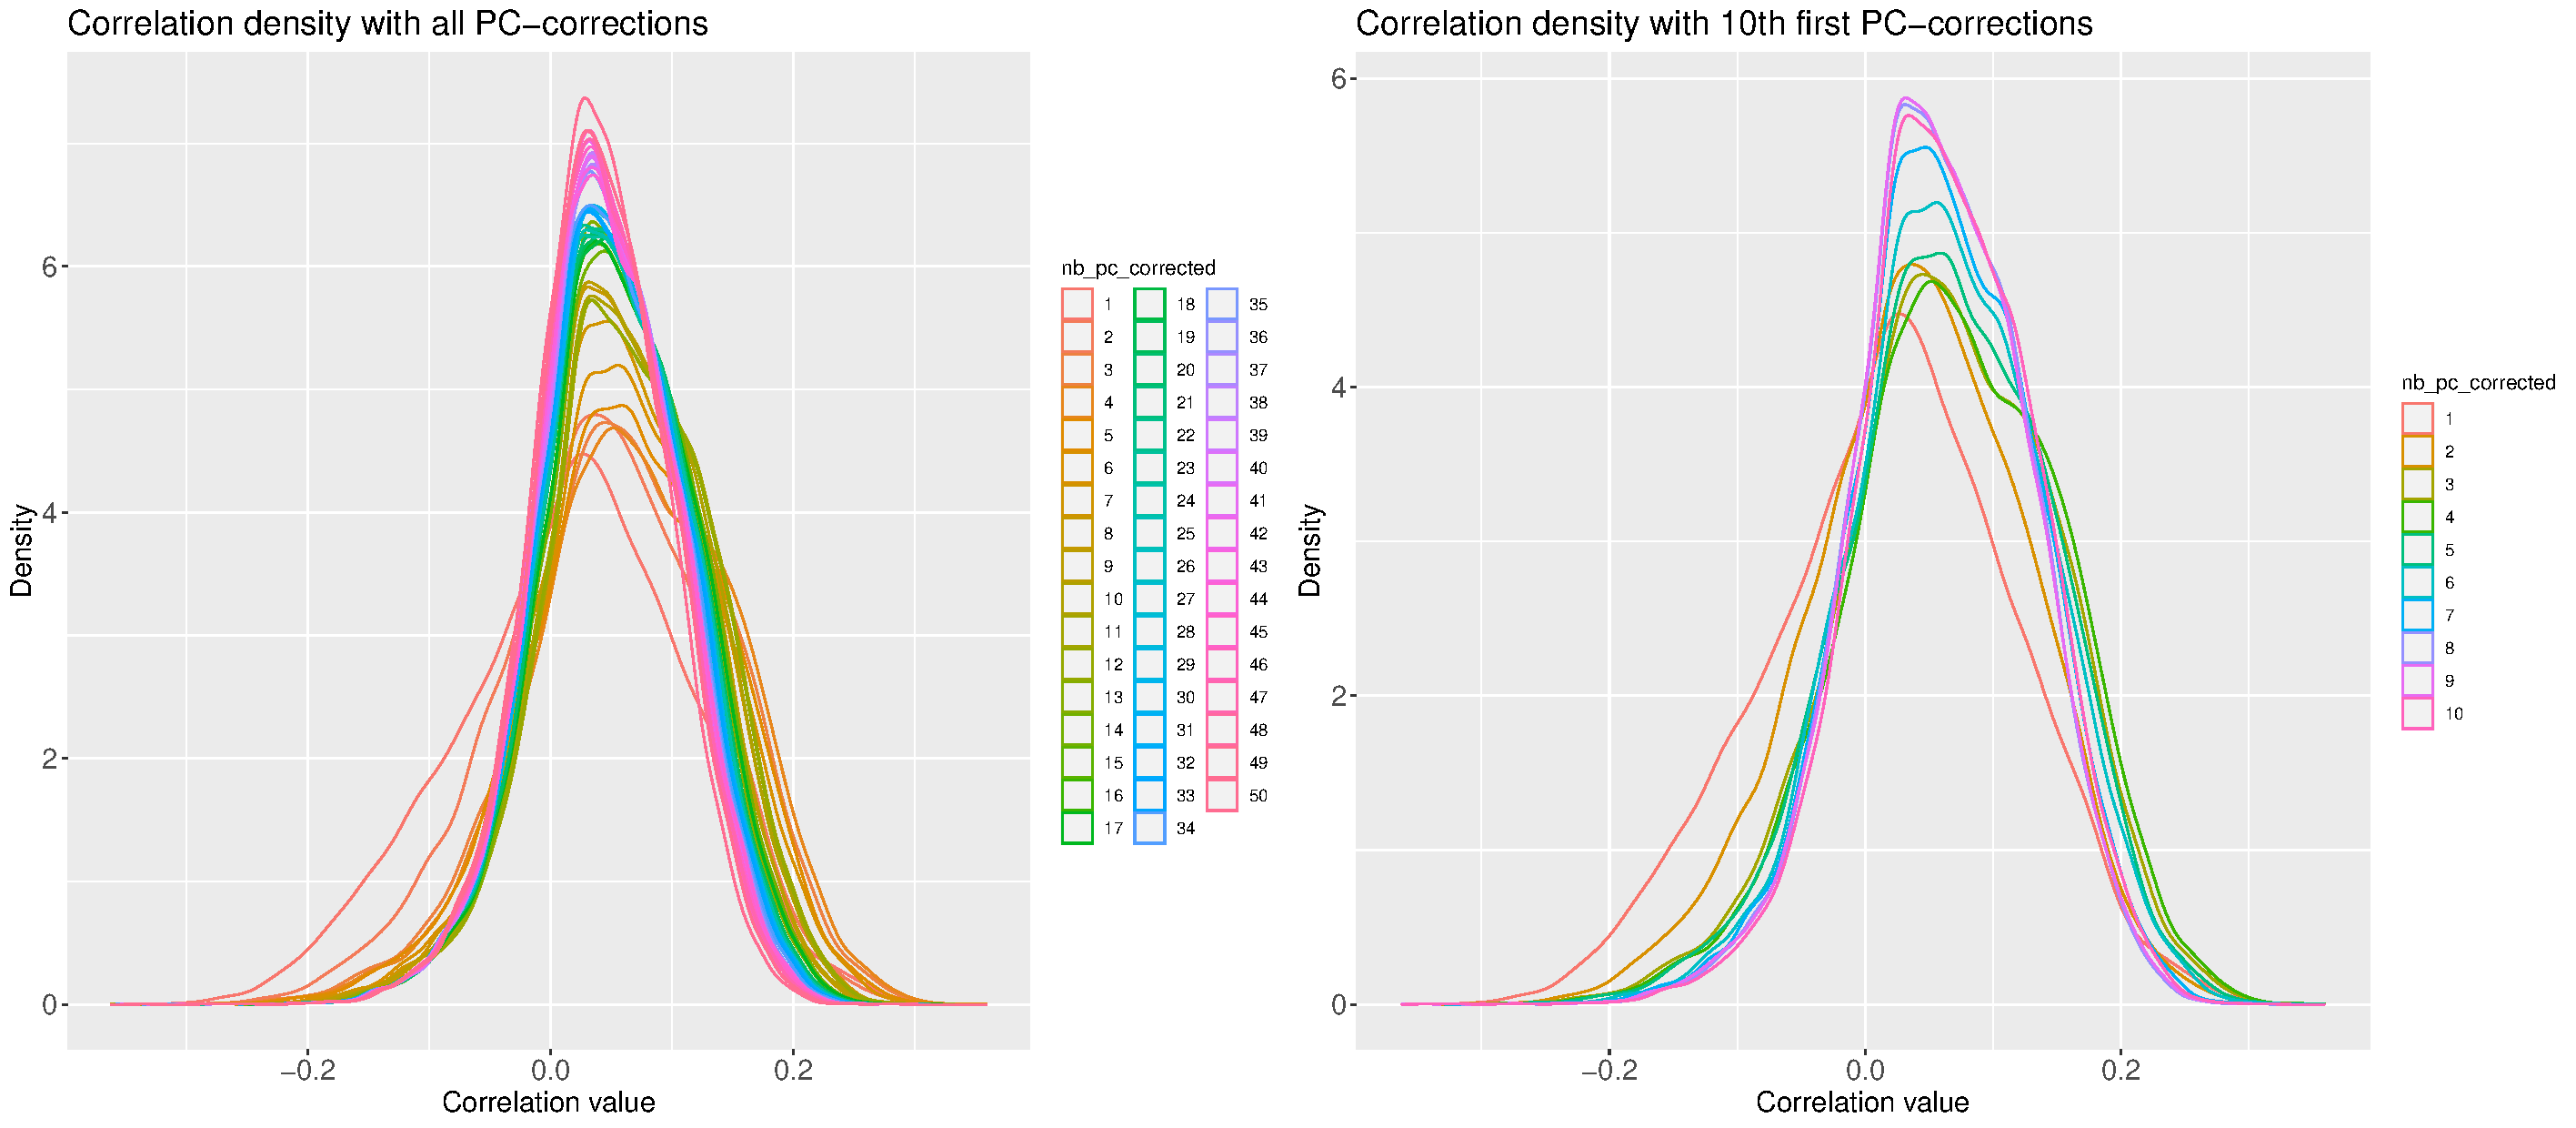
\includegraphics[width=\textwidth, center]{img/annexe_add_file_GWENA/additional_file_figure_2.pdf}
    \caption{Ageing genes correlation density with phenotype depending on the number of PC corrected. Left figure contains all PC correction tested. For clarity we filtered on the first 10 PC corrected on the right figure.}
    \label{fig:supp_fig_ageing_correlation_density}
\end{figure}

\begin{figure}[h!]
    % \centering
    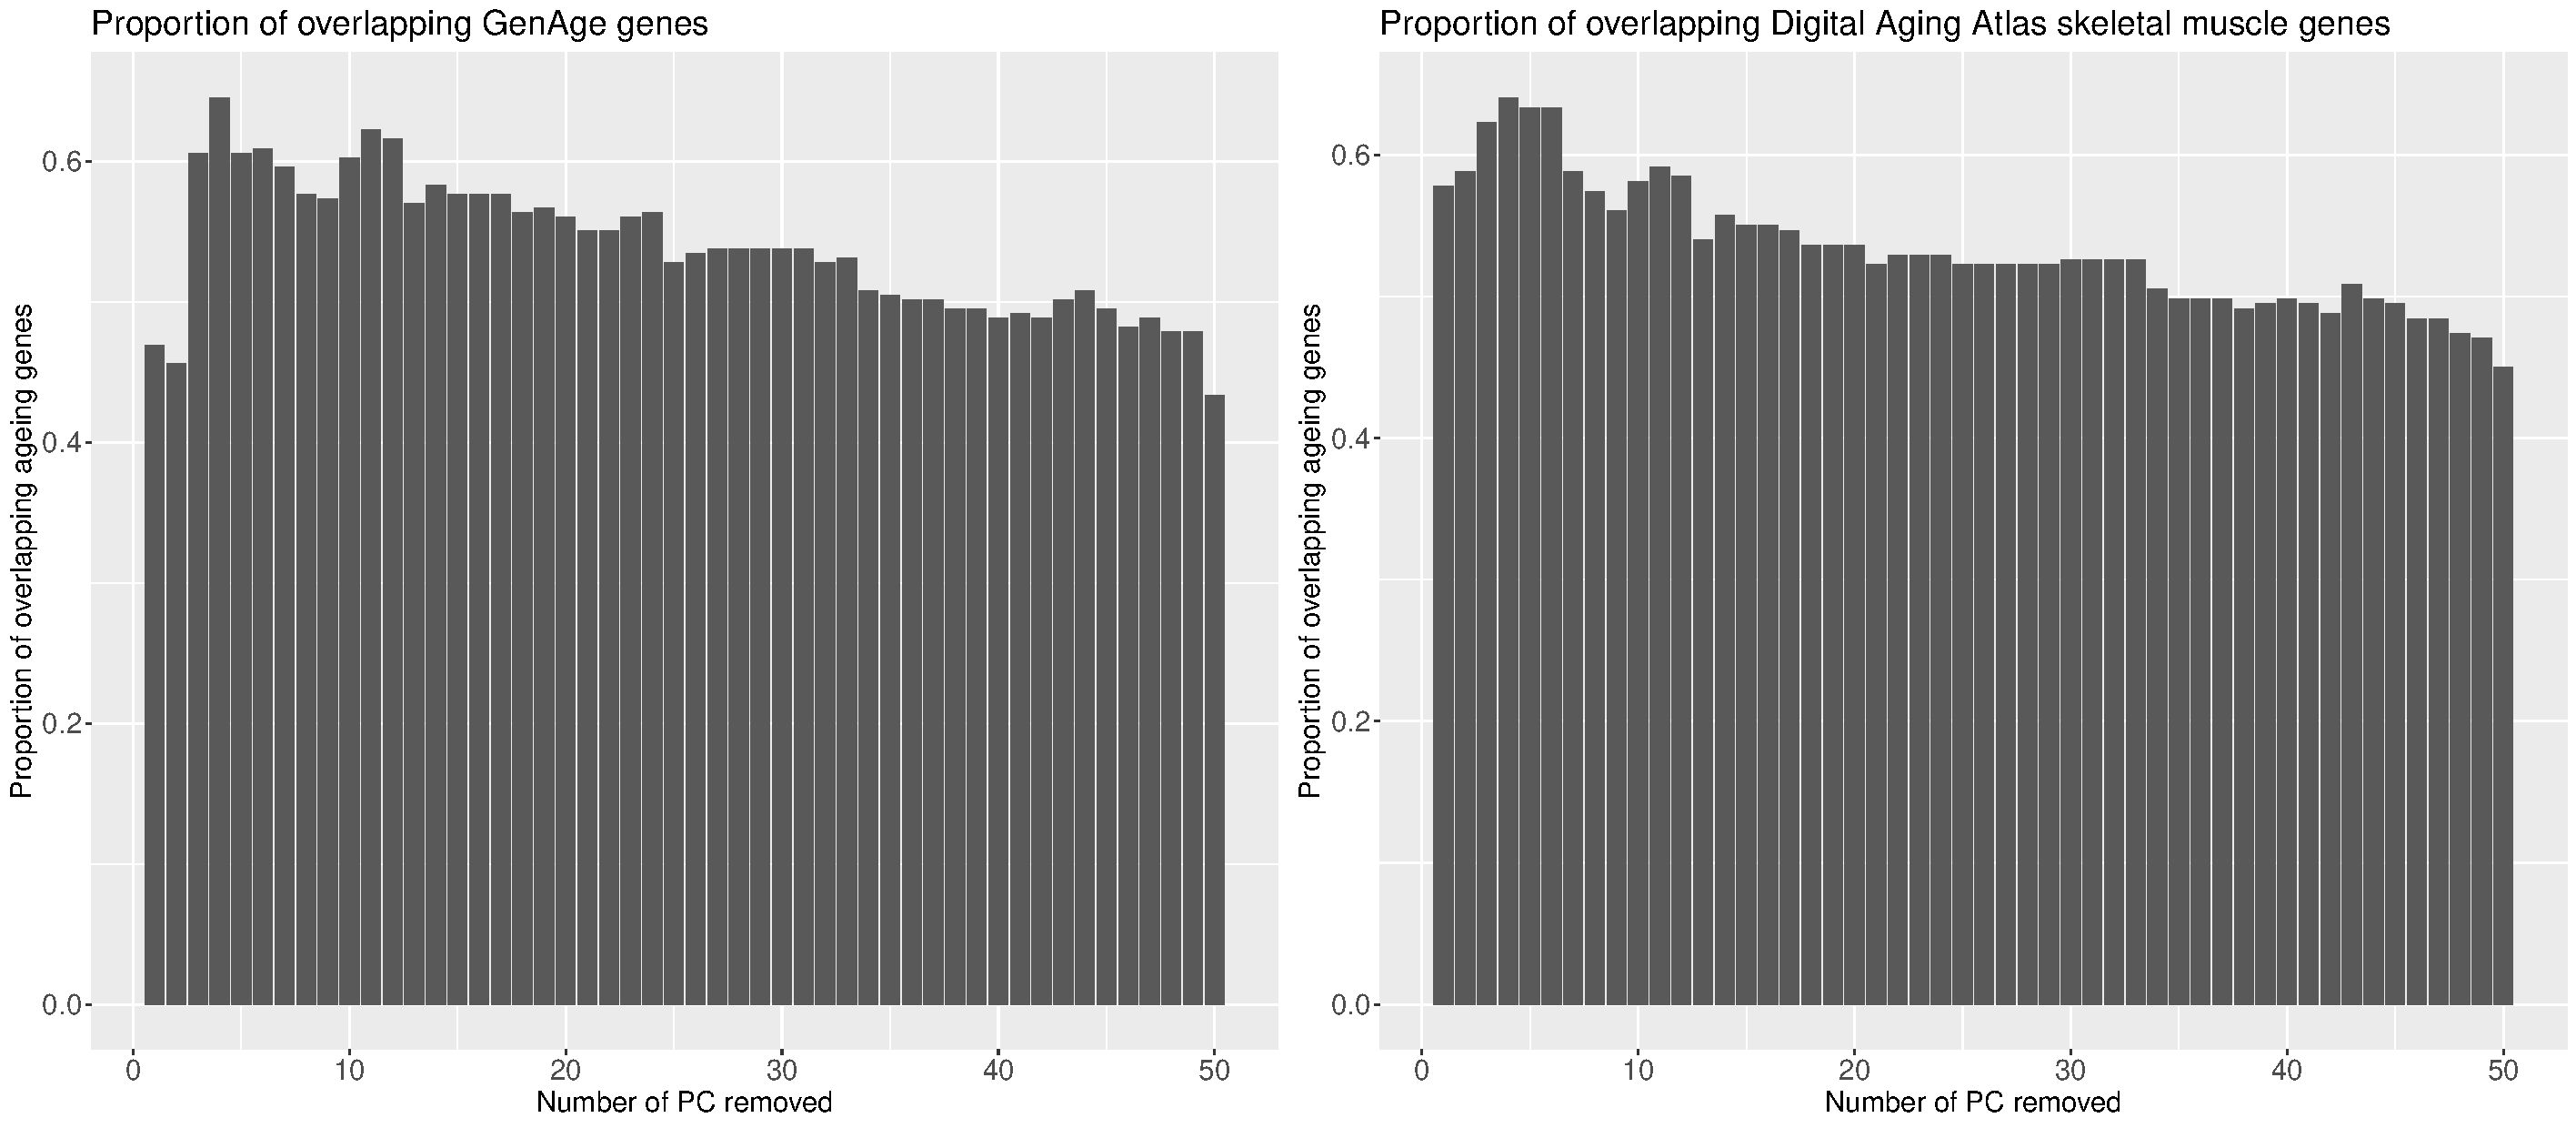
\includegraphics[width=\textwidth, center]{img/annexe_add_file_GWENA/additional_file_figure_3.pdf}
    \caption{Number of genes known to be associated with ageing.}
    \label{fig:supp_fig_ageing_genes_overlapping}
\end{figure}

Correlation density in Figure \ref{fig:supp_fig_ageing_correlation_density} suggest a similarity between the corrections from 2 to 5 PC removal. Combined with the proportion of overlapping known ageing genes in Figure \ref{fig:supp_fig_ageing_genes_overlapping} we determined the optimal number of PC $n$ to remove to be 4.

\clearpage
\section{Supplementary Results}
\subsection{Connectivity drop on all modules}
\label{supp:supp_connectivity_drop}

\begin{figure}[h!]
    \begin{adjustbox}{addcode=
        {\begin{minipage}{\width}}
        {
                \caption{Distribution of the connectivity for each gene by module between the two age range. Genes connectivity is ordered by increasing connectivity in the young condition (red).}
            \end{minipage}
        },rotate=90,center}
        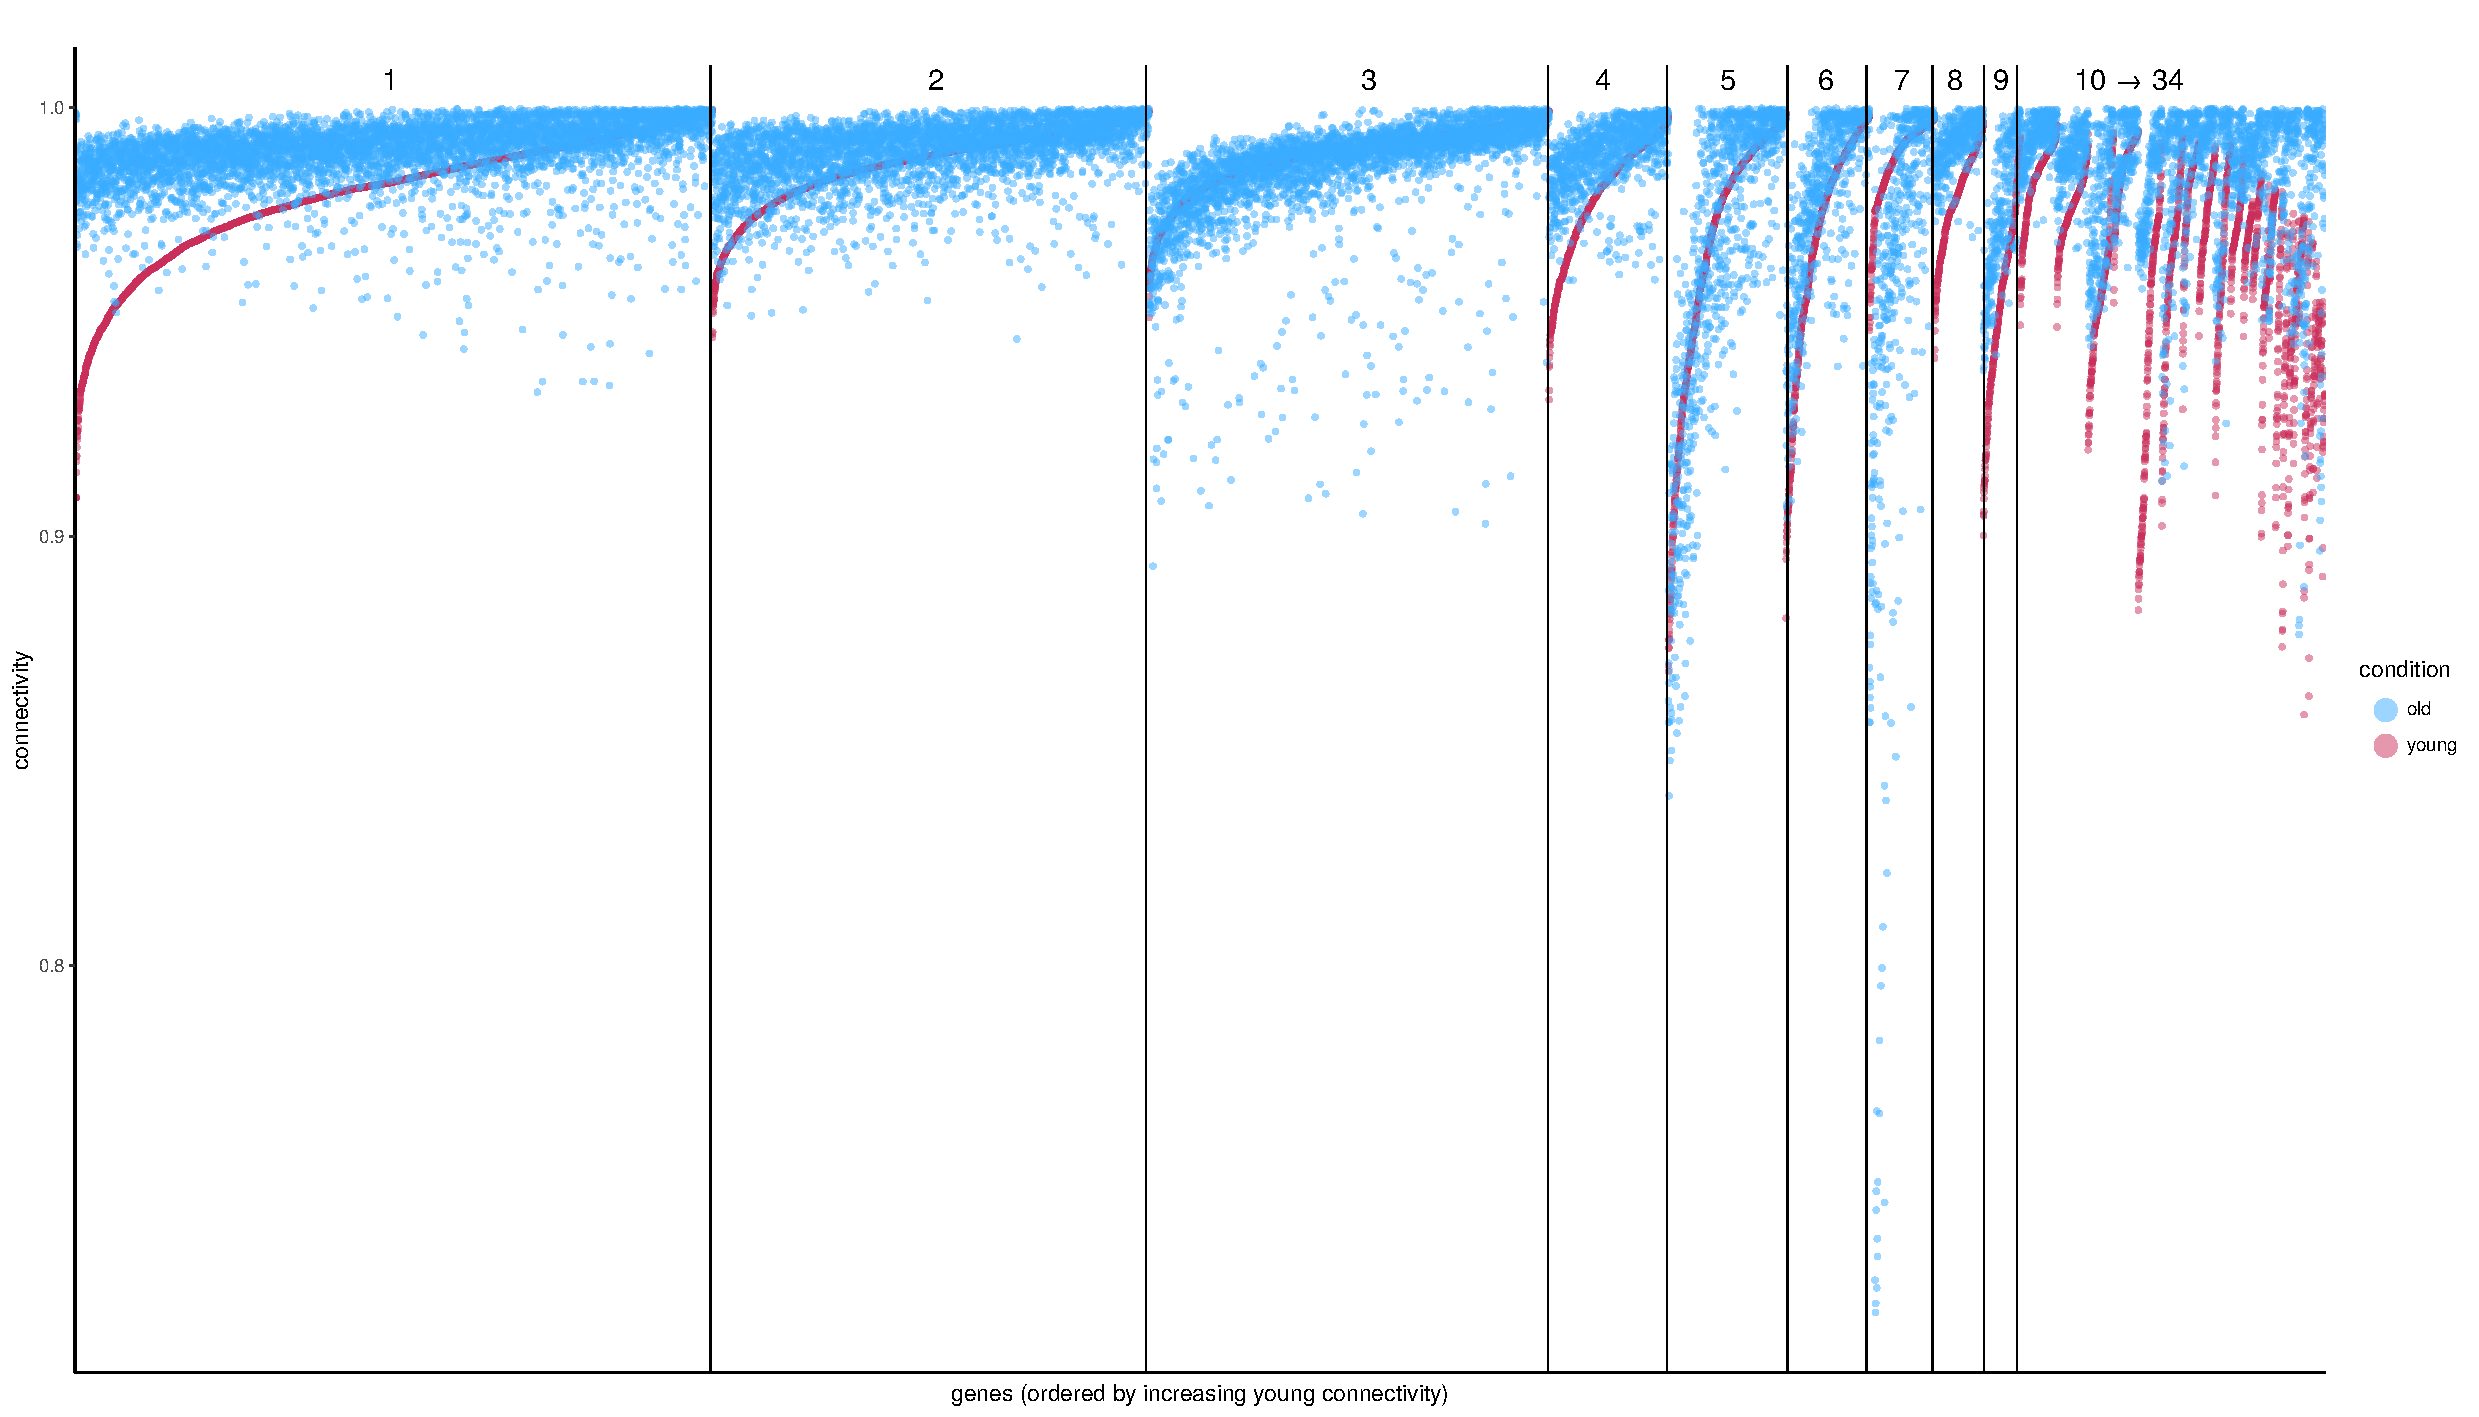
\includegraphics[scale=.476]{img/annexe_add_file_GWENA/additional_file_figure_4.pdf}%
    \end{adjustbox}
\end{figure}

\clearpage
\subsection{New enrichment terms in sub module 6 from module 7 old age range}
\label{supp:supp_sub_cluster_6_enrich_table}

% \resizebox{\textwidth}{!}{ % gneu gneu gneu marche pas
\LTcapwidth=\textwidth
% \setlength\LTright{3pt}
% \setlength\LTleft{0pt}
\begin{longtable}{@{}lp{5cm}lllp{5cm}l@{}}
\caption{Enrichment table from module 7 sub module 6 in old condition. Terms are sorted along their novelty (is the enrichment new compared to the enrichments from sub modules in the young age range) and then the source. Source is the enrichment database used on the gene set (GO:BP = Gene Ontology : Biological Process, GO:CC = Gene Ontology Cellular Compartment, GO:MF = Gene Ontology : Molecular Function, HP : Human Phenotype Ontology, WP = WikiPathway, KEGG = Kyoto Encyclopedia of Genes and Genomes, REAC = Reactome, TF = Transfac).}
\\ \hline
\textbf{source} & \textbf{term name}                                                                                                                & \textbf{is new} & \textbf{} & \textbf{source} & \textbf{term name}                                                                                                                                                    & \textbf{is new} \\ \hline
CORUM           & Fibrinogen complex                                                                                                                 & no               &           & GO:BP           & regulation of vasoconstriction                                                                                                                                         & yes              \\
GO:BP           & fibrinolysis                                                                                                                       & no               &           & GO:BP           & heterotypic cell-cell adhesion                                                                                                                                         & yes              \\
GO:BP           & negative regulation of blood coagulation                                                                                           & no               &           & GO:BP           & platelet aggregation                                                                                                                                                   & yes              \\
GO:BP           & negative regulation of hemostasis                                                                                                  & no               &           & GO:BP           & regulation of endothelial cell apoptotic process                                                                                                                       & yes              \\
GO:BP           & negative regulation of coagulation                                                                                                 & no               &           & GO:BP           & endothelial cell apoptotic process                                                                                                                                     & yes              \\
GO:BP           & negative regulation of wound healing                                                                                               & no               &           & GO:BP           & protein processing                                                                                                                                                     & yes              \\
GO:BP           & negative regulation of response to wounding                                                                                        & no               &           & GO:BP           & cell-matrix adhesion                                                                                                                                                   & yes              \\
GO:BP           & regulation of body fluid levels                                                                                                    & no               &           & GO:BP           & positive regulation of response to wounding                                                                                                                            & yes              \\
GO:CC           & blood microparticle                                                                                                                & no               &           & GO:BP           & positive regulation of blood circulation                                                                                                                               & yes              \\
GO:CC           & platelet alpha granule lumen                                                                                                       & no               &           & GO:BP           & vasoconstriction                                                                                                                                                       & yes              \\
GO:CC           & platelet alpha granule                                                                                                             & no               &           & GO:BP           & regulation of vesicle-mediated transport                                                                                                                               & yes              \\
GO:CC           & collagen-containing extracellular matrix                                                                                           & no               &           & GO:BP           & cell adhesion                                                                                                                                                          & yes              \\
GO:CC           & fibrinogen complex                                                                                                                 & no               &           & GO:BP           & biological adhesion                                                                                                                                                    & yes              \\
GO:CC           & extracellular space                                                                                                                & no               &           & GO:BP           & homotypic cell-cell adhesion                                                                                                                                           & yes              \\
GO:CC           & extracellular exosome                                                                                                              & no               &           & GO:BP           & vascular process in circulatory system                                                                                                                                 & yes              \\
GO:CC           & extracellular vesicle                                                                                                              & no               &           & GO:BP           & extrinsic apoptotic signaling pathway via death domain receptors                                                                                                       & yes              \\
GO:CC           & extracellular organelle                                                                                                            & no               &           & GO:CC           & secretory granule lumen                                                                                                                                                & yes              \\
GO:CC           & extracellular region                                                                                                               & no               &           & GO:CC           & cytoplasmic vesicle lumen                                                                                                                                              & yes              \\
GO:CC           & secretory granule                                                                                                                  & no               &           & GO:CC           & vesicle lumen                                                                                                                                                          & yes              \\
GO:CC           & secretory vesicle                                                                                                                  & no               &           & GO:CC           & extracellular matrix                                                                                                                                                   & yes              \\
GO:CC           & vesicle                                                                                                                            & no               &           & GO:CC           & cell surface                                                                                                                                                           & yes              \\
GO:MF           & enzyme inhibitor activity                                                                                                          & no               &           & GO:CC           & endoplasmic reticulum lumen                                                                                                                                            & yes              \\
HP              & Splenic rupture                                                                                                                    & no               &           & GO:CC           & cytoplasmic vesicle                                                                                                                                                    & yes              \\
WP              & COVID-19, thrombosis and anticoagulation                                                                                           & no               &           & GO:CC           & intracellular vesicle                                                                                                                                                  & yes              \\
GO:BP           & platelet degranulation                                                                                                             & yes              &           & GO:CC           & chylomicron                                                                                                                                                            & yes              \\
GO:BP           & regulation of blood coagulation                                                                                                    & yes              &           & GO:CC           & very-low-density lipoprotein particle                                                                                                                                  & yes              \\
GO:BP           & regulation of hemostasis                                                                                                           & yes              &           & GO:CC           & triglyceride-rich plasma lipoprotein particle                                                                                                                          & yes              \\
GO:BP           & regulation of coagulation                                                                                                          & yes              &           & GO:CC           & external side of plasma membrane                                                                                                                                       & yes              \\
GO:BP           & regulation of wound healing                                                                                                        & yes              &           & GO:CC           & high-density lipoprotein particle                                                                                                                                      & yes              \\
GO:BP           & plasminogen activation                                                                                                             & yes              &           & GO:CC           & plasma lipoprotein particle                                                                                                                                            & yes              \\
GO:BP           & regulation of response to wounding                                                                                                 & yes              &           & GO:CC           & lipoprotein particle                                                                                                                                                   & yes              \\
GO:BP           & protein activation cascade                                                                                                         & yes              &           & GO:CC           & protein-lipid complex                                                                                                                                                  & yes              \\
GO:BP           & blood coagulation, fibrin clot formation                                                                                           & yes              &           & GO:MF           & signaling receptor binding                                                                                                                                             & yes              \\
GO:BP           & vesicle-mediated transport                                                                                                         & yes              &           & GO:MF           & chaperone binding                                                                                                                                                      & yes              \\
GO:BP           & regulated exocytosis                                                                                                               & yes              &           & GO:MF           & immunoglobulin binding                                                                                                                                                 & yes              \\
GO:BP           & negative regulation of fibrinolysis                                                                                                & yes              &           & GO:MF           & lipoprotein particle receptor binding                                                                                                                                  & yes              \\
GO:BP           & exocytosis                                                                                                                         & yes              &           & GO:MF           & extracellular matrix structural constituent                                                                                                                            & yes              \\
GO:BP           & zymogen activation                                                                                                                 & yes              &           & HP              & Menometrorrhagia                                                                                                                                                       & yes              \\
GO:BP           & blood coagulation                                                                                                                  & yes              &           & HP              & Abnormality of the common coagulation pathway                                                                                                                          & yes              \\
GO:BP           & hemostasis                                                                                                                         & yes              &           & HP              & Spontaneous abortion                                                                                                                                                   & yes              \\
GO:BP           & coagulation                                                                                                                        & yes              &           & HP              & Abnormality of coagulation                                                                                                                                             & yes              \\
GO:BP           & regulation of fibrinolysis                                                                                                         & yes              &           & HP              & Hypofibrinogenemia                                                                                                                                                     & yes              \\
GO:BP           & positive regulation of heterotypic cell-cell adhesion                                                                              & yes              &           & HP              & Abnormality of circulating fibrinogen                                                                                                                                  & yes              \\
GO:BP           & regulation of cell-substrate adhesion                                                                                              & yes              &           & HP              & Joint swelling                                                                                                                                                         & yes              \\
GO:BP           & negative regulation of response to external stimulus                                                                               & yes              &           & HP              & Abnormality of the coagulation cascade                                                                                                                                 & yes              \\
GO:BP           & negative regulation of blood vessel diameter                                                                                       & yes              &           & HP              & Abnormal delivery                                                                                                                                                      & yes              \\
GO:BP           & negative regulation of response to stimulus                                                                                        & yes              &           & HP              & Abnormal thrombosis                                                                                                                                                    & yes              \\
GO:BP           & regulation of heterotypic cell-cell adhesion                                                                                       & yes              &           & KEGG            & Complement and coagulation cascades                                                                                                                                    & yes              \\
GO:BP           & positive regulation of blood coagulation                                                                                           & yes              &           & KEGG            & Platelet activation                                                                                                                                                    & yes              \\
GO:BP           & positive regulation of hemostasis                                                                                                  & yes              &           & KEGG            & Cholesterol metabolism                                                                                                                                                 & yes              \\
GO:BP           & positive regulation of coagulation                                                                                                 & yes              &           & MIRNA           & hsa-miR-409-3p                                                                                                                                                         & yes              \\
GO:BP           & wound healing                                                                                                                      & yes              &           & MIRNA           & hsa-miR-144-3p                                                                                                                                                         & yes              \\
GO:BP           & negative regulation of multicellular organismal process                                                                            & yes              &           & REAC            & Platelet degranulation                                                                                                                                                 & yes              \\
GO:BP           & positive regulation of cell-substrate adhesion                                                                                     & yes              &           & REAC            & Response to elevated platelet cytosolic Ca2+                                                                                                                           & yes              \\
GO:BP           & secretion by cell                                                                                                                  & yes              &           & REAC            & Platelet activation, signaling and aggregation                                                                                                                         & yes              \\
GO:BP           & negative regulation of endothelial cell apoptotic process                                                                          & yes              &           & REAC            & Regulation of Insulin-like Growth Factor (IGF) transport and uptake by Insulin-like Growth Factor Binding Proteins (IGFBPs) & yes              \\
GO:BP           & positive regulation of vasoconstriction                                                                                            & yes              &           & REAC            & Post-translational protein phosphorylation                                                                                                                             & yes              \\
GO:BP           & export from cell                                                                                                                   & yes              &           & REAC            & Hemostasis                                                                                                                                                             & yes              \\
GO:BP           & negative regulation of cellular process                                                                                            & yes              &           & REAC            & GRB2:SOS provides linkage to MAPK signaling for Integrins                                                                                                              & yes              \\
GO:BP           & regulation of response to stress                                                                                                   & yes              &           & REAC            & p130Cas linkage to MAPK signaling for integrins                                                                                                                        & yes              \\
GO:BP           & positive regulation of substrate adhesion-dependent cell spreading                      & yes              &           & REAC            & Regulation of TLR by endogenous ligand                                                                                                                                 & yes              \\
GO:BP           & regulation of blood vessel diameter                                                                                                & yes              &           & REAC            & Common Pathway of Fibrin Clot Formation                                                                                                                                & yes              \\
GO:BP           & regulation of tube diameter                                                                                                        & yes              &           & REAC            & Integrin signaling                                                                                                                                                     & yes              \\
GO:BP           & negative regulation of extrinsic apoptotic signaling pathway via death domain receptors & yes              &           & REAC            & Signaling by high-kinase activity BRAF mutants                                                                                                                         & yes              \\
GO:BP           & regulation of tube size                                                                                                            & yes              &           & REAC            & Platelet Aggregation (Plug Formation)                                                                                                                                  & yes              \\
GO:BP           & cell-substrate adhesion                                                                                                            & yes              &           & REAC            & Formation of Fibrin Clot (Clotting Cascade)                                                                                                                            & yes              \\
GO:BP           & post-translational protein modification                                                                                            & yes              &           & REAC            & MAP2K and MAPK activation                                                                                                                                              & yes              \\
GO:BP           & response to wounding                                                                                                               & yes              &           & REAC            & Signaling by moderate kinase activity BRAF mutants                                                                                                                     & yes              \\
GO:BP           & secretion                                                                                                                          & yes              &           & REAC            & Signaling downstream of RAS mutants                                                                                                                                    & yes              \\
GO:BP           & regulation of response to external stimulus                                                                                        & yes              &           & REAC            & Paradoxical activation of RAF signaling by kinase inactive BRAF                                                                                                        & yes              \\
GO:BP           & platelet activation                                                                                                                & yes              &           & REAC            & Signaling by RAS mutants                                                                                                                                               & yes              \\
GO:BP           & transport                                                                                                                          & yes              &           & REAC            & Signaling by BRAF and RAF fusions                                                                                                                                      & yes              \\
GO:BP           & response to stress                                                                                                                 & yes              &           & REAC            & Oncogenic MAPK signaling                                                                                                                                               & yes              \\
GO:BP           & establishment of localization                                                                                                      & yes              &           & REAC            & Dissolution of Fibrin Clot                                                                                                                                             & yes              \\
GO:BP           & negative regulation of epithelial cell apoptotic process                                                                           & yes              &           & REAC            & Integrin cell surface interactions                                                                                                                                     & yes              \\
GO:BP           & regulation of cell adhesion                                                                                                        & yes              &           & TF              & Factor: HNF1A; motif: GGTTAATNATTAMC                                                                                                                                   & yes              \\
GO:BP           & regulation of substrate adhesion-dependent cell spreading                                                                          & yes              &           & TF              & Factor: HNF-1alpha; motif: GGTTAATNWTTAMCN                                                                                                                             & yes              \\
GO:BP           & induction of bacterial agglutination                                                                                               & yes              &           & TF              & Factor: Sox-2; motif: NNNNNAACAAWGN; match class: 1                                                                                                                    & yes              \\
GO:BP           & regulation of response to stimulus                                                                                                 & yes              &           & WP              & Folate Metabolism                                                                                                                                                      & yes              \\
GO:BP           & proteolysis                                                                                                                        & yes              &           & WP              & Selenium Micronutrient Network                                                                                                                                         & yes              \\
GO:BP           & negative regulation of biological process                                                                                          & yes              &           & WP              & Human Complement System                                                                                                                                                & yes              \\
GO:BP           & regulation of cell-cell adhesion                                                                                                   & yes              &           & WP              & Blood Clotting Cascade                                                                                                                                                 & yes              \\
GO:BP           & regulation of extrinsic apoptotic signaling pathway via death domain receptors          & yes              &           & WP              & Fibrin Complement Receptor 3 Signaling Pathway                                                                                                                         & yes              \\
GO:BP           & positive regulation of wound healing                                                                                               & yes              &           & WP              & Vitamin B12 Metabolism                                                                                                                                                 & yes             

\label{supp:table_c6_enrich}
\end{longtable}


The distribution of the newly and previously found terms in the enrichment analysis across the the sub-modules from young and old age range (Figure \ref{fig:supp_fig_upset_subclusters_enrichments}).

\begin{figure}[h!]
    % \centering
    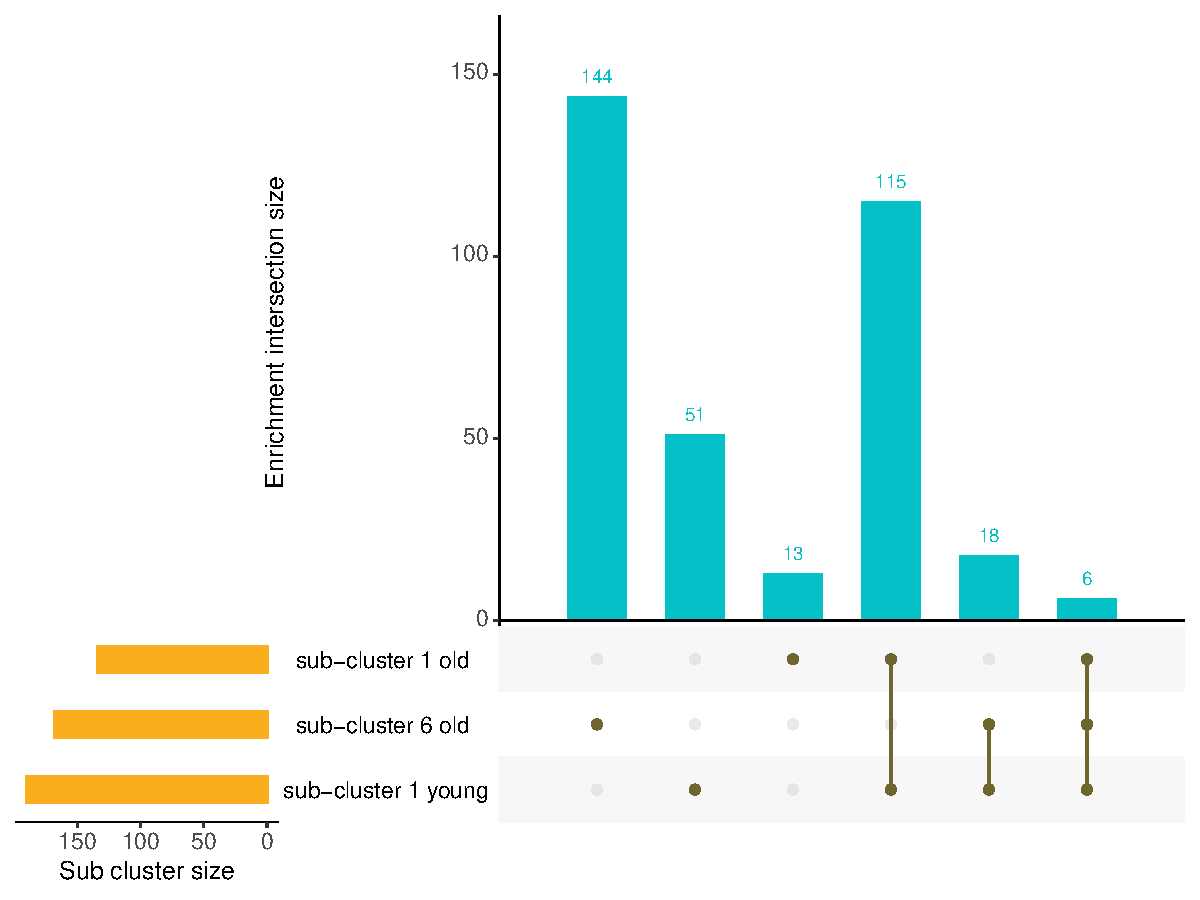
\includegraphics[width=\textwidth, center]{img/annexe_add_file_GWENA/additional_file_figure_5.pdf}
    \caption{Overlap between the enrichments found in sub-cluster 1 young, sub-cluster 1 old, and sub-cluster 6 old.(Upset diagram)}
    \label{fig:supp_fig_upset_subclusters_enrichments}
\end{figure} 


% \hfill \break
% \clearpage
% \bibliographystyle{unsrt}
% \bibliography{additional_file_1}
    \chapter{Demande d'accès dbGaP aux données protégées de GTEx}

\label{annexe:dbgap}

\section{Query title}
Muscle gene co-expression in multiple age range for sarcopenia condition exploration

\section{Research use statement}
As a multi factorial phenomena, aging is a complex condition to study. Current analysis of transcriptomic data joined with phenotypic ones have unravel few genes and environmental variables impacting it. However, aging remains not fully understood. These may come from current approaches focusing on single factors while aging is more about interaction between many of them. This is why we would like to study it through the spectrum of the co-expression networks. However, because aging is already complex by itself, we will focus on a single tissue in the beginning : muscle. Reasons are myopenia and dynapenia (known together as sarcopenia) are responsible for loss of autonomy, weak metabolic aggression resistance, and increased mortality.
By using our yet to be published pipeline developed in our lab, we aim to build gene co-expression modules and network from transcriptomic data and characterize them with external resources. This pipeline begin with a quality assessment of the data, based on the technique used to get transcriptomic information (either microarray or RNA-Seq). It then compute co-expression levels and detects modules by using the WGCNA package. Additionnal steps are then performed to fully charachterize the modules : biological enrichment, topological study, phenotipic association, differentially expressed and condition-specific gene positionning.The external resources used to it include : enrichment databases (GO, KEGG, etc.), phenotypic information (exact age, condition of death, ethnicity), and age related databases (Digital aging atlas, Aging map, etc.). The use of these complementary information represents no additional risk to participants since only summarized gene information we'll be used in the form of modules. No other raw transcriptomics data will be combined to the GTEx data, but only a comparison of the modules built on each datasets in order to study the reproductibility of our modules, and the comparison with modules built on sarcopenia dedicated datasets.
Phenotipyc information is the main reason for our current demand regarding protected datasets because we think precise age and cause of death will impact the aging expression. 
No collaboration with other institution is planned.
Finnally, this methodological work will advance the understanding of the genetic bases of the aging processes occurring in the muscle.


\section{Non-technical summary}
Aging affect every one of us. It is defined as the progressive degradation of biological functions inside the body. In the muscle, this results in a decreasing in muscle density and strength called sarcopenia. They are responsible for mobility difficulties, therefore autonomy, and a deficit in body protection against aggression, sometimes leading to death. With this risks at stake, it is understandable that a better understanding of aging processes in muscle is important for public health. Few single genes linked to it have already been discovered, however we still don't fully understand the mechanisms occurring and how to limit them. Gene expression is a witness of the changes in the body mechanisms. By studying the expression of the genes and the coordination between this levels of expression, therefore patterns of expression, we aim to detect news genes involved in muscle aging. Do to so, we regroup the most coordinated genes in entities called module and try to unravel the biological interactions which link them. Because some of this genes are already involved into other biological interactions, we can have an insight on the regulations that take place in this case by extrapolating information. These, will lead to the discovery of new genes associated with sarcopenia.

\hfill \break
\textit{Réalisé le 30/09/2019}

\textcolor[RGB]{220,220,220}{\rule{\linewidth}{0.2pt}}

\section{Access update : Research Progress}
Current analysis of the GTEx data focused on the skeletal muscle samples as we are studying sarcopenia and other aging impact on muscle. The RNAseq data was then split in two opposite age range (young and old) to emphase and capture the differences in aging through our newly developped differential gene co-expression network pipeline GWENA (\url{https://www.bioconductor.org/packages/release/bioc/html/GWENA.html}). 
A first analysis solely on the modules (gene groups) detected by GWENA in the young condition. A selection of interesting modules for muscle activity was achieved through a combinaison of moduels phenotypic association and gene sets enrichment. Inside one promissing module, hub genes connected in the network to genes involved in muscle activity allowed the identification of genes with strong evidence of contribution to muscle developpemnt and growth.
A second analysis used the full potential of the differential co-expression analysis offered by GWENA to find specific co-expression modules to aging. Important topological variation lead us to focus on one module. Further investigation is currently underway to characterise the origin of the specificity and this variations. 

\hfill \break
\textit{Réalisé le 01/12/2020}

    \chapter{Enrichissements des intersections de gènes en chapitre 2}
\label{annexe:chap_2_genes_intersect_enrichments}

Résultats des tests d'enrichissement effectués grâce à GWENA sur les intersections ayant au moins 3 tissus et 5 gènes lors du chapitre \ref{chapter:multidim}. Pour rappel :
\begin{itemize}
    \item{\textbf{GO} : Gene Ontology}
    \item{\textbf{GO:MF} : GO Molecular Function}
    \item{\textbf{GO:BP} : GO Biological Process}
    \item{\textbf{GO:CC} : GO Cellular Compartment}
    \item{\textbf{KEGG} : Kyoto Encyclopedia of Genes and Genomes}
    \item{\textbf{REAC} : Reactome}
    \item{\textbf{WP} : WikiPathway}
    \item{\textbf{TF} : TRANSFAC}
    \item{\textbf{MIRNA} : mirTarBase}
    \item{\textbf{HPA} : Human Protein Atlas}
    \item{\textbf{CORUM} : Comprehensive Resource of Mammalian protein complexes}
    \item{\textbf{HP} : Human Phenotype Ontology}
\end{itemize}


\section*{esophagus\_muscularis\_mod\_pres \newline skin\_sun\_exposed\_mod\_pres \newline thyroid\_mod\_pres}

\begin{longtable}{ll}
\toprule
Source & Nom du terme enrichit\\
\midrule
CORUM & Cell-cell junction complex (ARHGAP10-CTNNA1)\\
GO:BP & dicarboxylic acid catabolic process\\
HP & Hypoglutaminemia\\
HP & Abnormal CSF glutamine family amino acid concentration\\
HP & Abnormal CSF glutamine concentration\\
HP & Decreased CSF glutamine concentration\\
\bottomrule
\end{longtable}

\section*{esophagus\_muscularis\_mod\_pres \newline nerve\_tibial\_mod\_pres \newline skin\_sun\_exposed\_mod\_pres}

\begin{longtable}{ll}
\toprule
Source & Nom du terme enrichit\\
\midrule
CORUM & Seipin-lipin1 complex\\
GO:BP & adenosine to inosine editing\\
GO:BP & base conversion or substitution editing\\
GO:MF & phenylethanolamine N-methyltransferase activity\\
GO:MF & creatine:sodium symporter activity\\
GO:MF & XTP binding\\
GO:MF & ITP binding\\
\bottomrule
\end{longtable}

\section*{esophagus\_muscularis\_mod\_pres \newline nerve\_tibial\_mod\_pres \newline skin\_sun\_exposed\_mod\_pres \newline thyroid\_mod\_pres}

\begin{longtable}{ll}
\toprule
Source & Nom du terme enrichit\\
\midrule
GO:MF & dGTPase activity\\
GO:MF & triphosphoric monoester hydrolase activity\\
GO:MF & guanyl deoxyribonucleotide binding\\
GO:MF & dGTP binding\\
HPA & skin 1; melanocytes[High]\\
HPA & testis; peritubular cells[High]\\
\bottomrule
\end{longtable}

\section*{esophagus\_mucosa\_mod\_pres \newline skin\_not\_sun\_exposed\_mod\_pres \newline skin\_sun\_exposed\_mod\_pres}

\begin{longtable}{ll}
\toprule
Source & Nom du terme enrichit\\
\midrule
GO:BP & melanin biosynthetic process\\
GO:BP & melanin metabolic process\\
GO:BP & secondary metabolite biosynthetic process\\
GO:BP & phenol-containing compound biosynthetic process\\
GO:BP & secondary metabolic process\\
GO:BP & pigment biosynthetic process\\
GO:BP & pigment metabolic process\\
GO:BP & pigmentation\\
GO:BP & phenol-containing compound metabolic process\\
GO:BP & regulation of secondary metabolic process\\
GO:BP & regulation of melanin biosynthetic process\\
GO:BP & regulation of secondary metabolite biosynthetic process\\
GO:MF & melanin-concentrating hormone receptor activity\\
HPA & retina; pigment epithelial cells[High]\\
\bottomrule
\end{longtable}

\section*{esophagus\_mucosa\_mod\_pres \newline muscle\_skeletal\_mod\_pres \newline thyroid\_mod\_pres}

\begin{longtable}{ll}
\toprule
Source & Nom du terme enrichit\\
\midrule
GO:BP & oxygen transport\\
GO:BP & gas transport\\
GO:BP & hydrogen peroxide catabolic process\\
GO:CC & hemoglobin complex\\
GO:CC & haptoglobin-hemoglobin complex\\
GO:MF & hemoglobin binding\\
GO:MF & haptoglobin binding\\
GO:MF & oxygen carrier activity\\
GO:MF & oxygen binding\\
GO:MF & peroxidase activity\\
GO:MF & oxidoreductase activity, acting on peroxide as acceptor\\
GO:MF & molecular carrier activity\\
\bottomrule
\end{longtable}

\section*{esophagus\_mucosa\_mod\_pres \newline muscle\_skeletal\_mod\_pres \newline skin\_sun\_exposed\_mod\_pres}

\begin{longtable}{ll}
\toprule
Source & Nom du terme enrichit\\
\midrule
GO:BP & response to nicotine\\
GO:MF & V1B vasopressin receptor binding\\
REAC & ADORA2B mediated anti-inflammatory cytokines production\\
\bottomrule
\end{longtable}

\section*{esophagus\_mucosa\_mod\_pres \newline muscle\_skeletal\_unpres \newline skin\_sun\_exposed\_mod\_pres}

\begin{longtable}{ll}
\toprule
Source & Nom du terme enrichit\\
\midrule
HP & Gonadal tissue inappropriate for external genitalia or chromosomal sex\\
\bottomrule
\end{longtable}

\section*{artery\_tibial\_mod\_pres \newline skin\_not\_sun\_exposed\_mod\_pres \newline skin\_sun\_exposed\_mod\_pres}

\begin{longtable}{ll}
\toprule
Source & Nom du terme enrichit\\
\midrule
GO:MF & neuropeptide receptor activity\\
\bottomrule
\end{longtable}

\section*{artery\_tibial\_mod\_pres \newline esophagus\_muscularis\_mod\_pres \newline thyroid\_mod\_pres}

\begin{longtable}{ll}
\toprule
Source & Nom du terme enrichit\\
\midrule
GO:BP & response to corticotropin-releasing hormone\\
GO:BP & cellular response to corticotropin-releasing hormone stimulus\\
GO:BP & regulation of type B pancreatic cell proliferation\\
GO:BP & type B pancreatic cell proliferation\\
GO:CC & transcription regulator complex\\
GO:CC & chromatin\\
GO:MF & DNA-binding transcription activator activity, RNA polymerase II-specific\\
GO:MF & DNA-binding transcription activator activity\\
GO:MF & glucocorticoid receptor binding\\
GO:MF & nuclear receptor activity\\
GO:MF & ligand-activated transcription factor activity\\
GO:MF & DNA-binding transcription factor activity, RNA polymerase II-specific\\
GO:MF & DNA-binding transcription factor activity\\
GO:MF & steroid hormone receptor binding\\
TF & Factor: ATF; motif: CNSTGACGTNNNYC; match class: 1\\
\bottomrule
\end{longtable}

\section*{artery\_tibial\_mod\_pres \newline esophagus\_mucosa\_mod\_pres \newline thyroid\_mod\_pres}
No enrichment found

\section*{artery\_tibial\_mod\_pres \newline esophagus\_mucosa\_mod\_pres \newline skin\_sun\_exposed\_mod\_pres}

\begin{longtable}{ll}
\toprule
Source & Nom du terme enrichit\\
\midrule
GO:BP & positive regulation of gastrulation\\
GO:BP & primitive streak formation\\
GO:BP & regulation of gastrulation\\
KEGG & Viral protein interaction with cytokine and cytokine receptor\\
\bottomrule
\end{longtable}

\section*{artery\_tibial\_mod\_pres \newline esophagus\_mucosa\_mod\_pres \newline skin\_sun\_exposed\_unpres}
No enrichment found

\section*{artery\_tibial\_mod\_pres \newline esophagus\_mucosa\_mod\_pres \newline nerve\_tibial\_mod\_pres}

\begin{longtable}{ll}
\toprule
Source & Nom du terme enrichit\\
\midrule
GO:CC & blood microparticle\\
GO:CC & platelet alpha granule lumen\\
GO:CC & platelet alpha granule\\
GO:CC & collagen-containing extracellular matrix\\
GO:CC & extracellular matrix\\
GO:CC & external encapsulating structure\\
KEGG & Complement and coagulation cascades\\
REAC & Platelet degranulation\\
REAC & Response to elevated platelet cytosolic Ca2+\\
TF & Factor: C/EBP; motif: NTTRCNNAANNN\\
WP & Complement and Coagulation Cascades\\
\bottomrule
\end{longtable}

\section*{artery\_tibial\_mod\_pres \newline esophagus\_mucosa\_mod\_pres \newline nerve\_tibial\_mod\_pres \newline thyroid\_mod\_pres}

\begin{longtable}{ll}
\toprule
Source & Nom du terme enrichit\\
\midrule
CORUM & Fibrinogen complex\\
GO:BP & negative regulation of wound healing\\
GO:BP & plasminogen activation\\
GO:BP & negative regulation of response to wounding\\
GO:BP & fibrinolysis\\
GO:BP & blood coagulation, fibrin clot formation\\
GO:BP & protein activation cascade\\
GO:BP & platelet degranulation\\
GO:BP & regulation of wound healing\\
GO:BP & negative regulation of blood coagulation\\
GO:BP & regulation of response to wounding\\
GO:BP & negative regulation of hemostasis\\
GO:BP & negative regulation of coagulation\\
GO:BP & zymogen activation\\
GO:BP & regulation of blood coagulation\\
GO:BP & regulation of hemostasis\\
GO:BP & regulation of coagulation\\
GO:BP & positive regulation of heterotypic cell-cell adhesion\\
GO:BP & regulation of heterotypic cell-cell adhesion\\
GO:BP & negative regulation of response to external stimulus\\
GO:BP & positive regulation of vasoconstriction\\
GO:BP & negative regulation of endothelial cell apoptotic process\\
GO:BP & negative regulation of extrinsic apoptotic signaling pathway via death domain receptors\\
GO:BP & positive regulation of substrate adhesion-dependent cell spreading\\
GO:BP & wound healing\\
GO:BP & negative regulation of epithelial cell apoptotic process\\
GO:BP & negative regulation of multicellular organismal process\\
GO:BP & induction of bacterial agglutination\\
GO:BP & regulation of substrate adhesion-dependent cell spreading\\
GO:BP & regulation of extrinsic apoptotic signaling pathway via death domain receptors\\
GO:BP & protein processing\\
GO:BP & heterotypic cell-cell adhesion\\
GO:BP & regulation of endothelial cell apoptotic process\\
GO:BP & platelet aggregation\\
GO:BP & regulation of vasoconstriction\\
GO:BP & endothelial cell apoptotic process\\
GO:BP & response to wounding\\
GO:BP & positive regulation of cell morphogenesis involved in differentiation\\
GO:BP & extrinsic apoptotic signaling pathway via death domain receptors\\
GO:BP & vasoconstriction\\
GO:BP & protein maturation\\
GO:BP & homotypic cell-cell adhesion\\
GO:BP & positive regulation of exocytosis\\
GO:BP & regulated exocytosis\\
GO:BP & regulation of cell morphogenesis involved in differentiation\\
GO:BP & blood coagulation\\
GO:BP & hemostasis\\
GO:BP & coagulation\\
GO:BP & positive regulation of peptide hormone secretion\\
GO:BP & regulation of epithelial cell apoptotic process\\
GO:BP & negative regulation of extrinsic apoptotic signaling pathway\\
GO:BP & substrate adhesion-dependent cell spreading\\
GO:BP & exocytosis\\
GO:BP & positive regulation of cell-substrate adhesion\\
GO:BP & epithelial cell apoptotic process\\
GO:BP & positive regulation of hormone secretion\\
GO:BP & blood vessel diameter maintenance\\
GO:BP & regulation of tube diameter\\
GO:BP & regulation of tube size\\
GO:BP & positive regulation of protein secretion\\
GO:BP & response to calcium ion\\
GO:BP & regulation of response to external stimulus\\
GO:BP & positive regulation of peptide secretion\\
GO:BP & regulation of extrinsic apoptotic signaling pathway\\
GO:BP & platelet activation\\
GO:BP & toll-like receptor signaling pathway\\
GO:BP & regulation of body fluid levels\\
GO:CC & blood microparticle\\
GO:CC & fibrinogen complex\\
GO:CC & collagen-containing extracellular matrix\\
GO:CC & platelet alpha granule lumen\\
GO:CC & extracellular matrix\\
GO:CC & external encapsulating structure\\
GO:CC & platelet alpha granule\\
GO:CC & secretory granule lumen\\
GO:CC & cytoplasmic vesicle lumen\\
GO:CC & vesicle lumen\\
GO:CC & extracellular exosome\\
GO:CC & extracellular vesicle\\
GO:CC & extracellular organelle\\
GO:CC & secretory granule\\
GO:CC & secretory vesicle\\
GO:CC & extracellular space\\
GO:CC & vesicle\\
GO:CC & extracellular region\\
GO:CC & cell surface\\
GO:MF & extracellular matrix structural constituent\\
HP & Splenic rupture\\
HP & Menometrorrhagia\\
HP & Spontaneous abortion\\
HP & Abnormality of circulating fibrinogen\\
HP & Hypofibrinogenemia\\
HP & Joint swelling\\
HP & Abnormality of the common coagulation pathway\\
HP & Gingival bleeding\\
HP & Cerebral hemorrhage\\
HP & Abnormality of the cerebral vasculature\\
HP & Abnormal delivery\\
HP & Venous thrombosis\\
HP & Epistaxis\\
HP & Abnormality of the coagulation cascade\\
KEGG & Complement and coagulation cascades\\
KEGG & Platelet activation\\
KEGG & Neutrophil extracellular trap formation\\
KEGG & Coronavirus disease - COVID-19\\
MIRNA & hsa-miR-409-3p\\
MIRNA & hsa-miR-144-3p\\
MIRNA & hsa-miR-29c-3p\\
MIRNA & hsa-miR-29b-3p\\
MIRNA & hsa-miR-29a-3p\\
REAC & Platelet degranulation\\
REAC & Response to elevated platelet cytosolic Ca2+\\
REAC & GRB2:SOS provides linkage to MAPK signaling for Integrins\\
REAC & p130Cas linkage to MAPK signaling for integrins\\
REAC & Regulation of TLR by endogenous ligand\\
REAC & Common Pathway of Fibrin Clot Formation\\
REAC & Platelet activation, signaling and aggregation\\
REAC & Integrin signaling\\
REAC & Signaling by high-kinase activity BRAF mutants\\
REAC & Platelet Aggregation (Plug Formation)\\
REAC & Formation of Fibrin Clot (Clotting Cascade)\\
REAC & MAP2K and MAPK activation\\
REAC & Signaling by RAF1 mutants\\
REAC & Signaling by RAS mutants\\
REAC & Paradoxical activation of RAF signaling by kinase inactive BRAF\\
REAC & Signaling by moderate kinase activity BRAF mutants\\
REAC & Signaling downstream of RAS mutants\\
REAC & Signaling by BRAF and RAF fusions\\
REAC & Oncogenic MAPK signaling\\
REAC & Integrin cell surface interactions\\
REAC & Hemostasis\\
REAC & Toll-like Receptor Cascades\\
TF & Factor: HNF1B; motif: NRTTAATNATTAACN\\
TF & Factor: HNF1A; motif: GGTTAATNATTAMC\\
WP & COVID-19, thrombosis and anticoagulation\\
WP & Blood Clotting Cascade\\
WP & Human Complement System\\
WP & Fibrin Complement Receptor 3 Signaling Pathway\\
WP & Folate Metabolism\\
WP & Selenium Micronutrient Network\\
\bottomrule
\end{longtable}

\section*{artery\_tibial\_mod\_pres \newline esophagus\_mucosa\_mod\_pres \newline muscle\_skeletal\_mod\_pres}
No enrichment found

\section*{artery\_tibial\_mod\_pres \newline esophagus\_mucosa\_mod\_pres \newline muscle\_skeletal\_mod\_pres \newline thyroid\_mod\_pres}

\begin{longtable}{ll}
\toprule
Source & Nom du terme enrichit\\
\midrule
GO:MF & IgA receptor activity\\
HP & Hypochromic microcytic anemia\\
HP & Abnormality of iron homeostasis\\
HP & Iron deficiency anemia\\
HP & Abnormal blood transition element cation concentration\\
HP & Microcytic anemia\\
HP & Hypochromic anemia\\
\bottomrule
\end{longtable}

\section*{artery\_tibial\_mod\_pres \newline esophagus\_mucosa\_mod\_pres \newline muscle\_skeletal\_unpres}

\begin{longtable}{ll}
\toprule
Source & Nom du terme enrichit\\
\midrule
CORUM & TCL1 homotrimer complex\\
GO:BP & cell wall disruption in other organism\\
GO:CC & high-density lipoprotein particle\\
GO:CC & plasma lipoprotein particle\\
GO:CC & lipoprotein particle\\
GO:CC & protein-lipid complex\\
GO:CC & zymogen granule\\
GO:MF & oligosaccharide binding\\
GO:MF & peptidoglycan binding\\
GO:MF & glycosaminoglycan binding\\
GO:MF & carbohydrate binding\\
HP & Malabsorption\\
HP & Cholestasis\\
HP & Pancreatic pseudocyst\\
KEGG & Vitamin digestion and absorption\\
REAC & Scavenging by Class B Receptors\\
TF & Factor: GATA-1; motif: NTGNNNNNNNSAGATAAGR\\
TF & Factor: GATA-1; motif: NTGNNNNNNNNAGATAAGN\\
TF & Factor: GATA-X; motif: NGATAAGNMNN\\
TF & Factor: GATA-2; motif: NTGNNNNNNNNAGATAAGN\\
TF & Factor: SRY; motif: AACAATNR; match class: 1\\
TF & Factor: GATA-1; motif: MNAGATAANR\\
TF & Factor: JunD; motif: NATGASTCATS\\
TF & Factor: GATA-3; motif: AGATAA\\
WP & Vitamin B12 Metabolism\\
WP & Folate Metabolism\\
WP & Selenium Micronutrient Network\\
\bottomrule
\end{longtable}

\section*{artery\_tibial\_mod\_pres \newline esophagus\_mucosa\_mod\_pres \newline muscle\_skeletal\_unpres \newline whole\_blood\_mod\_pres}

\begin{longtable}{ll}
\toprule
Source & Nom du terme enrichit\\
\midrule
GO:BP & digestion\\
GO:BP & proteolysis\\
GO:BP & lipid catabolic process\\
GO:BP & lipid digestion\\
GO:BP & cobalamin metabolic process\\
GO:BP & extracellular matrix disassembly\\
GO:CC & extracellular region\\
GO:CC & extracellular space\\
GO:MF & peptidase activity\\
GO:MF & serine-type endopeptidase activity\\
GO:MF & hydrolase activity\\
GO:MF & serine-type peptidase activity\\
GO:MF & serine hydrolase activity\\
GO:MF & endopeptidase activity\\
GO:MF & triglyceride lipase activity\\
GO:MF & metallocarboxypeptidase activity\\
GO:MF & lipase activity\\
GO:MF & carboxypeptidase activity\\
GO:MF & carboxylic ester hydrolase activity\\
GO:MF & catalytic activity, acting on a protein\\
GO:MF & catalytic activity\\
GO:MF & metalloexopeptidase activity\\
GO:MF & exopeptidase activity\\
HP & Pancreatic calcification\\
HP & Recurrent pancreatitis\\
HP & Splanchnic vein thrombosis\\
HP & Abnormal pancreas morphology\\
HP & Steatorrhea\\
HP & Abnormality of pancreas physiology\\
HP & Fat malabsorption\\
HP & Pancreatic pseudocyst\\
HP & Abnormality of exocrine pancreas physiology\\
HP & Exocrine pancreatic insufficiency\\
HP & Elevated C-reactive protein level\\
HP & Abnormal C-reactive protein level\\
HP & Acute phase response\\
HP & Pancreatitis\\
HP & Abnormality of the pancreas\\
HP & Venous thrombosis\\
HPA & pancreas; exocrine glandular cells[High]\\
KEGG & Pancreatic secretion\\
KEGG & Protein digestion and absorption\\
KEGG & Fat digestion and absorption\\
KEGG & Glycerolipid metabolism\\
REAC & Digestion\\
REAC & Digestion of dietary lipid\\
REAC & Digestion and absorption\\
REAC & Activation of Matrix Metalloproteinases\\
REAC & Cobalamin (Cbl, vitamin B12) transport and metabolism\\
REAC & Metabolism of vitamins and cofactors\\
REAC & Degradation of the extracellular matrix\\
TF & Factor: GATA-X; motif: NGATAAGNMNN; match class: 1\\
TF & Factor: FIGLA; motif: NMCACCTGKN; match class: 1\\
TF & Factor: FIGLA; motif: NMCACCTGN; match class: 1\\
TF & Factor: FIGLA; motif: NMCACCTGK; match class: 1\\
TF & Factor: GATA-3; motif: WGATAASN\\
TF & Factor: GATA3; motif: NGATAANN\\
TF & Factor: GATA-X; motif: NGATAAGNMNN\\
WP & Glucose Homeostasis\\
\bottomrule
\end{longtable}

\section*{artery\_tibial\_mod\_pres \newline esophagus\_mucosa\_mod\_pres \newline muscle\_skeletal\_unpres \newline skin\_not\_sun\_exposed\_mod\_pres}

\begin{longtable}{ll}
\toprule
Source & Nom du terme enrichit\\
\midrule
CORUM & ATP4A-ATP4B complex\\
GO:BP & establishment or maintenance of transmembrane electrochemical gradient\\
GO:BP & cellular potassium ion homeostasis\\
GO:BP & digestion\\
GO:BP & sodium ion export across plasma membrane\\
GO:BP & cellular sodium ion homeostasis\\
GO:BP & potassium ion homeostasis\\
GO:CC & multivesicular body lumen\\
GO:CC & late endosome lumen\\
GO:CC & endosome lumen\\
GO:CC & multivesicular body\\
GO:MF & aspartic-type endopeptidase activity\\
GO:MF & aspartic-type peptidase activity\\
GO:MF & potassium:proton exchanging ATPase activity\\
GO:MF & potassium transmembrane transporter activity, phosphorylative mechanism\\
GO:MF & P-type sodium:potassium-exchanging ATPase activity\\
GO:MF & proton-exporting ATPase activity, phosphorylative mechanism\\
GO:MF & P-type transmembrane transporter activity\\
GO:MF & hydrolase activity\\
GO:MF & ion transmembrane transporter activity, phosphorylative mechanism\\
GO:MF & ATPase-coupled cation transmembrane transporter activity\\
GO:MF & ATPase-coupled ion transmembrane transporter activity\\
GO:MF & ATPase-coupled transmembrane transporter activity\\
GO:MF & primary active transmembrane transporter activity\\
GO:MF & endopeptidase activity\\
HPA & stomach 2; glandular cells[High]\\
HPA & stomach 1; glandular cells[High]\\
KEGG & Collecting duct acid secretion\\
KEGG & Gastric acid secretion\\
REAC & Surfactant metabolism\\
REAC & Ion transport by P-type ATPases\\
TF & Factor: ZNF626; motif: CCTGCTGAWGSA\\
TF & Factor: MafA; motif: NAWWNTGCTGACN\\
WP & Secretion of Hydrochloric Acid in Parietal Cells\\
\bottomrule
\end{longtable}

\section*{artery\_tibial\_unpres \newline esophagus\_mucosa\_mod\_pres \newline muscle\_skeletal\_mod\_pres}
No enrichment found

\section*{artery\_tibial\_unpres \newline esophagus\_mucosa\_mod\_pres \newline muscle\_skeletal\_unpres}
No enrichment found

\section*{adipose\_subcutaneous\_mod\_pres \newline skin\_not\_sun\_exposed\_mod\_pres \newline thyroid\_mod\_pres}

\begin{longtable}{ll}
\toprule
Source & Nom du terme enrichit\\
\midrule
GO:BP & negative regulation of viral genome replication\\
GO:BP & regulation of viral genome replication\\
GO:BP & negative regulation of viral process\\
GO:BP & type I interferon signaling pathway\\
GO:BP & cellular response to type I interferon\\
GO:BP & response to type I interferon\\
GO:BP & response to virus\\
GO:BP & viral genome replication\\
GO:BP & regulation of viral life cycle\\
GO:BP & regulation of viral process\\
GO:BP & regulation of biological process involved in symbiotic interaction\\
GO:BP & defense response to symbiont\\
GO:BP & defense response to virus\\
GO:BP & response to other organism\\
GO:BP & response to external biotic stimulus\\
GO:BP & response to biotic stimulus\\
GO:BP & regulation of ribonuclease activity\\
GO:BP & viral life cycle\\
GO:BP & biological process involved in interspecies interaction between organisms\\
GO:BP & regulation of nuclease activity\\
GO:MF & 2'-5'-oligoadenylate synthetase activity\\
GO:MF & adenylyltransferase activity\\
KEGG & Hepatitis C\\
KEGG & Influenza A\\
MIRNA & hsa-miR-146a-5p\\
REAC & Interferon alpha/beta signaling\\
REAC & Interferon Signaling\\
REAC & Antiviral mechanism by IFN-stimulated genes\\
REAC & OAS antiviral response\\
REAC & Cytokine Signaling in Immune system\\
TF & Factor: IRF-9; motif: NCGAAACYGAAACYN\\
TF & Factor: IRF-5; motif: NCGAAACCGAAACY\\
TF & Factor: IRF-9; motif: NYGAAACYGAAACYN\\
TF & Factor: IRF5; motif: CCGAAACCGAAACY\\
TF & Factor: STAT2; motif: RRGRAANNGAAACTGAAAN\\
TF & Factor: ISGF-3; motif: CAGTTTCWCTTTYCC\\
TF & Factor: IRF-5; motif: NCGAAACCGAAACY\\
TF & Factor: IRF-5; motif: NYGAAACCGAAACY\\
TF & Factor: IRF-4; motif: NCGAAACCGAAACYA; match class: 1\\
TF & Factor: IRF-3; motif: NGGAAACNGAAACCGAAACN\\
TF & Factor: IRF8; motif: NCGAAACCGAAACT\\
TF & Factor: ICSBP; motif: RAARTGAAACTG; match class: 1\\
TF & Factor: IRF-4; motif: NCGAAACCGAAACYA\\
TF & Factor: ICSBP; motif: RAARTGAAACTG\\
TF & Factor: IRF-5; motif: NCGAAACCGAAACY\\
TF & Factor: IRF; motif: NNGAAANTGAAANN\\
TF & Factor: FOXP1; motif: TNTGTTTMY; match class: 1\\
TF & Factor: IRF3; motif: NNRRAANGGAAACCGAAACYR\\
TF & Factor: IRF-8; motif: NCGAAACYGAAACYN\\
TF & Factor: STAT2; motif: RRGRAANNGAAACTGAAAN; match class: 1\\
TF & Factor: IRF-2; motif: NGAAASYGAAAS\\
TF & Factor: IRF-4; motif: KRAAMNGAAANYN\\
TF & Factor: IRF-7; motif: TNSGAAWNCGAAANTNNN\\
TF & Factor: IRF1; motif: NNNYASTTTCACTTTCNNTTT\\
TF & Factor: IRF; motif: RRAANTGAAASYGNV\\
TF & Factor: IRF-1; motif: STTTCACTTTCNNT\\
\bottomrule
\end{longtable}

\section*{adipose\_subcutaneous\_mod\_pres \newline muscle\_skeletal\_mod\_pres \newline skin\_sun\_exposed\_mod\_pres}

\begin{longtable}{ll}
\toprule
Source & Nom du terme enrichit\\
\midrule
GO:MF & histone demethylase activity\\
GO:MF & protein demethylase activity\\
GO:MF & demethylase activity\\
HP & Y-linked inheritance\\
HP & Gonosomal inheritance\\
HP & Azoospermia\\
REAC & HDMs demethylate histones\\
TF & Factor: A-Myb:HOXA13; motif: CTCGTAAAWNNNNRMCGTTR\\
\bottomrule
\end{longtable}
    \chapter{Projets annexes scientifique hors académique}
\label{annexe_projets_annexe}

\section{Bioinfo-fr.net}

Le doctorat est l'occasion d'acquérir et par la suite de partager de nombreuses connaissances. Co-administratrice et auteur sur le blog \href{https://bioinfo-fr.net/}{bioinfo-fr.net}, ce blog vise à partager des tutoriels sur des analyses, à répondre à des questions communément posées aux bio-informaticiens, et à faire profiter la communauté francophone d'astuces amenées par tous. Ce blog communautaire est également l'occasion de parler de façon plus légère et décontractée de sujet important tout en restant rigoureux dans les explications. J'ai donc moi-même pu continuer de contribuer à cet effort durant mon doctorat avec les articles suivant qui ont été notamment inspirés par mes travaux :

\begin{itemize}
    \item \href{https://bioinfo-fr.net/packrat-ou-comment-gerer-ses-packages-r-par-projet}{Packrat ou comment gérer ses packages R par projet}, mars 2017
    \item \href{https://bioinfo-fr.net/enquete-bioinfo-fr-2018-portrait-de-bioinfo}{Enquête Bioinfo-fr 2018 : un portrait de la bioinformatique}, juin 2018
    \item \href{https://bioinfo-fr.net/grandes-questions-doctorant-debutant}{Les grandes questions du doctorant en devenir/débutant}, novembre 2018
    \item \href{https://bioinfo-fr.net/la-resistance-aux-antibiotiques-vu-cote-bioinfo}{La bio-informatique au service de l’antibiorésistance}, février 2019
    \item \href{https://bioinfo-fr.net/analyses-bioinformatiques-du-coronavirus-2019-ncov-pourquoi-et-comment}{Analyses bioinformatiques du coronavirus 2019-nCoV : pourquoi et comment ?}, février 2020, co-auteure
    \item \href{https://bioinfo-fr.net/contrarie-par-les-diagrammes-de-venn-decouvrez-les-diagrammes-upset}{Contrarié par les diagrammes de Venn ? Découvrez les diagrammes UpSet}, février 2020
    \item \href{https://bioinfo-fr.net/pourquoi-et-comment-deposer-un-package-r-sur-bioconductor}{Pourquoi et comment déposer un package R sur Bioconductor ?}, juin 2020.
\end{itemize}

\section{Illustration scientifique}

Comme visible dans les figures parcourant cette thèse et mes articles de blog, cette thèse a également été l'occasion de développer ma compétente d'illustration scientifique. À titre d'exemple, voici quelques autres travaux originaux réalisés dans divers contextes scientifiques : 

\begin{figure}[p]
    \centering
    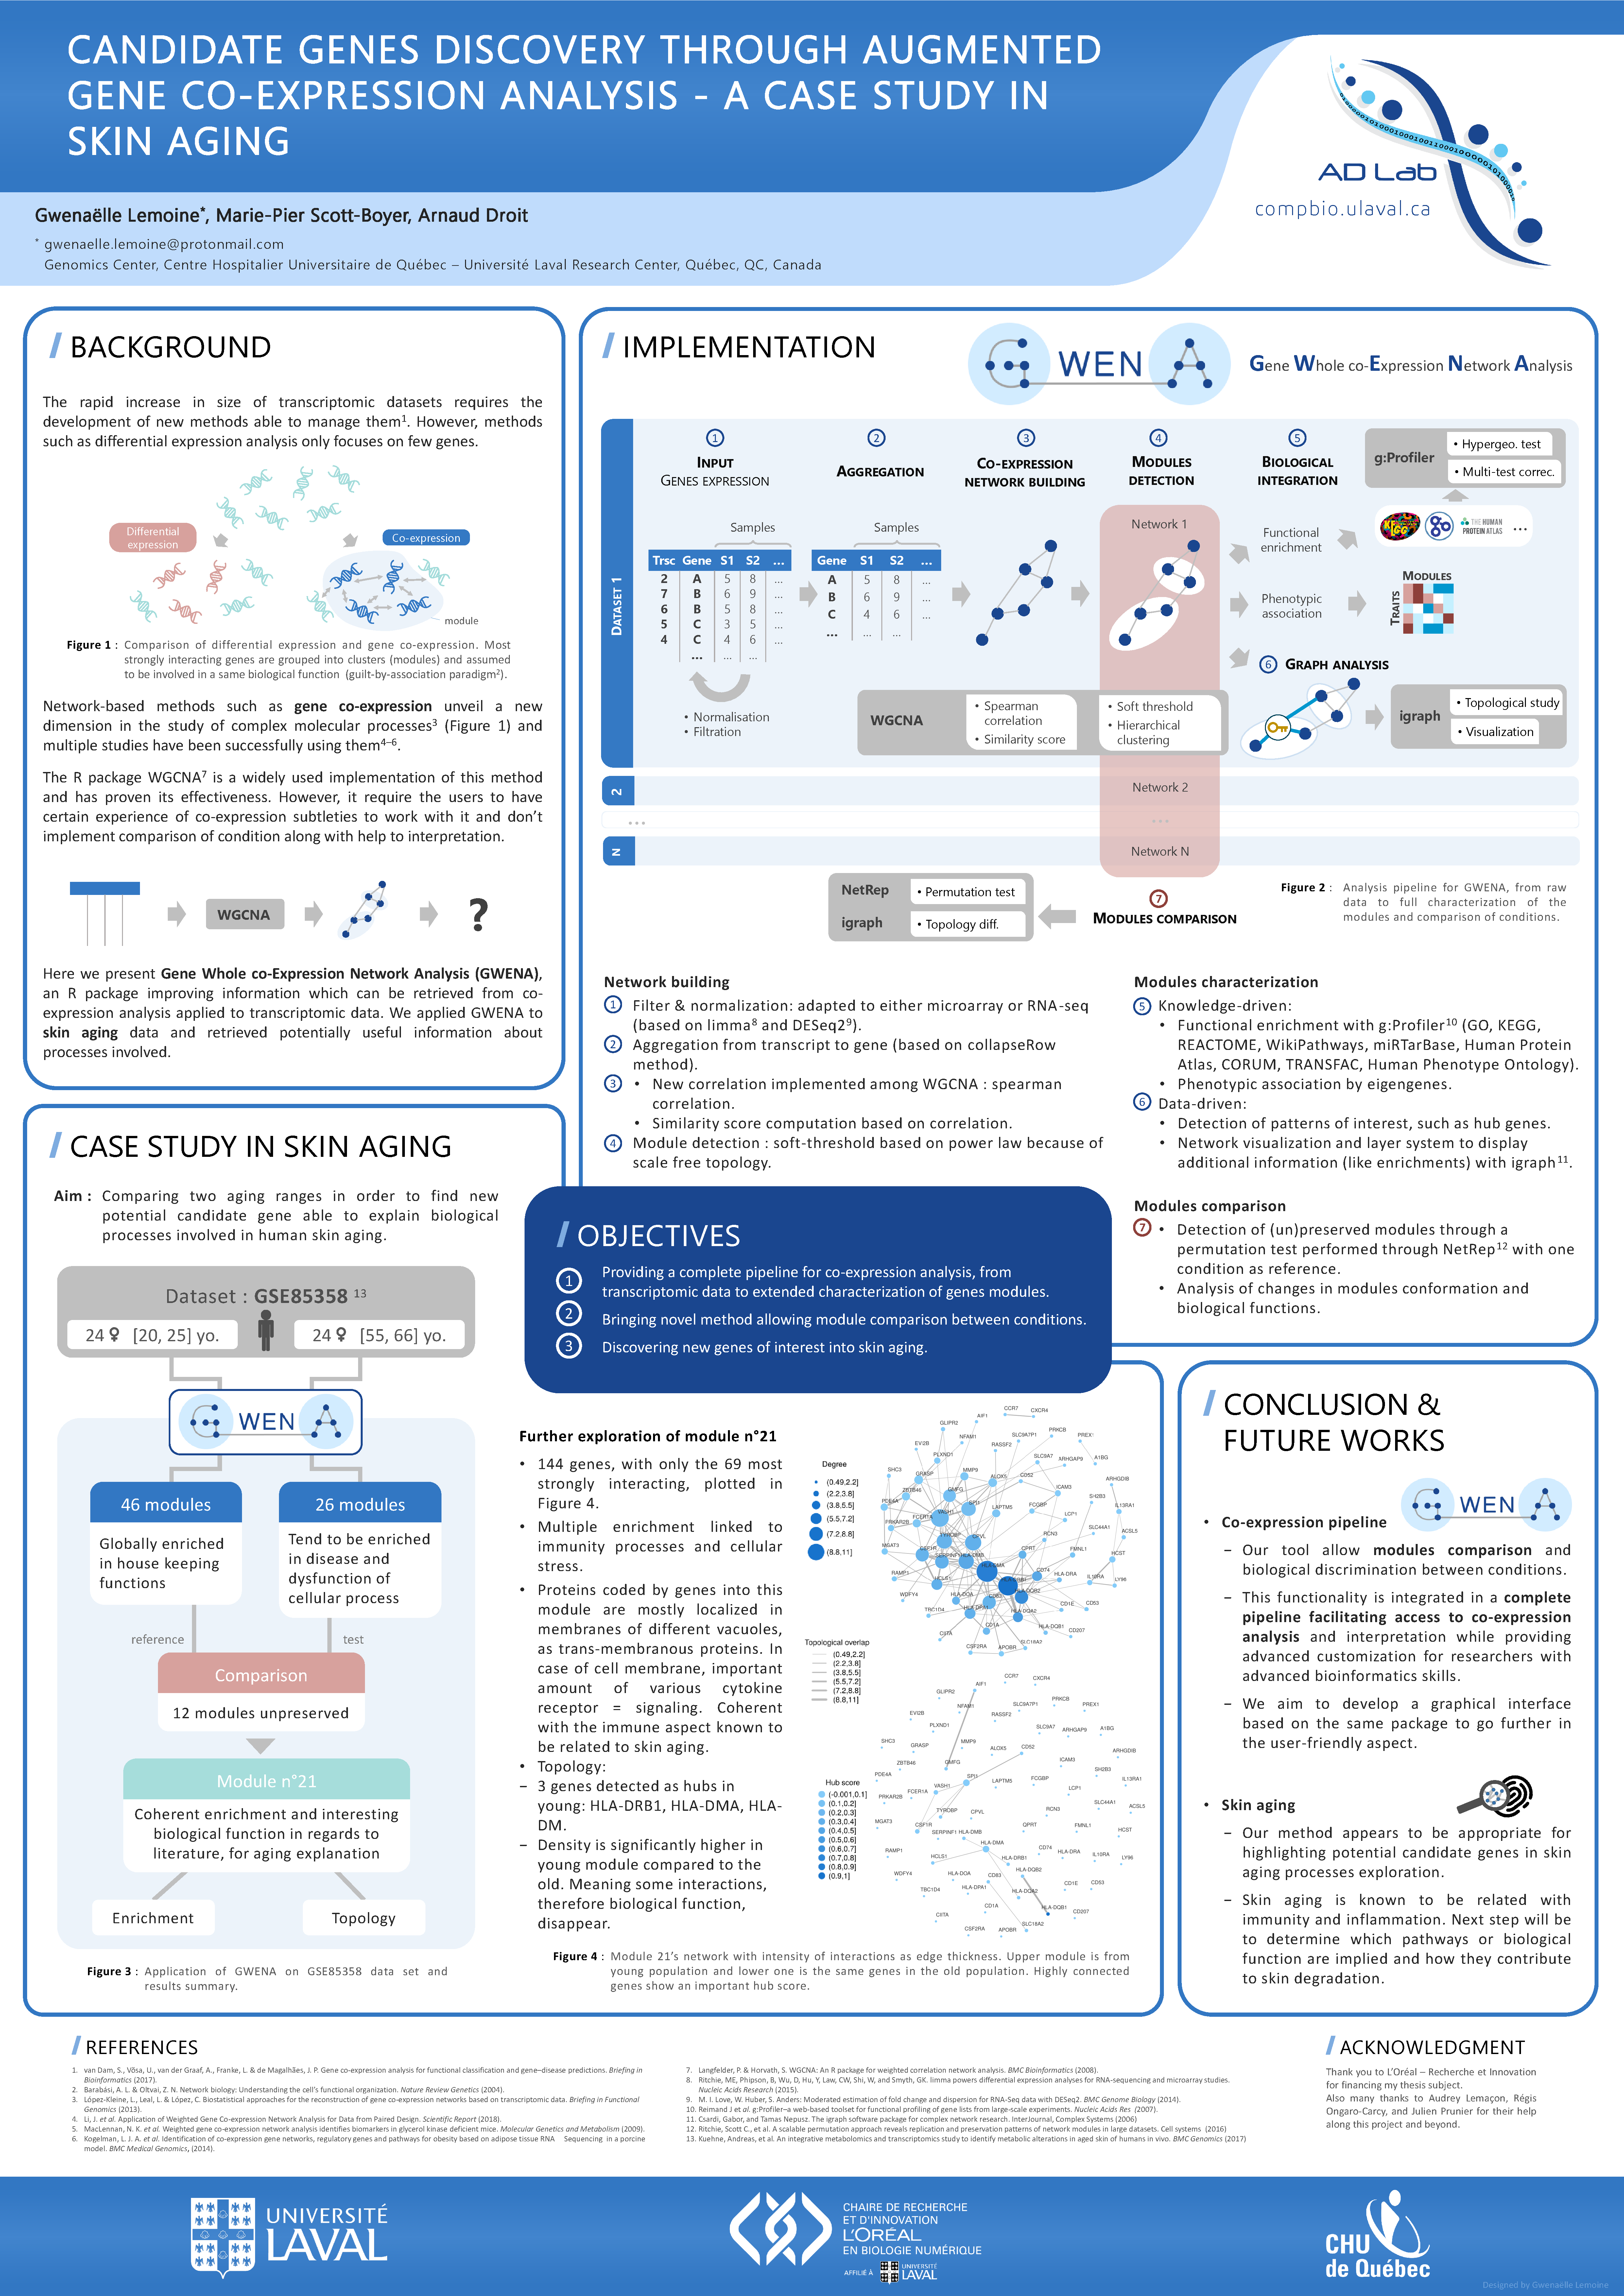
\includegraphics[width=\textwidth]{img/annexe_projets_annexe/20190700_ISCMECCB_ppt.pdf}
    \caption{Affiche présentée à la bi-conférence internationale ISMB/ECCB en 2019}
    \label{fig:annexe_poster_ismb_eccb}
\end{figure}

\begin{figure}
    \centering
    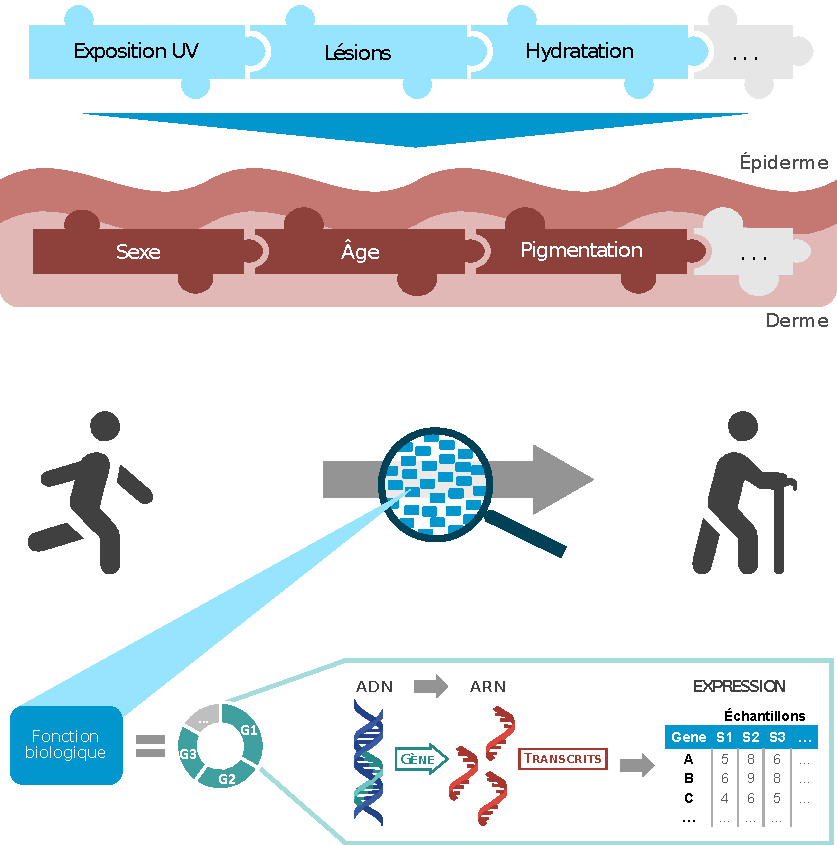
\includegraphics{img/annexe_projets_annexe/20190312_TeaAndLearn_ReuLabo_avancement.pdf}
    \caption[Illustration de la contribution des facteurs intrinsèques et extrinsèques au vieillissement de la peau et leur perception via l'expression des gènes]{Illustration de la contribution des facteurs intrinsèques et extrinsèques au vieillissement de la peau et leur perception via l'expression des gènes. Réalisé pour une présentation de séminaire étudiant au CHU de Québec-Université Laval.}
    \label{fig:annexe_schema_aging_skin_transcripto}
\end{figure}

\begin{figure}
    \centering
    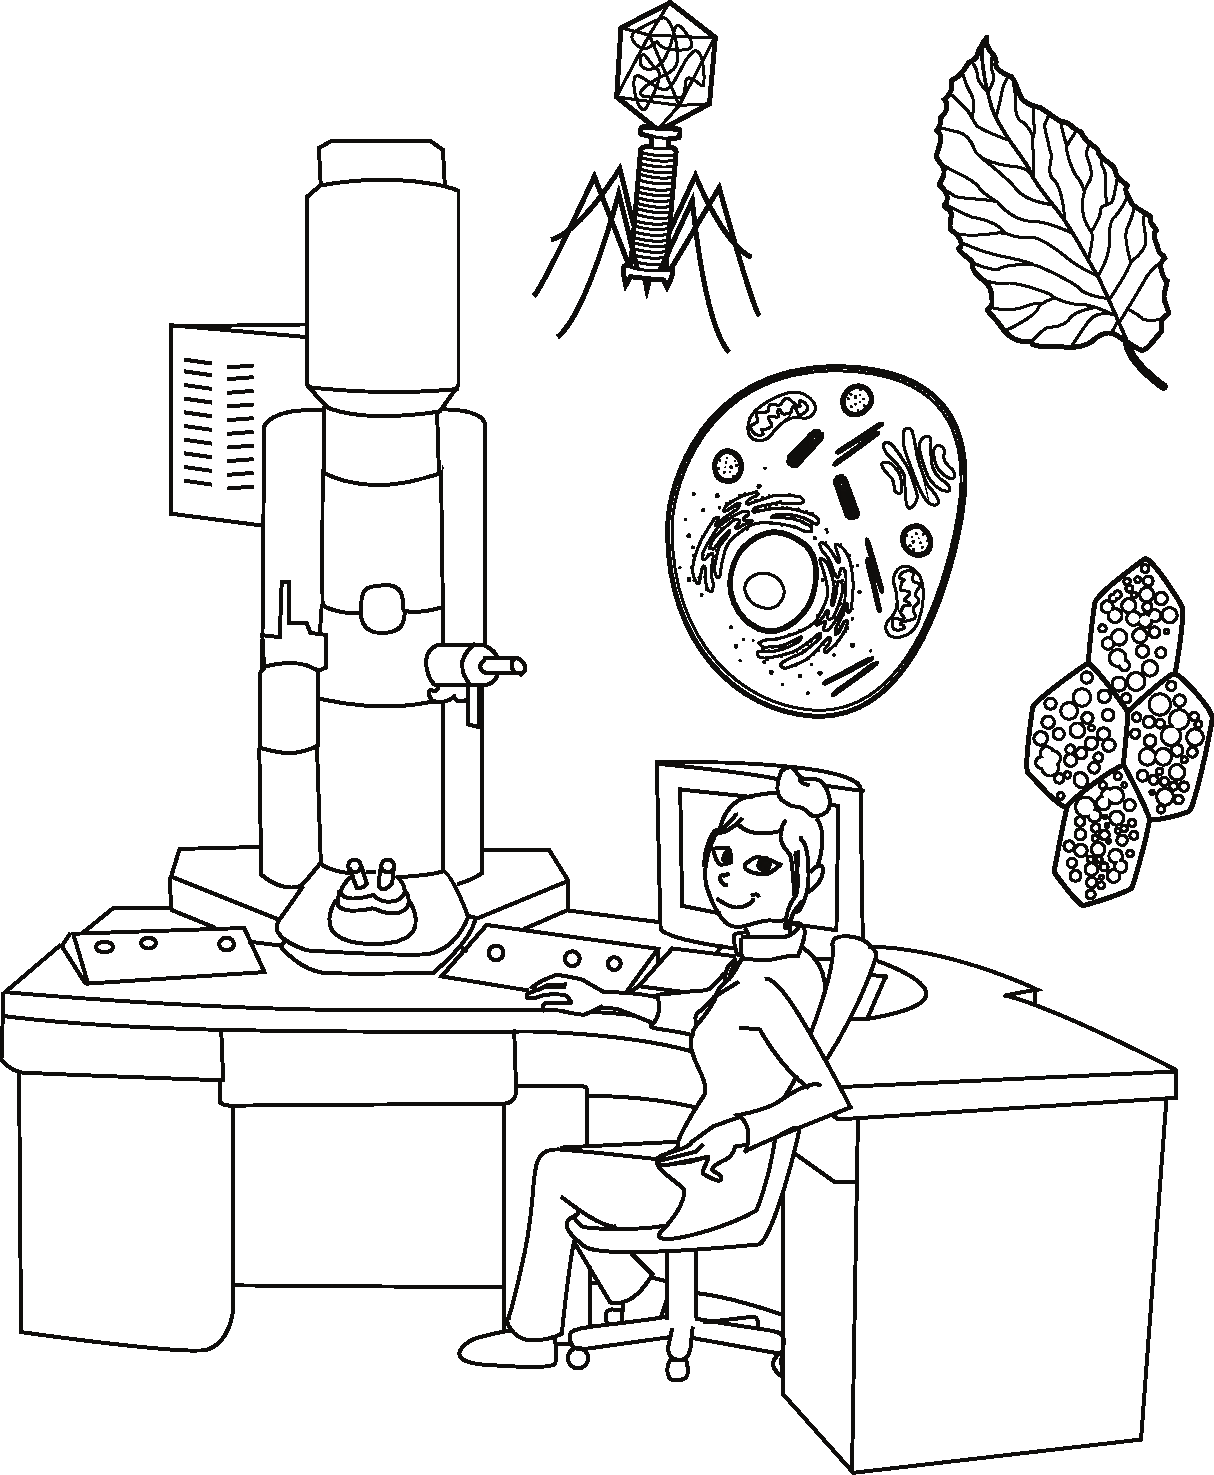
\includegraphics[width=0.8\textwidth]{img/annexe_projets_annexe/these_amandine.pdf}
    \caption[Ensemble d'illustrations réalisées pour la thèse d'Amandine Verguet en microscopie électronique en transmission appliquée à des échantillons biologiques]{Ensemble d'illustrations réalisées pour la thèse d'Amandine Verguet en microscopie électronique en transmission appliquée à des échantillons biologiques \cite{Verguet2019Dec}}
    \label{fig:annexe_these_amandine}
\end{figure}

\end{appendices}


% \chapter*{Glossaire}                                        % enlève la numérotation
\phantomsection\addcontentsline{toc}{chapter}{Glossaire}    % inclus le glossaire dans la table des matières

\printglossary[nonumberlist]
\glsaddall

%% MODELE
%\newglossaryentry{}
%{
%	name={},
%	description={}, 
%	plural={}
%}

\newglossaryentry{mecanisme}
{
	name={m\'{e}canisme},
	description={ensemble des acteurs cellulaires et moléculaires intervenant dans la réalisation d'une manifestation d'un phénomène \cite{Bechtel2013}}, 
	plural={m\'{e}canismes}
}

\newglossaryentry{fonction_biologique}
{
	name={Fonction biologique},
	description={terme ambigu pouvant désigner de nombreux concepts en biologie. Aussi dans cette thèse on s'appliquera à préciser au maximum son sens à l'aide du modèle de Pittsburg \cite{Marie2019}:
	\begin{description}
	    \item \textit{Implications évolutives} : l'influence de l'objet sur la dynamique de la population au cours de générations successives, telle qu'elle est rendue possible par ses implications physiologiques et leur interaction avec les pressions environnementales.
	    \item \textit{Implications physiologiques} : l'implication de l'objet dans les processus biologiques, telle qu'elle est rendue possible par un ensemble de capacités, d'interactions et de modèles d'expression, indépendamment des considérations transgénérationnelles.
	    \item \textit{Interactions} : les contacts physiques, directs ou indirects, entre l'objet étudié et les autres composants d'un système, y compris les contacts qui servent de médiateurs aux transformations chimiques.
	    \item \textit{Capacités} : les propriétés physiques intrinsèques de l'objet étudié ; la nécessité du comportement de l'objet compte tenu de son environnement (par exemple, les contraintes structurelles)
	    \item \textit{Expression} : la présence ou la quantité de l'objet étudié (objet ARN ou protéine), ou la présence ou la quantité de ses produits de transcription ou de traduction (objet ADN).
	    \item \textit{Vague} : On n'a pas trouvé de preuves suffisantes pour déduire une ou plusieurs significations de la fonction dans ce modèle, ni pour dériver une nouvelle signification.
	\end{description}
	}, 
	plural={Fonctions biologiques}
}


% \newglossaryentry{esptopo}
% {
% 	name={espace topologique},
% 	description={(mathématiques) ensemble muni d'une structure très générale (la topologie), qui permet de définir la notion de voisinage d'un point. Cette structure (la topologie) offre le langage pour définir les notions de continuité et de limite. Deux définitions équivalentes sont souvent données : la définition par les ouverts, et la définition par les voisinages d'un point
% 	\begin{description}
% 		\item [\emph{Par les ouverts}] : couple (E, T), où E est un ensemble et T une topologie sur E, à savoir un ensemble de parties de E — que l'on appelle les ouverts de (E, T);
% 		\item [\emph{Par les voisinages}] : Un espace topologique est un couple $(E,\mathcal {V})$, où $E$ est un ensemble et $\mathcal {V}$ une application de $E$ vers l'ensemble $P(P(E))$ obéissant aux cinq conditions ci-après, dans lesquelles les éléments de $\mathcal {V}(a)$, pour $a \in E$, sont appelés « voisinages de $a$ ». Pour tout point $a$ de $E$ :
% 		\begin{itemize}
% 			\item tout sur-ensemble d'un voisinage de $a$ est lui-même voisinage de $a$ ;
% 			\item l'intersection de deux voisinages de $a$ est elle-même un voisinage de $a$ ;
% 			\item $E$ est un voisinage de $a$ ;
% 			\item tout voisinage de $a$ contient $a$ ;
% 			\item pour tout voisinage $V$ de $a$, il existe un voisinage $W$ de $a$ tel que $V$ soit voisinage de chacun des points de $W$.
% 		\end{itemize}
% 	\end{description}},
% 	plural={espaces topologiques}
% }

% \newglossaryentry{partie}
% {
% 	name={partie},
% 	description={(mathématiques) Sous ensemble dont tous les éléments se trouvent dans un ensemble l'incluant}, 
% 	plural={parties}
% }

% \newglossaryentry{degree}
% {
% 	name={degr\'e},
% 	description={(mathématiques)(théorie des graphes) nombre de liens (arêtes ou arcs) reliant un sommet, avec les boucles comptées deux fois}, 
% 	plural={degr\'es},
% 	sort={degree}
% }

% \newglossaryentry{powerLaw}
% {
% 	name={loi de puissance},
% 	description={[\textit{power law}] (mathématiques) relation entre deux quantités x et y qui peut s'écrire de la façon suivante : \(y=ax^{k}\)}, 
% 	plural={lois de puissance}
% }

% \newglossaryentry{scaleFreeNet}
% {
% 	name={r\'eseau invariant d'échelle},
% 	description={[\textit{scale free network}] (mathématiques) réseau dont les degrés suivent une loi de puissance. C'est à dire un réseau où la proportion de nœuds de degré $k$ est proportionnelle à $k^{-\gamma}$ pour $k$ grand, où $\gamma$ est un paramètre (situé entre 2 et 3 pour la plupart des applications car en deçà ce n'est plus une loi de puissance, et au delà par nature cela réduirait ou augmenterait beaucoup trop l'espace de définition, ce qui devient dur à modéliser sur un plot)}, 
% 	plural={r\'eseaux invariants d'échelle},
% 	sort={reeseau invariant d'eechelle}
% }

% \newglossaryentry{topologie}
% {
% 	name={topologie},
% 	description={(mathématiques) Une topologie sur un ensemble $E$ est une famille $O \subset P(E)$ de parties de $E$ vérifiant 3 conditions : 
% 	\begin{itemize}
% 		\item $\varnothing$ et $E$ sont des éléments de $O$;
% 		\item Toute réunion d'éléments de $O$ est un élément de $O$;
% 		\item Toute intersection finie d'éléments de $O$ est un élément de $O$.
% 	\end{itemize}
% 	Les éléments de $O$ sont appelés les ouverts de la topologie. Le couple $(E, O)$ est appelé un espace topologique.\\\emph{Exemple} : L'ensemble $E=\{1,2,3\}$ peut être muni de 29 topologies
% 	\begin{itemize}
% 		\item $O_1 = \{\varnothing, E\}$
% 		\item $O_2 = \{\varnothing, \{1\}, E\}$
% 		\item $O_3 = \{\varnothing, \{1\}, \{1,2\}, E\}$
% 		\item $O_4 = \{\varnothing, \{1\}, \{1,2\}, \{1,3\}, E\}$
% 		\item $O_5 = \{\varnothing, \{2\}, \{1,2\}, \{2,3\}, E\}$
% 		\item $O_6 = \{\varnothing, \{1\}, \{2\}, \{1,2\}, \{1,3\}, E\}$
% 		\item \dots
% 	\end{itemize}},
% 	plural={topologies}
% }

% \newglossaryentry{ensemble}
% {
% 	name={ensemble},
% 	description={(mathématiques) collection d’objets (les éléments de l'ensemble) qui peuvent être compris comme un tout. Se note $E$}, 
% 	plural={ensembles}
% }

% \newglossaryentry{ensembleDesPart}
% {
% 	name={ensemble des parties},
% 	description={(mathématiques) Ensemble des sous-ensembles de cet ensemble. Se note $P(E)$.\\\emph{Exemple} : Soit $E$ un ensemble tel que $E=\{1,2,3\}$, alors $P(E)=\{\{a\},\{b\},\{c\},\{a,b\},\{a,c\},\{b,c\} ,\{a,b,c\},\{\varnothing\}\}$}, 
% 	plural={ensembles des parties}
% }

% \newglossaryentry{ouvert}
% {
% 	name={ouvert},
% 	description={(mathématiques)(topologie) aussi appelé ensemble ouvert ou une partie ouverte, un ouvert est un sous-ensemble d'un espace topologique qui ne contient aucun point de sa frontière\\\emph{Exemple} : Les points $(x, y)$ qui satisfont à l'équation $x^2 + y^2 = r^2$, soit un cercle, forment la frontière d'un espace topologique. Les points tels que $x^2 + y^2 < r^2$ forment un ensemble ouvert. L'union de cette frontière et de cet ensemble ouvert forme un ensemble fermé}, 
% 	plural={ouverts}
% }

% \newglossaryentry{recouvrement}
% {
% 	name={recouvrement},
% 	description={[\textit{overlap}] (mathématiques) Le recouvrement d'un ensemble $E$ est une famille $(X_i)_{i\in I}$ d'ensembles dont l'union contient $E$ (c'est à dire que tout élément de $E$ appartient au moins à l'un des $X_i$)},
% 	plural={recouvrements}
% }

% \newglossaryentry{QTL}
% {
% 	name={locus de caract\`eres quantitatifs},
% 	description={[\textit{quantitative trait locus}] (biologie) région plus ou moins grande d'ADN qui est étroitement associée à un caractère quantitatif, c'est-à-dire une région chromosomique où sont localisés un ou plusieurs gènes à l'origine du caractère en question}, 
% 	plural={loci de caract\`eres quantitatifs}
% }

% \newglossaryentry{autosome}
% {
% 	name={autosome},
% 	description={(biologie) chromosome non sexuel}, 
% 	plural={autosomes}
% }

% \newglossaryentry{gonosome}
% {
% 	name={gonosome},
% 	description={(biologie) chromosome sexuel}, 
% 	plural={gonosomes}
% }

% \newglossaryentry{ADNgenomiq}
% {
% 	name={ADN g\'enomique},
% 	description={(biologie) ADN se situant dans le nucléole, lui même se situant dans le noyau}, 
% 	plural={ADNs g\'enomiques}
% }

% \newglossaryentry{hubGene}
% {
% 	name={hub gene},
% 	description={(biostatistique) gène d'un module qui tend à avoir une très forte connectivité intra-modulaire. Il est généralement très fortement corrélé avec l'eigengene du même module}, 
% 	plural={hub genes}
% }

% \newglossaryentry{eigengene}
% {
% 	name={eigengene},
% 	description={(biostatistiques) L'eigengene d'un module de gènes est la première composante principale de ce module. Il peut être considéré comme le représentant des profils d'expression des gènes présents dans le module}, 
% 	plural={eigengene}
% }

% \newglossaryentry{geneSignif}
% {
% 	name={importance significative d'un g\`ene},
% 	description={[\textit{gene significance}] (bio-statistiques) valeur absolue de la corrélation entre un gène et un trait phénotypique }, 
% 	plural={importance significative de g\`enes}
% }

% \newglossaryentry{geneMember}
% {
% 	name={appartenance d'un g\`ene},
% 	description={[\textit{gene membership}] (biostatistiques) corrélation entre l'eigengene d'un module et le profil d'expression d'un gène}, 
% 	plural={appartenance de g\`enes}
% }





             % glossaire


\end{document}




